\documentclass[twoside]{book}

% Packages required by doxygen
\usepackage{calc}
\usepackage{doxygen}
\usepackage{graphicx}
\usepackage[utf8]{inputenc}
\usepackage{makeidx}
\usepackage{multicol}
\usepackage{multirow}
\usepackage{textcomp}
\usepackage[table]{xcolor}

% Font selection
\usepackage[T1]{fontenc}
\usepackage{mathptmx}
\usepackage[scaled=.90]{helvet}
\usepackage{courier}
\usepackage{amssymb}
\usepackage{sectsty}
\renewcommand{\familydefault}{\sfdefault}
\allsectionsfont{%
  \fontseries{bc}\selectfont%
  \color{darkgray}%
}
\renewcommand{\DoxyLabelFont}{%
  \fontseries{bc}\selectfont%
  \color{darkgray}%
}

% Page & text layout
\usepackage{geometry}
\geometry{%
  a4paper,%
  top=2.5cm,%
  bottom=2.5cm,%
  left=2.5cm,%
  right=2.5cm%
}
\tolerance=750
\hfuzz=15pt
\hbadness=750
\setlength{\emergencystretch}{15pt}
\setlength{\parindent}{0cm}
\setlength{\parskip}{0.2cm}
\makeatletter
\renewcommand{\paragraph}{%
  \@startsection{paragraph}{4}{0ex}{-1.0ex}{1.0ex}{%
    \normalfont\normalsize\bfseries\SS@parafont%
  }%
}
\renewcommand{\subparagraph}{%
  \@startsection{subparagraph}{5}{0ex}{-1.0ex}{1.0ex}{%
    \normalfont\normalsize\bfseries\SS@subparafont%
  }%
}
\makeatother

% Headers & footers
\usepackage{fancyhdr}
\pagestyle{fancyplain}
\fancyhead[LE]{\fancyplain{}{\bfseries\thepage}}
\fancyhead[CE]{\fancyplain{}{}}
\fancyhead[RE]{\fancyplain{}{\bfseries\leftmark}}
\fancyhead[LO]{\fancyplain{}{\bfseries\rightmark}}
\fancyhead[CO]{\fancyplain{}{}}
\fancyhead[RO]{\fancyplain{}{\bfseries\thepage}}
\fancyfoot[LE]{\fancyplain{}{}}
\fancyfoot[CE]{\fancyplain{}{}}
\fancyfoot[RE]{\fancyplain{}{\bfseries\scriptsize Generated on Wed Sep 18 2013 01\-:32\-:27 for King Test by Doxygen }}
\fancyfoot[LO]{\fancyplain{}{\bfseries\scriptsize Generated on Wed Sep 18 2013 01\-:32\-:27 for King Test by Doxygen }}
\fancyfoot[CO]{\fancyplain{}{}}
\fancyfoot[RO]{\fancyplain{}{}}
\renewcommand{\footrulewidth}{0.4pt}
\renewcommand{\chaptermark}[1]{%
  \markboth{#1}{}%
}
\renewcommand{\sectionmark}[1]{%
  \markright{\thesection\ #1}%
}

% Indices & bibliography
\usepackage{natbib}
\usepackage[titles]{tocloft}
\setcounter{tocdepth}{3}
\setcounter{secnumdepth}{5}
\makeindex

% Hyperlinks (required, but should be loaded last)
\usepackage{ifpdf}
\ifpdf
  \usepackage[pdftex,pagebackref=true]{hyperref}
\else
  \usepackage[ps2pdf,pagebackref=true]{hyperref}
\fi
\hypersetup{%
  colorlinks=true,%
  linkcolor=blue,%
  citecolor=blue,%
  unicode%
}

% Custom commands
\newcommand{\clearemptydoublepage}{%
  \newpage{\pagestyle{empty}\cleardoublepage}%
}


%===== C O N T E N T S =====

\begin{document}

% Titlepage & ToC
\hypersetup{pageanchor=false}
\pagenumbering{roman}
\begin{titlepage}
\vspace*{7cm}
\begin{center}%
{\Large King Test }\\
\vspace*{1cm}
{\large Generated by Doxygen 1.8.5}\\
\vspace*{0.5cm}
{\small Wed Sep 18 2013 01:32:27}\\
\end{center}
\end{titlepage}
\clearemptydoublepage
\tableofcontents
\clearemptydoublepage
\pagenumbering{arabic}
\hypersetup{pageanchor=true}

%--- Begin generated contents ---
\chapter{Hierarchical Index}
\section{Class Hierarchy}
This inheritance list is sorted roughly, but not completely, alphabetically\-:\begin{DoxyCompactList}
\item \contentsline{section}{tinyxml2\-:\-:Dyn\-Array$<$ T, I\-N\-I\-T $>$}{\pageref{classtinyxml2_1_1_dyn_array}}{}
\item \contentsline{section}{tinyxml2\-:\-:Dyn\-Array$<$ Block $\ast$, 10 $>$}{\pageref{classtinyxml2_1_1_dyn_array}}{}
\item \contentsline{section}{tinyxml2\-:\-:Dyn\-Array$<$ char, 20 $>$}{\pageref{classtinyxml2_1_1_dyn_array}}{}
\item \contentsline{section}{tinyxml2\-:\-:Dyn\-Array$<$ const char $\ast$, 10 $>$}{\pageref{classtinyxml2_1_1_dyn_array}}{}
\item \contentsline{section}{tinyxml2\-:\-:Entity}{\pageref{structtinyxml2_1_1_entity}}{}
\item \contentsline{section}{Game}{\pageref{class_game}}{}
\item \contentsline{section}{Game\-Board}{\pageref{class_game_board}}{}
\item \contentsline{section}{Game\-Logic}{\pageref{class_game_logic}}{}
\item \contentsline{section}{Game\-Piece}{\pageref{class_game_piece}}{}
\item \contentsline{section}{Game\-Renderer}{\pageref{class_game_renderer}}{}
\item \contentsline{section}{Game\-Timer}{\pageref{class_game_timer}}{}
\item \contentsline{section}{Interpolator}{\pageref{class_interpolator}}{}
\item \contentsline{section}{Linear\-Allocator}{\pageref{class_linear_allocator}}{}
\item \contentsline{section}{Game\-Board\-:\-:Match\-Result}{\pageref{struct_game_board_1_1_match_result}}{}
\item \contentsline{section}{tinyxml2\-:\-:Mem\-Pool}{\pageref{classtinyxml2_1_1_mem_pool}}{}
\begin{DoxyCompactList}
\item \contentsline{section}{tinyxml2\-:\-:Mem\-Pool\-T$<$ sizeof(tinyxml2\-:\-:X\-M\-L\-Attribute) $>$}{\pageref{classtinyxml2_1_1_mem_pool_t}}{}
\item \contentsline{section}{tinyxml2\-:\-:Mem\-Pool\-T$<$ sizeof(tinyxml2\-:\-:X\-M\-L\-Comment) $>$}{\pageref{classtinyxml2_1_1_mem_pool_t}}{}
\item \contentsline{section}{tinyxml2\-:\-:Mem\-Pool\-T$<$ sizeof(tinyxml2\-:\-:X\-M\-L\-Element) $>$}{\pageref{classtinyxml2_1_1_mem_pool_t}}{}
\item \contentsline{section}{tinyxml2\-:\-:Mem\-Pool\-T$<$ sizeof(tinyxml2\-:\-:X\-M\-L\-Text) $>$}{\pageref{classtinyxml2_1_1_mem_pool_t}}{}
\item \contentsline{section}{tinyxml2\-:\-:Mem\-Pool\-T$<$ S\-I\-Z\-E $>$}{\pageref{classtinyxml2_1_1_mem_pool_t}}{}
\end{DoxyCompactList}
\item \contentsline{section}{Region}{\pageref{struct_region}}{}
\item \contentsline{section}{Sprite}{\pageref{struct_sprite}}{}
\item \contentsline{section}{tinyxml2\-:\-:Str\-Pair}{\pageref{classtinyxml2_1_1_str_pair}}{}
\item \contentsline{section}{Texture\-Atlas}{\pageref{class_texture_atlas}}{}
\item \contentsline{section}{Texture\-Atlas\-Data}{\pageref{struct_texture_atlas_data}}{}
\item \contentsline{section}{T\-Link$<$ T $>$}{\pageref{class_t_link}}{}
\item \contentsline{section}{T\-List$<$ T $>$}{\pageref{class_t_list}}{}
\begin{DoxyCompactList}
\item \contentsline{section}{T\-List\-Declare$<$ T, offset $>$}{\pageref{class_t_list_declare}}{}
\end{DoxyCompactList}
\item \contentsline{section}{king\-:\-:renderer\-:\-:Vert}{\pageref{structking_1_1renderer_1_1_vert}}{}
\item \contentsline{section}{tinyxml2\-:\-:X\-M\-L\-Attribute}{\pageref{classtinyxml2_1_1_x_m_l_attribute}}{}
\item \contentsline{section}{tinyxml2\-:\-:X\-M\-L\-Const\-Handle}{\pageref{classtinyxml2_1_1_x_m_l_const_handle}}{}
\item \contentsline{section}{tinyxml2\-:\-:X\-M\-L\-Handle}{\pageref{classtinyxml2_1_1_x_m_l_handle}}{}
\item \contentsline{section}{tinyxml2\-:\-:X\-M\-L\-Node}{\pageref{classtinyxml2_1_1_x_m_l_node}}{}
\begin{DoxyCompactList}
\item \contentsline{section}{tinyxml2\-:\-:X\-M\-L\-Comment}{\pageref{classtinyxml2_1_1_x_m_l_comment}}{}
\item \contentsline{section}{tinyxml2\-:\-:X\-M\-L\-Declaration}{\pageref{classtinyxml2_1_1_x_m_l_declaration}}{}
\item \contentsline{section}{tinyxml2\-:\-:X\-M\-L\-Document}{\pageref{classtinyxml2_1_1_x_m_l_document}}{}
\item \contentsline{section}{tinyxml2\-:\-:X\-M\-L\-Element}{\pageref{classtinyxml2_1_1_x_m_l_element}}{}
\item \contentsline{section}{tinyxml2\-:\-:X\-M\-L\-Text}{\pageref{classtinyxml2_1_1_x_m_l_text}}{}
\item \contentsline{section}{tinyxml2\-:\-:X\-M\-L\-Unknown}{\pageref{classtinyxml2_1_1_x_m_l_unknown}}{}
\end{DoxyCompactList}
\item \contentsline{section}{tinyxml2\-:\-:X\-M\-L\-Util}{\pageref{classtinyxml2_1_1_x_m_l_util}}{}
\item \contentsline{section}{tinyxml2\-:\-:X\-M\-L\-Visitor}{\pageref{classtinyxml2_1_1_x_m_l_visitor}}{}
\begin{DoxyCompactList}
\item \contentsline{section}{tinyxml2\-:\-:X\-M\-L\-Printer}{\pageref{classtinyxml2_1_1_x_m_l_printer}}{}
\end{DoxyCompactList}
\end{DoxyCompactList}

\chapter{Class Index}
\section{Class List}
Here are the classes, structs, unions and interfaces with brief descriptions\-:\begin{DoxyCompactList}
\item\contentsline{section}{\hyperlink{classtinyxml2_1_1_dyn_array}{tinyxml2\-::\-Dyn\-Array$<$ T, I\-N\-I\-T $>$} }{\pageref{classtinyxml2_1_1_dyn_array}}{}
\item\contentsline{section}{\hyperlink{structtinyxml2_1_1_entity}{tinyxml2\-::\-Entity} }{\pageref{structtinyxml2_1_1_entity}}{}
\item\contentsline{section}{\hyperlink{class_game}{Game} \\*\hyperlink{class_game}{Game} is the main entry point of the game. It contains the main loop and handles gameplay and rendering }{\pageref{class_game}}{}
\item\contentsline{section}{\hyperlink{class_game_board}{Game\-Board} \\*This class handle the game board from a logical point of view }{\pageref{class_game_board}}{}
\item\contentsline{section}{\hyperlink{class_game_logic}{Game\-Logic} }{\pageref{class_game_logic}}{}
\item\contentsline{section}{\hyperlink{class_game_piece}{Game\-Piece} }{\pageref{class_game_piece}}{}
\item\contentsline{section}{\hyperlink{class_game_renderer}{Game\-Renderer} }{\pageref{class_game_renderer}}{}
\item\contentsline{section}{\hyperlink{class_game_timer}{Game\-Timer} \\*This class handles timed event in game trough callbacks }{\pageref{class_game_timer}}{}
\item\contentsline{section}{\hyperlink{class_interpolator}{Interpolator} \\*This class handles interpolation of a given float reference }{\pageref{class_interpolator}}{}
\item\contentsline{section}{\hyperlink{class_linear_allocator}{Linear\-Allocator} \\*Lienar allocator allocate sequential objects, object cannot be destoied arbitrairly }{\pageref{class_linear_allocator}}{}
\item\contentsline{section}{\hyperlink{struct_game_board_1_1_match_result}{Game\-Board\-::\-Match\-Result} \\*Query result data structure }{\pageref{struct_game_board_1_1_match_result}}{}
\item\contentsline{section}{\hyperlink{classtinyxml2_1_1_mem_pool}{tinyxml2\-::\-Mem\-Pool} }{\pageref{classtinyxml2_1_1_mem_pool}}{}
\item\contentsline{section}{\hyperlink{classtinyxml2_1_1_mem_pool_t}{tinyxml2\-::\-Mem\-Pool\-T$<$ S\-I\-Z\-E $>$} }{\pageref{classtinyxml2_1_1_mem_pool_t}}{}
\item\contentsline{section}{\hyperlink{struct_region}{Region} \\*\hyperlink{struct_region}{Region} of the texture atlas }{\pageref{struct_region}}{}
\item\contentsline{section}{\hyperlink{struct_sprite}{Sprite} \\*data for a sprite }{\pageref{struct_sprite}}{}
\item\contentsline{section}{\hyperlink{classtinyxml2_1_1_str_pair}{tinyxml2\-::\-Str\-Pair} }{\pageref{classtinyxml2_1_1_str_pair}}{}
\item\contentsline{section}{\hyperlink{class_texture_atlas}{Texture\-Atlas} \\*\hyperlink{class_texture_atlas}{Texture\-Atlas} handle the textures and their instances , keeping track of them and upload them to the G\-P\-U }{\pageref{class_texture_atlas}}{}
\item\contentsline{section}{\hyperlink{struct_texture_atlas_data}{Texture\-Atlas\-Data} \\*Brief pimpl \-: define internal state here to make the interface more clear and avoid depencies }{\pageref{struct_texture_atlas_data}}{}
\item\contentsline{section}{\hyperlink{class_t_link}{T\-Link$<$ T $>$} }{\pageref{class_t_link}}{}
\item\contentsline{section}{\hyperlink{class_t_list}{T\-List$<$ T $>$} }{\pageref{class_t_list}}{}
\item\contentsline{section}{\hyperlink{class_t_list_declare}{T\-List\-Declare$<$ T, offset $>$} }{\pageref{class_t_list_declare}}{}
\item\contentsline{section}{\hyperlink{structking_1_1renderer_1_1_vert}{king\-::renderer\-::\-Vert} }{\pageref{structking_1_1renderer_1_1_vert}}{}
\item\contentsline{section}{\hyperlink{classtinyxml2_1_1_x_m_l_attribute}{tinyxml2\-::\-X\-M\-L\-Attribute} }{\pageref{classtinyxml2_1_1_x_m_l_attribute}}{}
\item\contentsline{section}{\hyperlink{classtinyxml2_1_1_x_m_l_comment}{tinyxml2\-::\-X\-M\-L\-Comment} }{\pageref{classtinyxml2_1_1_x_m_l_comment}}{}
\item\contentsline{section}{\hyperlink{classtinyxml2_1_1_x_m_l_const_handle}{tinyxml2\-::\-X\-M\-L\-Const\-Handle} }{\pageref{classtinyxml2_1_1_x_m_l_const_handle}}{}
\item\contentsline{section}{\hyperlink{classtinyxml2_1_1_x_m_l_declaration}{tinyxml2\-::\-X\-M\-L\-Declaration} }{\pageref{classtinyxml2_1_1_x_m_l_declaration}}{}
\item\contentsline{section}{\hyperlink{classtinyxml2_1_1_x_m_l_document}{tinyxml2\-::\-X\-M\-L\-Document} }{\pageref{classtinyxml2_1_1_x_m_l_document}}{}
\item\contentsline{section}{\hyperlink{classtinyxml2_1_1_x_m_l_element}{tinyxml2\-::\-X\-M\-L\-Element} }{\pageref{classtinyxml2_1_1_x_m_l_element}}{}
\item\contentsline{section}{\hyperlink{classtinyxml2_1_1_x_m_l_handle}{tinyxml2\-::\-X\-M\-L\-Handle} }{\pageref{classtinyxml2_1_1_x_m_l_handle}}{}
\item\contentsline{section}{\hyperlink{classtinyxml2_1_1_x_m_l_node}{tinyxml2\-::\-X\-M\-L\-Node} }{\pageref{classtinyxml2_1_1_x_m_l_node}}{}
\item\contentsline{section}{\hyperlink{classtinyxml2_1_1_x_m_l_printer}{tinyxml2\-::\-X\-M\-L\-Printer} }{\pageref{classtinyxml2_1_1_x_m_l_printer}}{}
\item\contentsline{section}{\hyperlink{classtinyxml2_1_1_x_m_l_text}{tinyxml2\-::\-X\-M\-L\-Text} }{\pageref{classtinyxml2_1_1_x_m_l_text}}{}
\item\contentsline{section}{\hyperlink{classtinyxml2_1_1_x_m_l_unknown}{tinyxml2\-::\-X\-M\-L\-Unknown} }{\pageref{classtinyxml2_1_1_x_m_l_unknown}}{}
\item\contentsline{section}{\hyperlink{classtinyxml2_1_1_x_m_l_util}{tinyxml2\-::\-X\-M\-L\-Util} }{\pageref{classtinyxml2_1_1_x_m_l_util}}{}
\item\contentsline{section}{\hyperlink{classtinyxml2_1_1_x_m_l_visitor}{tinyxml2\-::\-X\-M\-L\-Visitor} }{\pageref{classtinyxml2_1_1_x_m_l_visitor}}{}
\end{DoxyCompactList}

\chapter{Class Documentation}
\hypertarget{classtinyxml2_1_1_dyn_array}{\section{tinyxml2\-:\-:Dyn\-Array$<$ T, I\-N\-I\-T $>$ Class Template Reference}
\label{classtinyxml2_1_1_dyn_array}\index{tinyxml2\-::\-Dyn\-Array$<$ T, I\-N\-I\-T $>$@{tinyxml2\-::\-Dyn\-Array$<$ T, I\-N\-I\-T $>$}}
}
\subsection*{Public Member Functions}
\begin{DoxyCompactItemize}
\item 
\hypertarget{classtinyxml2_1_1_dyn_array_a498de53808ba0151fef54ea10bf51050}{void {\bfseries Push} (T t)}\label{classtinyxml2_1_1_dyn_array_a498de53808ba0151fef54ea10bf51050}

\item 
\hypertarget{classtinyxml2_1_1_dyn_array_aa3c360d40addc3b05121da9f60a01b4d}{T $\ast$ {\bfseries Push\-Arr} (int count)}\label{classtinyxml2_1_1_dyn_array_aa3c360d40addc3b05121da9f60a01b4d}

\item 
\hypertarget{classtinyxml2_1_1_dyn_array_a2281e3342bc235bf391a67e362c75866}{T {\bfseries Pop} ()}\label{classtinyxml2_1_1_dyn_array_a2281e3342bc235bf391a67e362c75866}

\item 
\hypertarget{classtinyxml2_1_1_dyn_array_ab45c0836d8c0260a5b9eda7da80de71c}{void {\bfseries Pop\-Arr} (int count)}\label{classtinyxml2_1_1_dyn_array_ab45c0836d8c0260a5b9eda7da80de71c}

\item 
\hypertarget{classtinyxml2_1_1_dyn_array_a080dc4dc68713964bb17745d4c833158}{bool {\bfseries Empty} () const }\label{classtinyxml2_1_1_dyn_array_a080dc4dc68713964bb17745d4c833158}

\item 
\hypertarget{classtinyxml2_1_1_dyn_array_a775a6ab4d41f0eb15bdd863d408dd58f}{T \& {\bfseries operator\mbox{[}$\,$\mbox{]}} (int i)}\label{classtinyxml2_1_1_dyn_array_a775a6ab4d41f0eb15bdd863d408dd58f}

\item 
\hypertarget{classtinyxml2_1_1_dyn_array_a1f4874c2608cbd68be1627fca9efd820}{const T \& {\bfseries operator\mbox{[}$\,$\mbox{]}} (int i) const }\label{classtinyxml2_1_1_dyn_array_a1f4874c2608cbd68be1627fca9efd820}

\item 
\hypertarget{classtinyxml2_1_1_dyn_array_a1299b257b62ea6b4983c488867f219b0}{int {\bfseries Size} () const }\label{classtinyxml2_1_1_dyn_array_a1299b257b62ea6b4983c488867f219b0}

\item 
\hypertarget{classtinyxml2_1_1_dyn_array_a8edbe90ed53b2e46b1b5cf53b261e4e7}{int {\bfseries Capacity} () const }\label{classtinyxml2_1_1_dyn_array_a8edbe90ed53b2e46b1b5cf53b261e4e7}

\item 
\hypertarget{classtinyxml2_1_1_dyn_array_a1f39330daeb97d3d1dc3fc12dcf7ac67}{const T $\ast$ {\bfseries Mem} () const }\label{classtinyxml2_1_1_dyn_array_a1f39330daeb97d3d1dc3fc12dcf7ac67}

\item 
\hypertarget{classtinyxml2_1_1_dyn_array_a0e0d60b399d54fad5b33d5008bc59c8e}{T $\ast$ {\bfseries Mem} ()}\label{classtinyxml2_1_1_dyn_array_a0e0d60b399d54fad5b33d5008bc59c8e}

\end{DoxyCompactItemize}


The documentation for this class was generated from the following file\-:\begin{DoxyCompactItemize}
\item 
tinyxml2.\-h\end{DoxyCompactItemize}

\hypertarget{structtinyxml2_1_1_entity}{\section{tinyxml2\-:\-:Entity Struct Reference}
\label{structtinyxml2_1_1_entity}\index{tinyxml2\-::\-Entity@{tinyxml2\-::\-Entity}}
}
\subsection*{Public Attributes}
\begin{DoxyCompactItemize}
\item 
\hypertarget{structtinyxml2_1_1_entity_ab330f5d665d29bfc811ecfa76315894b}{const char $\ast$ {\bfseries pattern}}\label{structtinyxml2_1_1_entity_ab330f5d665d29bfc811ecfa76315894b}

\item 
\hypertarget{structtinyxml2_1_1_entity_a25e2b57cb59cb4fa68f283d7cb570f21}{int {\bfseries length}}\label{structtinyxml2_1_1_entity_a25e2b57cb59cb4fa68f283d7cb570f21}

\item 
\hypertarget{structtinyxml2_1_1_entity_a7334e81e33b4615655a403711b24f3ed}{char {\bfseries value}}\label{structtinyxml2_1_1_entity_a7334e81e33b4615655a403711b24f3ed}

\end{DoxyCompactItemize}


The documentation for this struct was generated from the following file\-:\begin{DoxyCompactItemize}
\item 
tinyxml2.\-cpp\end{DoxyCompactItemize}

\hypertarget{class_game}{\section{Game Class Reference}
\label{class_game}\index{Game@{Game}}
}


\hyperlink{class_game}{Game} is the main entry point of the game. It contains the main loop and handles gameplay and rendering.  




{\ttfamily \#include $<$Game.\-h$>$}

\subsection*{Public Member Functions}
\begin{DoxyCompactItemize}
\item 
\hypertarget{class_game_ad59df6562a58a614fda24622d3715b65}{\hyperlink{class_game_ad59df6562a58a614fda24622d3715b65}{Game} ()}\label{class_game_ad59df6562a58a614fda24622d3715b65}

\begin{DoxyCompactList}\small\item\em default constructor \end{DoxyCompactList}\item 
\hypertarget{class_game_ae3d112ca6e0e55150d2fdbc704474530}{\hyperlink{class_game_ae3d112ca6e0e55150d2fdbc704474530}{$\sim$\-Game} ()}\label{class_game_ae3d112ca6e0e55150d2fdbc704474530}

\begin{DoxyCompactList}\small\item\em deconstructor \end{DoxyCompactList}\item 
\hypertarget{class_game_a555a9e4719fd49971765a2ab8b090b5c}{void \hyperlink{class_game_a555a9e4719fd49971765a2ab8b090b5c}{Init} ()}\label{class_game_a555a9e4719fd49971765a2ab8b090b5c}

\begin{DoxyCompactList}\small\item\em initialize the app \end{DoxyCompactList}\item 
\hypertarget{class_game_a96341ca5b54d90adc3ecb3bf0bcd2312}{void \hyperlink{class_game_a96341ca5b54d90adc3ecb3bf0bcd2312}{Run} ()}\label{class_game_a96341ca5b54d90adc3ecb3bf0bcd2312}

\begin{DoxyCompactList}\small\item\em the main loop \end{DoxyCompactList}\item 
\hypertarget{class_game_ad3b88fb61f44dbaaf88881cd77590958}{void \hyperlink{class_game_ad3b88fb61f44dbaaf88881cd77590958}{Shutdown} ()}\label{class_game_ad3b88fb61f44dbaaf88881cd77590958}

\begin{DoxyCompactList}\small\item\em tenrminate the app \end{DoxyCompactList}\end{DoxyCompactItemize}
\subsection*{Static Public Member Functions}
\begin{DoxyCompactItemize}
\item 
\hypertarget{class_game_a8a449b33a6bc286c427366a2657e1764}{static void \hyperlink{class_game_a8a449b33a6bc286c427366a2657e1764}{Update\-Step} (void $\ast$p\-Data)}\label{class_game_a8a449b33a6bc286c427366a2657e1764}

\begin{DoxyCompactList}\small\item\em callback called by the timer \end{DoxyCompactList}\end{DoxyCompactItemize}


\subsection{Detailed Description}
\hyperlink{class_game}{Game} is the main entry point of the game. It contains the main loop and handles gameplay and rendering. 

The documentation for this class was generated from the following files\-:\begin{DoxyCompactItemize}
\item 
Game.\-h\item 
Game.\-cpp\end{DoxyCompactItemize}

\hypertarget{class_game_board}{\section{Game\-Board Class Reference}
\label{class_game_board}\index{Game\-Board@{Game\-Board}}
}


this class handle the game board from a logical point of view  




{\ttfamily \#include $<$Game\-Board.\-h$>$}

\subsection*{Classes}
\begin{DoxyCompactItemize}
\item 
struct \hyperlink{struct_game_board_1_1_match_result}{Match\-Result}
\begin{DoxyCompactList}\small\item\em query result data structure \end{DoxyCompactList}\end{DoxyCompactItemize}
\subsection*{Public Types}
\begin{DoxyCompactItemize}
\item 
enum {\bfseries Direction} \{ {\bfseries R\-O\-W}, 
{\bfseries C\-O\-L}
 \}
\end{DoxyCompactItemize}
\subsection*{Public Member Functions}
\begin{DoxyCompactItemize}
\item 
\hypertarget{class_game_board_afed551e9c127df283a47e8124b1318a4}{\hyperlink{class_game_board_afed551e9c127df283a47e8124b1318a4}{Game\-Board} (unsigned int num\-Row, unsigned int num\-Col)}\label{class_game_board_afed551e9c127df283a47e8124b1318a4}

\begin{DoxyCompactList}\small\item\em create a board with the give size \end{DoxyCompactList}\item 
\hypertarget{class_game_board_a48e19b4953c87cc5eea1f9152d09499e}{\hyperlink{class_game_board_a48e19b4953c87cc5eea1f9152d09499e}{$\sim$\-Game\-Board} ()}\label{class_game_board_a48e19b4953c87cc5eea1f9152d09499e}

\begin{DoxyCompactList}\small\item\em destructor \end{DoxyCompactList}\item 
\hypertarget{class_game_board_aba09f382ac8efd967505bbcbe93ba8fc}{void \hyperlink{class_game_board_aba09f382ac8efd967505bbcbe93ba8fc}{Set\-Piece} (unsigned int x, unsigned int y, const \hyperlink{class_game_piece}{Game\-Piece} \&piece)}\label{class_game_board_aba09f382ac8efd967505bbcbe93ba8fc}

\begin{DoxyCompactList}\small\item\em set piece in the given position \end{DoxyCompactList}\item 
\hypertarget{class_game_board_a8ac26b97976d4fc0b80f74486eab45a1}{bool \hyperlink{class_game_board_a8ac26b97976d4fc0b80f74486eab45a1}{Swap\-Piece} (unsigned int x1, unsigned int y1, unsigned int x2, unsigned int y2)}\label{class_game_board_a8ac26b97976d4fc0b80f74486eab45a1}

\begin{DoxyCompactList}\small\item\em Swap the piece with a neighbor. \end{DoxyCompactList}\item 
\hypertarget{class_game_board_abc9f68a6a81a3ec70d07224e9309b67f}{void \hyperlink{class_game_board_abc9f68a6a81a3ec70d07224e9309b67f}{Set\-Region\-As\-Valid} (unsigned int x1, unsigned int y1, unsigned int x2, unsigned int y2)}\label{class_game_board_abc9f68a6a81a3ec70d07224e9309b67f}

\begin{DoxyCompactList}\small\item\em set the board rectangle as valid \end{DoxyCompactList}\item 
\hypertarget{class_game_board_a543bd5dbfa8b27bac058dd1aa8f4b40f}{void \hyperlink{class_game_board_a543bd5dbfa8b27bac058dd1aa8f4b40f}{Fill\-Valid\-Region\-With\-Colors} ()}\label{class_game_board_a543bd5dbfa8b27bac058dd1aa8f4b40f}

\begin{DoxyCompactList}\small\item\em fill regions with random colors \end{DoxyCompactList}\item 
\hypertarget{class_game_board_a345d5c2d3492cc61a9e67b8e85c4be9d}{void \hyperlink{class_game_board_a345d5c2d3492cc61a9e67b8e85c4be9d}{Get\-Grid\-Size} (int \&x, int \&y) const }\label{class_game_board_a345d5c2d3492cc61a9e67b8e85c4be9d}

\begin{DoxyCompactList}\small\item\em get the grid size \end{DoxyCompactList}\item 
\hypertarget{class_game_board_ae28369d503321f0f2cd444a87aa661a3}{const \hyperlink{class_game_piece}{Game\-Piece} \& \hyperlink{class_game_board_ae28369d503321f0f2cd444a87aa661a3}{Get\-Piece} (unsigned int x, unsigned int y) const }\label{class_game_board_ae28369d503321f0f2cd444a87aa661a3}

\begin{DoxyCompactList}\small\item\em get the piece \end{DoxyCompactList}\item 
\hypertarget{class_game_board_a14316a2356cc7ed2e0c7b89d250591b2}{\hyperlink{class_game_piece}{Game\-Piece} \& \hyperlink{class_game_board_a14316a2356cc7ed2e0c7b89d250591b2}{Get\-Piece} (unsigned int x, unsigned int y)}\label{class_game_board_a14316a2356cc7ed2e0c7b89d250591b2}

\begin{DoxyCompactList}\small\item\em non const get piece \end{DoxyCompactList}\item 
\hypertarget{class_game_board_a5c0cb4b99b238d5eb818e67a5db65601}{void \hyperlink{class_game_board_a5c0cb4b99b238d5eb818e67a5db65601}{Find\-Match} (int x, int y, \hyperlink{struct_game_board_1_1_match_result}{Match\-Result} $\ast$p\-Res, bool init\-Result=true)}\label{class_game_board_a5c0cb4b99b238d5eb818e67a5db65601}

\begin{DoxyCompactList}\small\item\em fill regions with random colors \end{DoxyCompactList}\item 
\hypertarget{class_game_board_ab0efd3dff450be2ab0ba740808236acc}{void \hyperlink{class_game_board_ab0efd3dff450be2ab0ba740808236acc}{Mark\-As\-Invalid} (const \hyperlink{struct_game_board_1_1_match_result}{Match\-Result} \&r\-Res)}\label{class_game_board_ab0efd3dff450be2ab0ba740808236acc}

\begin{DoxyCompactList}\small\item\em mark result as invalid on the grid \end{DoxyCompactList}\item 
\hypertarget{class_game_board_a634cfcaf3d787ff29822bc6fec88816e}{void \hyperlink{class_game_board_a634cfcaf3d787ff29822bc6fec88816e}{Swap} (unsigned int x1, unsigned int y1, unsigned int x2, unsigned int y2)}\label{class_game_board_a634cfcaf3d787ff29822bc6fec88816e}

\begin{DoxyCompactList}\small\item\em internal swap utility function \end{DoxyCompactList}\end{DoxyCompactItemize}
\subsection*{Public Attributes}
\begin{DoxyCompactItemize}
\item 
\hypertarget{class_game_board_a94e82179e6a2b7a176f69e245b1d40fb}{\hyperlink{class_game_piece}{Game\-Piece} \hyperlink{class_game_board_a94e82179e6a2b7a176f69e245b1d40fb}{m\-\_\-a\-Board\-Pieces} \mbox{[}\hyperlink{class_game_board_ab579dd1e4a379675c58778d1da128e74}{k\-Max\-Row}\mbox{]}\mbox{[}\hyperlink{class_game_board_a898b0f017577f1384d9c58a04b392bf3}{k\-Max\-Col}\mbox{]}}\label{class_game_board_a94e82179e6a2b7a176f69e245b1d40fb}

\begin{DoxyCompactList}\small\item\em the game grid \end{DoxyCompactList}\end{DoxyCompactItemize}
\subsection*{Static Public Attributes}
\begin{DoxyCompactItemize}
\item 
\hypertarget{class_game_board_ab579dd1e4a379675c58778d1da128e74}{static const int \hyperlink{class_game_board_ab579dd1e4a379675c58778d1da128e74}{k\-Max\-Row} = 64}\label{class_game_board_ab579dd1e4a379675c58778d1da128e74}

\begin{DoxyCompactList}\small\item\em maximum number of row in a board \end{DoxyCompactList}\item 
\hypertarget{class_game_board_a898b0f017577f1384d9c58a04b392bf3}{static const int \hyperlink{class_game_board_a898b0f017577f1384d9c58a04b392bf3}{k\-Max\-Col} = 64}\label{class_game_board_a898b0f017577f1384d9c58a04b392bf3}

\begin{DoxyCompactList}\small\item\em maximum number of col in a board \end{DoxyCompactList}\item 
\hypertarget{class_game_board_acb2db0ae9e546a6527d4f9a26a927751}{static const int \hyperlink{class_game_board_acb2db0ae9e546a6527d4f9a26a927751}{k\-Min\-Color\-To\-Match} = 3}\label{class_game_board_acb2db0ae9e546a6527d4f9a26a927751}

\begin{DoxyCompactList}\small\item\em \textbackslash{} num color to match \end{DoxyCompactList}\item 
\hypertarget{class_game_board_a79252b40dfc63b61defdfbce1b8de9d9}{static const int {\bfseries k\-Max\-Res} = 128}\label{class_game_board_a79252b40dfc63b61defdfbce1b8de9d9}

\end{DoxyCompactItemize}


\subsection{Detailed Description}
this class handle the game board from a logical point of view 

The documentation for this class was generated from the following files\-:\begin{DoxyCompactItemize}
\item 
Game\-Board.\-h\item 
Game\-Board.\-cpp\end{DoxyCompactItemize}

\hypertarget{class_game_logic}{\section{Game\-Logic Class Reference}
\label{class_game_logic}\index{Game\-Logic@{Game\-Logic}}
}
\subsection*{Public Types}
\begin{DoxyCompactItemize}
\item 
enum {\bfseries Game\-State} \{ \\*
{\bfseries W\-A\-I\-T\-\_\-\-F\-O\-R\-\_\-\-U\-S\-E\-R}, 
{\bfseries S\-W\-A\-P\-P\-I\-N\-G}, 
{\bfseries F\-A\-D\-I\-N\-G}, 
{\bfseries F\-A\-L\-L\-I\-N\-G}, 
\\*
{\bfseries C\-H\-E\-C\-K\-I\-N\-G}, 
{\bfseries C\-H\-E\-C\-K\-I\-N\-G\-\_\-\-F\-O\-U\-N\-D}, 
{\bfseries C\-H\-E\-C\-K\-I\-N\-G\-\_\-\-F\-A\-L\-L\-I\-N\-G}, 
{\bfseries C\-H\-E\-C\-K\-I\-N\-G\-\_\-\-G\-R\-A\-V\-I\-T\-Y}, 
\\*
{\bfseries C\-H\-E\-C\-K\-I\-N\-G\-\_\-\-S\-W\-A\-P}, 
{\bfseries G\-A\-M\-E\-\_\-\-O\-V\-E\-R}
 \}
\end{DoxyCompactItemize}
\subsection*{Public Member Functions}
\begin{DoxyCompactItemize}
\item 
\hypertarget{class_game_logic_a996cd781691c36922e7ce792fcb21640}{\hyperlink{class_game_logic_a996cd781691c36922e7ce792fcb21640}{Game\-Logic} ()}\label{class_game_logic_a996cd781691c36922e7ce792fcb21640}

\begin{DoxyCompactList}\small\item\em structors \end{DoxyCompactList}\item 
\hypertarget{class_game_logic_a63a7acf778535b5f74d469de2cd39b16}{\hyperlink{class_game_logic_a63a7acf778535b5f74d469de2cd39b16}{$\sim$\-Game\-Logic} ()}\label{class_game_logic_a63a7acf778535b5f74d469de2cd39b16}

\begin{DoxyCompactList}\small\item\em brief deconstructor \end{DoxyCompactList}\item 
\hypertarget{class_game_logic_ad81dfbe0828fde579f4ea141593dfdcf}{void \hyperlink{class_game_logic_ad81dfbe0828fde579f4ea141593dfdcf}{Init} ()}\label{class_game_logic_ad81dfbe0828fde579f4ea141593dfdcf}

\begin{DoxyCompactList}\small\item\em init the game logic \end{DoxyCompactList}\item 
\hypertarget{class_game_logic_a400a37d0408e6032e04cc9fb2ad1447e}{void \hyperlink{class_game_logic_a400a37d0408e6032e04cc9fb2ad1447e}{Update} (float dt)}\label{class_game_logic_a400a37d0408e6032e04cc9fb2ad1447e}

\begin{DoxyCompactList}\small\item\em update \end{DoxyCompactList}\item 
\hypertarget{class_game_logic_aed261149fb612d29346ff2e18bf85b8d}{void \hyperlink{class_game_logic_aed261149fb612d29346ff2e18bf85b8d}{Update\-User\-Input} ()}\label{class_game_logic_aed261149fb612d29346ff2e18bf85b8d}

\begin{DoxyCompactList}\small\item\em read user input \end{DoxyCompactList}\item 
\hypertarget{class_game_logic_a546c524265b0af4a374b4d04694f902c}{void \hyperlink{class_game_logic_a546c524265b0af4a374b4d04694f902c}{Update\-Checking} ()}\label{class_game_logic_a546c524265b0af4a374b4d04694f902c}

\begin{DoxyCompactList}\small\item\em read user input \end{DoxyCompactList}\item 
\hypertarget{class_game_logic_a97ea86d882696b29db897a2437b0ede3}{void \hyperlink{class_game_logic_a97ea86d882696b29db897a2437b0ede3}{Update\-Interpolators} (float dt)}\label{class_game_logic_a97ea86d882696b29db897a2437b0ede3}

\begin{DoxyCompactList}\small\item\em update the interpolator list \end{DoxyCompactList}\item 
\hypertarget{class_game_logic_a238affbc72e0f37a44721466616ab4d7}{void \hyperlink{class_game_logic_a238affbc72e0f37a44721466616ab4d7}{Update\-Timers} (float dt)}\label{class_game_logic_a238affbc72e0f37a44721466616ab4d7}

\begin{DoxyCompactList}\small\item\em update the timer list \end{DoxyCompactList}\item 
\hypertarget{class_game_logic_af03f3566b70ec7b3a69dca8c27b59dcc}{void \hyperlink{class_game_logic_af03f3566b70ec7b3a69dca8c27b59dcc}{Shutdown} ()}\label{class_game_logic_af03f3566b70ec7b3a69dca8c27b59dcc}

\begin{DoxyCompactList}\small\item\em shutdown system \end{DoxyCompactList}\item 
\hypertarget{class_game_logic_a27fda434e0476678c8dcaf320b5b0f79}{Game\-State \hyperlink{class_game_logic_a27fda434e0476678c8dcaf320b5b0f79}{Get\-Current\-State} () const }\label{class_game_logic_a27fda434e0476678c8dcaf320b5b0f79}

\begin{DoxyCompactList}\small\item\em gets the current state \end{DoxyCompactList}\item 
\hypertarget{class_game_logic_ac40d6698b0cad9a53df29d6152f27fe4}{const \hyperlink{class_game_board}{Game\-Board} \& \hyperlink{class_game_logic_ac40d6698b0cad9a53df29d6152f27fe4}{Get\-Board} () const }\label{class_game_logic_ac40d6698b0cad9a53df29d6152f27fe4}

\begin{DoxyCompactList}\small\item\em return the board \end{DoxyCompactList}\item 
\hypertarget{class_game_logic_a4042ff7e0b73cbe2e7fe45ed17cdc51d}{\hyperlink{class_game_board}{Game\-Board} \& \hyperlink{class_game_logic_a4042ff7e0b73cbe2e7fe45ed17cdc51d}{Get\-Board} ()}\label{class_game_logic_a4042ff7e0b73cbe2e7fe45ed17cdc51d}

\begin{DoxyCompactList}\small\item\em non const get board \end{DoxyCompactList}\item 
\hypertarget{class_game_logic_aab1d9bd357ee71541d4faf9dea5a4b40}{bool \hyperlink{class_game_logic_aab1d9bd357ee71541d4faf9dea5a4b40}{Find\-Combos} ()}\label{class_game_logic_aab1d9bd357ee71541d4faf9dea5a4b40}

\begin{DoxyCompactList}\small\item\em used to check all the combos, it fire an animation. \end{DoxyCompactList}\item 
void \hyperlink{class_game_logic_a6519d0f7ccd9424c3595cfc3a63b5e8e}{Apply\-Gravity} (\hyperlink{struct_game_board_1_1_match_result}{Game\-Board\-::\-Match\-Result} $\ast$p\-Res, bool useanim=true)
\begin{DoxyCompactList}\small\item\em make the object fall \end{DoxyCompactList}\item 
\hypertarget{class_game_logic_ad0dcf5b5afb73b8ca5eecd04a0f8fa29}{const \hyperlink{struct_sprite}{Sprite} \& \hyperlink{class_game_logic_ad0dcf5b5afb73b8ca5eecd04a0f8fa29}{Get\-Sprite} (unsigned int col, unsigned int row) const }\label{class_game_logic_ad0dcf5b5afb73b8ca5eecd04a0f8fa29}

\begin{DoxyCompactList}\small\item\em \textbackslash{} brief get the sprite for the given piece \end{DoxyCompactList}\item 
\hypertarget{class_game_logic_af2ad4d5ba418e5b07a72a30b9124921e}{void \hyperlink{class_game_logic_af2ad4d5ba418e5b07a72a30b9124921e}{Interpolate\-Swap} (int x, int y, int x2, int y2, bool swapback)}\label{class_game_logic_af2ad4d5ba418e5b07a72a30b9124921e}

\begin{DoxyCompactList}\small\item\em swap interpolation. \end{DoxyCompactList}\item 
\hypertarget{class_game_logic_a5f2ea322ec3419c6c620a650589210d9}{bool \hyperlink{class_game_logic_a5f2ea322ec3419c6c620a650589210d9}{Swap\-Piece} (unsigned int x1, unsigned int y1, unsigned int x2, unsigned int y2)}\label{class_game_logic_a5f2ea322ec3419c6c620a650589210d9}

\begin{DoxyCompactList}\small\item\em swap logic piece and sprite tile \end{DoxyCompactList}\item 
\hypertarget{class_game_logic_acfed5f014ab0f823871753c7701fae35}{void \hyperlink{class_game_logic_acfed5f014ab0f823871753c7701fae35}{Swap\-Piece\-To\-Top} (const \hyperlink{struct_game_board_1_1_match_result}{Game\-Board\-::\-Match\-Result} \&res)}\label{class_game_logic_acfed5f014ab0f823871753c7701fae35}

\begin{DoxyCompactList}\small\item\em swap pieces to top. \end{DoxyCompactList}\item 
\hypertarget{class_game_logic_a6cb3f1a381c549578b6684adfe1c9867}{float \hyperlink{class_game_logic_a6cb3f1a381c549578b6684adfe1c9867}{Get\-Game\-Time} () const }\label{class_game_logic_a6cb3f1a381c549578b6684adfe1c9867}

\begin{DoxyCompactList}\small\item\em return the game tim \end{DoxyCompactList}\item 
void \hyperlink{class_game_logic_a10cbf1ec8dbd9835d80fd98b9136cf33}{Shift\-Column} (int col, int from, int howmuch)
\begin{DoxyCompactList}\small\item\em shift a single columns starting from , count times. \end{DoxyCompactList}\item 
\hypertarget{class_game_logic_a0053fdc7f9159d5ad5114189211addc8}{void \hyperlink{class_game_logic_a0053fdc7f9159d5ad5114189211addc8}{Animate\-Column} (int col, int from, int howmuch)}\label{class_game_logic_a0053fdc7f9159d5ad5114189211addc8}

\begin{DoxyCompactList}\small\item\em shift a single columns starting from , count times. \end{DoxyCompactList}\end{DoxyCompactItemize}
\subsection*{Static Public Member Functions}
\begin{DoxyCompactItemize}
\item 
\hypertarget{class_game_logic_ae8535585155f4488c4ce58cdb4d77055}{static void \hyperlink{class_game_logic_ae8535585155f4488c4ce58cdb4d77055}{Time\-Is\-Over} (void $\ast$p\-Game\-Logic\-Instance)}\label{class_game_logic_ae8535585155f4488c4ce58cdb4d77055}

\begin{DoxyCompactList}\small\item\em callback for the timer. Fire a game over when done. \end{DoxyCompactList}\item 
\hypertarget{class_game_logic_a67fff8c0f9cf826eb6c7c70c3e804593}{static void \hyperlink{class_game_logic_a67fff8c0f9cf826eb6c7c70c3e804593}{Interpolate\-Swap\-Callback} (void $\ast$p\-Data)}\label{class_game_logic_a67fff8c0f9cf826eb6c7c70c3e804593}

\begin{DoxyCompactList}\small\item\em callback called when the animation of a swap finished. It calls the logic that handle the fade out transition of all the resulting matches for the movement \end{DoxyCompactList}\item 
\hypertarget{class_game_logic_a9643f952b7f862da7a5b42e47350c721}{static void \hyperlink{class_game_logic_a9643f952b7f862da7a5b42e47350c721}{Interpolate\-Fade\-Callback} (void $\ast$p\-Data)}\label{class_game_logic_a9643f952b7f862da7a5b42e47350c721}

\begin{DoxyCompactList}\small\item\em callback called when the fadeout transition is finished. it contains the logic that handle the fall down of the pieces above. \end{DoxyCompactList}\item 
\hypertarget{class_game_logic_a0dc9058dbcf18db3a155d03b08291003}{static void \hyperlink{class_game_logic_a0dc9058dbcf18db3a155d03b08291003}{Column\-Interpolation\-Finished} (void $\ast$p\-Data)}\label{class_game_logic_a0dc9058dbcf18db3a155d03b08291003}

\begin{DoxyCompactList}\small\item\em callback called when the column are finished to fall. it commits the board changes to the logical board. \end{DoxyCompactList}\item 
\hypertarget{class_game_logic_ad8d6680d714c1c1072a6ae39a7d2d442}{static void \hyperlink{class_game_logic_ad8d6680d714c1c1072a6ae39a7d2d442}{Interpolate\-Check\-Callback} (void $\ast$p\-Data)}\label{class_game_logic_ad8d6680d714c1c1072a6ae39a7d2d442}

\begin{DoxyCompactList}\small\item\em callback used during combo chian check \end{DoxyCompactList}\item 
\hypertarget{class_game_logic_a9f965a420651cc37aa083a46338212f5}{static void \hyperlink{class_game_logic_a9f965a420651cc37aa083a46338212f5}{Animation\-Finished} (void $\ast$p\-Data)}\label{class_game_logic_a9f965a420651cc37aa083a46338212f5}

\begin{DoxyCompactList}\small\item\em callback used when one of the intrtpolators is finished \end{DoxyCompactList}\end{DoxyCompactItemize}
\subsection*{Static Public Attributes}
\begin{DoxyCompactItemize}
\item 
\hypertarget{class_game_logic_a4e5991971dc3affa427858376f9174a4}{static const int \hyperlink{class_game_logic_a4e5991971dc3affa427858376f9174a4}{k\-Board\-Row} = 8}\label{class_game_logic_a4e5991971dc3affa427858376f9174a4}

\begin{DoxyCompactList}\small\item\em the game grid row \end{DoxyCompactList}\item 
\hypertarget{class_game_logic_a427fe7e0d0b8b87e65640ed8f8ea6da5}{static const int \hyperlink{class_game_logic_a427fe7e0d0b8b87e65640ed8f8ea6da5}{k\-Board\-Col} = 8}\label{class_game_logic_a427fe7e0d0b8b87e65640ed8f8ea6da5}

\begin{DoxyCompactList}\small\item\em the game grid Col \end{DoxyCompactList}\item 
\hypertarget{class_game_logic_a2fe8e94be59184e0d1e83a1e9818b950}{static const int \hyperlink{class_game_logic_a2fe8e94be59184e0d1e83a1e9818b950}{kgrid\-H\-Spacing} = 38}\label{class_game_logic_a2fe8e94be59184e0d1e83a1e9818b950}

\begin{DoxyCompactList}\small\item\em horizontal spacing between pieces \end{DoxyCompactList}\item 
\hypertarget{class_game_logic_ace636afc8c2e32f0f0965e6ecdbc8ded}{static const int \hyperlink{class_game_logic_ace636afc8c2e32f0f0965e6ecdbc8ded}{kgrid\-V\-Spacing} = 38}\label{class_game_logic_ace636afc8c2e32f0f0965e6ecdbc8ded}

\begin{DoxyCompactList}\small\item\em vertical spacing between pieces \end{DoxyCompactList}\item 
\hypertarget{class_game_logic_aa984d85731caea8b8715064ab7bf3b1c}{static const int \hyperlink{class_game_logic_aa984d85731caea8b8715064ab7bf3b1c}{kx\-Offet\-Board} = 340}\label{class_game_logic_aa984d85731caea8b8715064ab7bf3b1c}

\begin{DoxyCompactList}\small\item\em this is the point in witch the diamonds have to be drawn at first \end{DoxyCompactList}\item 
\hypertarget{class_game_logic_a445192abb3823d599b82bfcf3dfbb5d7}{static const int \hyperlink{class_game_logic_a445192abb3823d599b82bfcf3dfbb5d7}{ky\-Offet\-Board} = 120}\label{class_game_logic_a445192abb3823d599b82bfcf3dfbb5d7}

\begin{DoxyCompactList}\small\item\em this is the point in witch the diamonds have to be drawn at first \end{DoxyCompactList}\item 
\hypertarget{class_game_logic_aec36c5794e269f0bbd979409d74194cc}{static const int \hyperlink{class_game_logic_aec36c5794e269f0bbd979409d74194cc}{k\-Screen\-W} =755}\label{class_game_logic_aec36c5794e269f0bbd979409d74194cc}

\begin{DoxyCompactList}\small\item\em screen width \end{DoxyCompactList}\item 
\hypertarget{class_game_logic_a74f7aab4dc99c914d72d14c35d0eb24f}{static const int \hyperlink{class_game_logic_a74f7aab4dc99c914d72d14c35d0eb24f}{k\-Screen\-H} = 600}\label{class_game_logic_a74f7aab4dc99c914d72d14c35d0eb24f}

\begin{DoxyCompactList}\small\item\em screen Height \end{DoxyCompactList}\item 
static const float \hyperlink{class_game_logic_ab012d83d151e25539f366c50f84a3f44}{kf\-Falling\-Animation\-Time} = 1.\-0f
\begin{DoxyCompactList}\small\item\em how long the falling animation have to last \end{DoxyCompactList}\item 
\hypertarget{class_game_logic_a25a4db48aca72c27a7e028521850f933}{static const Interpolator\-Function \hyperlink{class_game_logic_a25a4db48aca72c27a7e028521850f933}{kpf\-Falling\-Interpolation} = Elastic\-In}\label{class_game_logic_a25a4db48aca72c27a7e028521850f933}

\begin{DoxyCompactList}\small\item\em what kind of interpolation should have to use. \end{DoxyCompactList}\item 
\hypertarget{class_game_logic_a7cd0389af780922db8dc76b41bee5252}{static const float \hyperlink{class_game_logic_a7cd0389af780922db8dc76b41bee5252}{kf\-Swap\-Animation\-Time} = 0.\-5f}\label{class_game_logic_a7cd0389af780922db8dc76b41bee5252}

\begin{DoxyCompactList}\small\item\em time and funcion to use when we want to swap \end{DoxyCompactList}\item 
\hypertarget{class_game_logic_ab0790d9452ea70c3eb3f4f5ed9d2eec4}{static const Interpolator\-Function \hyperlink{class_game_logic_ab0790d9452ea70c3eb3f4f5ed9d2eec4}{kpf\-Swap\-Interpolation} = Quad\-In\-Out}\label{class_game_logic_ab0790d9452ea70c3eb3f4f5ed9d2eec4}

\begin{DoxyCompactList}\small\item\em time and funcion to use when we want to swap \end{DoxyCompactList}\item 
\hypertarget{class_game_logic_a08b1bcf9b587669f2160c8de0d6d7986}{static const float \hyperlink{class_game_logic_a08b1bcf9b587669f2160c8de0d6d7986}{kf\-Fading\-Animation\-Time} = 0.\-5f}\label{class_game_logic_a08b1bcf9b587669f2160c8de0d6d7986}

\begin{DoxyCompactList}\small\item\em animation time for fading. \end{DoxyCompactList}\item 
\hypertarget{class_game_logic_a0205e435991f8f16c2e5b632977f7b2a}{static const float \hyperlink{class_game_logic_a0205e435991f8f16c2e5b632977f7b2a}{k\-Game\-Time} = 60.\-0f}\label{class_game_logic_a0205e435991f8f16c2e5b632977f7b2a}

\begin{DoxyCompactList}\small\item\em time over \end{DoxyCompactList}\item 
static const Interpolator\-Function \hyperlink{class_game_logic_a6b27e54d39f952b2eea17fcc5ab73df6}{kpf\-Fading\-Interpolation} = Cube\-In\-Out
\begin{DoxyCompactList}\small\item\em callback for the timer. Fire a game over when done. \end{DoxyCompactList}\end{DoxyCompactItemize}


\subsection{Member Function Documentation}
\hypertarget{class_game_logic_a6519d0f7ccd9424c3595cfc3a63b5e8e}{\index{Game\-Logic@{Game\-Logic}!Apply\-Gravity@{Apply\-Gravity}}
\index{Apply\-Gravity@{Apply\-Gravity}!GameLogic@{Game\-Logic}}
\subsubsection[{Apply\-Gravity}]{\setlength{\rightskip}{0pt plus 5cm}void Game\-Logic\-::\-Apply\-Gravity (
\begin{DoxyParamCaption}
\item[{{\bf Game\-Board\-::\-Match\-Result} $\ast$}]{p\-Res, }
\item[{bool}]{useanim = {\ttfamily true}}
\end{DoxyParamCaption}
)}}\label{class_game_logic_a6519d0f7ccd9424c3595cfc3a63b5e8e}


make the object fall 

to shift the game board columns in the proper way we need to check starting form \hypertarget{class_game_logic_a10cbf1ec8dbd9835d80fd98b9136cf33}{\index{Game\-Logic@{Game\-Logic}!Shift\-Column@{Shift\-Column}}
\index{Shift\-Column@{Shift\-Column}!GameLogic@{Game\-Logic}}
\subsubsection[{Shift\-Column}]{\setlength{\rightskip}{0pt plus 5cm}void Game\-Logic\-::\-Shift\-Column (
\begin{DoxyParamCaption}
\item[{int}]{col, }
\item[{int}]{from, }
\item[{int}]{howmuch}
\end{DoxyParamCaption}
)}}\label{class_game_logic_a10cbf1ec8dbd9835d80fd98b9136cf33}


shift a single columns starting from , count times. 

shift a single column , we start from (from -\/ howmuch) and we swap the boar pieces till (frorm) 

\subsection{Member Data Documentation}
\hypertarget{class_game_logic_ab012d83d151e25539f366c50f84a3f44}{\index{Game\-Logic@{Game\-Logic}!kf\-Falling\-Animation\-Time@{kf\-Falling\-Animation\-Time}}
\index{kf\-Falling\-Animation\-Time@{kf\-Falling\-Animation\-Time}!GameLogic@{Game\-Logic}}
\subsubsection[{kf\-Falling\-Animation\-Time}]{\setlength{\rightskip}{0pt plus 5cm}const float Game\-Logic\-::kf\-Falling\-Animation\-Time = 1.\-0f\hspace{0.3cm}{\ttfamily [static]}}}\label{class_game_logic_ab012d83d151e25539f366c50f84a3f44}


how long the falling animation have to last 

initialize animations constant \hypertarget{class_game_logic_a6b27e54d39f952b2eea17fcc5ab73df6}{\index{Game\-Logic@{Game\-Logic}!kpf\-Fading\-Interpolation@{kpf\-Fading\-Interpolation}}
\index{kpf\-Fading\-Interpolation@{kpf\-Fading\-Interpolation}!GameLogic@{Game\-Logic}}
\subsubsection[{kpf\-Fading\-Interpolation}]{\setlength{\rightskip}{0pt plus 5cm}const Interpolator\-Function Game\-Logic\-::kpf\-Fading\-Interpolation = Cube\-In\-Out\hspace{0.3cm}{\ttfamily [static]}}}\label{class_game_logic_a6b27e54d39f952b2eea17fcc5ab73df6}


callback for the timer. Fire a game over when done. 

interpolato for fading 

The documentation for this class was generated from the following files\-:\begin{DoxyCompactItemize}
\item 
Game\-Logic.\-h\item 
Game\-Logic.\-cpp\end{DoxyCompactItemize}

\hypertarget{class_game_piece}{\section{Game\-Piece Class Reference}
\label{class_game_piece}\index{Game\-Piece@{Game\-Piece}}
}


{\ttfamily \#include $<$Game\-Piece.\-h$>$}

\subsection*{Public Member Functions}
\begin{DoxyCompactItemize}
\item 
\hypertarget{class_game_piece_a18c35027f419b8d779ee6774fa2f3519}{\hyperlink{class_game_piece_a18c35027f419b8d779ee6774fa2f3519}{Game\-Piece} ()}\label{class_game_piece_a18c35027f419b8d779ee6774fa2f3519}

\begin{DoxyCompactList}\small\item\em constructor \end{DoxyCompactList}\item 
\hypertarget{class_game_piece_af7c65a4a371226437eb6d6abfc876e1a}{\hyperlink{class_game_piece_af7c65a4a371226437eb6d6abfc876e1a}{$\sim$\-Game\-Piece} ()}\label{class_game_piece_af7c65a4a371226437eb6d6abfc876e1a}

\begin{DoxyCompactList}\small\item\em \textbackslash{} destructor \end{DoxyCompactList}\item 
\hypertarget{class_game_piece_a1788cc9c2a0129e233722f0b0a7385c8}{void \hyperlink{class_game_piece_a1788cc9c2a0129e233722f0b0a7385c8}{Set\-Color} (Piece\-Colors col)}\label{class_game_piece_a1788cc9c2a0129e233722f0b0a7385c8}

\begin{DoxyCompactList}\small\item\em brief set specific color. \end{DoxyCompactList}\item 
\hypertarget{class_game_piece_a26c9a06a967a0ba306d627dea5affd41}{Piece\-Colors \hyperlink{class_game_piece_a26c9a06a967a0ba306d627dea5affd41}{Get\-Color} () const }\label{class_game_piece_a26c9a06a967a0ba306d627dea5affd41}

\begin{DoxyCompactList}\small\item\em get the colors \end{DoxyCompactList}\item 
\hypertarget{class_game_piece_ad03a5826d6715d2a8de9aa0fcf811b69}{void \hyperlink{class_game_piece_ad03a5826d6715d2a8de9aa0fcf811b69}{Set\-State} (Piece\-States col)}\label{class_game_piece_ad03a5826d6715d2a8de9aa0fcf811b69}

\begin{DoxyCompactList}\small\item\em brief set specific state. \end{DoxyCompactList}\item 
\hypertarget{class_game_piece_ac2a9789ee9290279f9ed063140cced01}{Piece\-States \hyperlink{class_game_piece_ac2a9789ee9290279f9ed063140cced01}{Get\-State} () const }\label{class_game_piece_ac2a9789ee9290279f9ed063140cced01}

\begin{DoxyCompactList}\small\item\em get the state \end{DoxyCompactList}\end{DoxyCompactItemize}
\subsection*{Static Public Member Functions}
\begin{DoxyCompactItemize}
\item 
\hypertarget{class_game_piece_a5ff70f7f4511c0ed26323b36c3c720d1}{static Piece\-Colors \hyperlink{class_game_piece_a5ff70f7f4511c0ed26323b36c3c720d1}{Get\-Random\-Color} ()}\label{class_game_piece_a5ff70f7f4511c0ed26323b36c3c720d1}

\begin{DoxyCompactList}\small\item\em get a random color \end{DoxyCompactList}\end{DoxyCompactItemize}


\subsection{Detailed Description}
\textbackslash{} brief A game piece is the element that will compose our gaming board this class handles is many states 

The documentation for this class was generated from the following files\-:\begin{DoxyCompactItemize}
\item 
Game\-Piece.\-h\item 
Game\-Piece.\-cpp\end{DoxyCompactItemize}

\hypertarget{class_game_renderer}{\section{Game\-Renderer Class Reference}
\label{class_game_renderer}\index{Game\-Renderer@{Game\-Renderer}}
}
\subsection*{Public Member Functions}
\begin{DoxyCompactItemize}
\item 
\hypertarget{class_game_renderer_a7548becdb4364d14cafa7a5436f42af6}{\hyperlink{class_game_renderer_a7548becdb4364d14cafa7a5436f42af6}{$\sim$\-Game\-Renderer} ()}\label{class_game_renderer_a7548becdb4364d14cafa7a5436f42af6}

\begin{DoxyCompactList}\small\item\em destructor \end{DoxyCompactList}\item 
\hypertarget{class_game_renderer_a7591573f566d6da2ba8f175ac42e61ee}{void \hyperlink{class_game_renderer_a7591573f566d6da2ba8f175ac42e61ee}{Init} (const \hyperlink{class_game_logic}{Game\-Logic} $\ast$p\-Logic, unsigned int screenw, unsigned int screenh)}\label{class_game_renderer_a7591573f566d6da2ba8f175ac42e61ee}

\begin{DoxyCompactList}\small\item\em initialize the app; \end{DoxyCompactList}\item 
\hypertarget{class_game_renderer_a2f8243204abbf389f3822e37feb8019b}{void {\bfseries Shutdown} ()}\label{class_game_renderer_a2f8243204abbf389f3822e37feb8019b}

\item 
\hypertarget{class_game_renderer_aef383939911f229fa80a04d60c00ea85}{void \hyperlink{class_game_renderer_aef383939911f229fa80a04d60c00ea85}{Render} ()}\label{class_game_renderer_aef383939911f229fa80a04d60c00ea85}

\begin{DoxyCompactList}\small\item\em \textbackslash{} brief render the grid \end{DoxyCompactList}\item 
\hypertarget{class_game_renderer_adfbc707ab6309c4e3af60a1b4fb0d9d2}{void {\bfseries Debug\-Render\-Board} ()}\label{class_game_renderer_adfbc707ab6309c4e3af60a1b4fb0d9d2}

\end{DoxyCompactItemize}


The documentation for this class was generated from the following files\-:\begin{DoxyCompactItemize}
\item 
Game\-Renderer.\-h\item 
Game\-Renderer.\-cpp\end{DoxyCompactItemize}

\hypertarget{class_game_timer}{\section{Game\-Timer Class Reference}
\label{class_game_timer}\index{Game\-Timer@{Game\-Timer}}
}


this class handles timed event in game trough callbacks  




{\ttfamily \#include $<$Game\-Timer.\-h$>$}

\subsection*{Public Member Functions}
\begin{DoxyCompactItemize}
\item 
\hypertarget{class_game_timer_a439d589144db6da4918453e6f2a3c412}{\hyperlink{class_game_timer_a439d589144db6da4918453e6f2a3c412}{Game\-Timer} ()}\label{class_game_timer_a439d589144db6da4918453e6f2a3c412}

\begin{DoxyCompactList}\small\item\em default constructo \end{DoxyCompactList}\item 
\hypertarget{class_game_timer_af44ea56b0714b4e13ea1dffb93075461}{\hyperlink{class_game_timer_af44ea56b0714b4e13ea1dffb93075461}{Game\-Timer} (float f\-Target, Timer\-Type type=N\-O\-R\-M\-A\-L, Timer\-Callback p\-Call=N\-U\-L\-L, void $\ast$p\-Data=N\-U\-L\-L)}\label{class_game_timer_af44ea56b0714b4e13ea1dffb93075461}

\begin{DoxyCompactList}\small\item\em default constructor \end{DoxyCompactList}\item 
\hypertarget{class_game_timer_abc91dded45674fd4a2feef6713b6e01e}{void \hyperlink{class_game_timer_abc91dded45674fd4a2feef6713b6e01e}{Init} (float f\-Target, Timer\-Type type=N\-O\-R\-M\-A\-L, Timer\-Callback p\-Call=N\-U\-L\-L, void $\ast$p\-Data=N\-U\-L\-L)}\label{class_game_timer_abc91dded45674fd4a2feef6713b6e01e}

\begin{DoxyCompactList}\small\item\em init the timer \end{DoxyCompactList}\item 
\hypertarget{class_game_timer_a0183c9b170c99bfc9b884e92b37610bd}{\hyperlink{class_game_timer_a0183c9b170c99bfc9b884e92b37610bd}{$\sim$\-Game\-Timer} ()}\label{class_game_timer_a0183c9b170c99bfc9b884e92b37610bd}

\begin{DoxyCompactList}\small\item\em destructor \end{DoxyCompactList}\item 
\hypertarget{class_game_timer_a3ab92af177943faf97d1a39b1e2e499e}{void \hyperlink{class_game_timer_a3ab92af177943faf97d1a39b1e2e499e}{Update} (double Delta)}\label{class_game_timer_a3ab92af177943faf97d1a39b1e2e499e}

\begin{DoxyCompactList}\small\item\em update the timer , if the tartget is reached then fire the callback \end{DoxyCompactList}\item 
\hypertarget{class_game_timer_ad940d8204935aad3d426445730051211}{void \hyperlink{class_game_timer_ad940d8204935aad3d426445730051211}{Restart} (Timer\-Type type)}\label{class_game_timer_ad940d8204935aad3d426445730051211}

\begin{DoxyCompactList}\small\item\em restart the timer \end{DoxyCompactList}\item 
\hypertarget{class_game_timer_ad038edc06eb4f8c14ac800bef6f4abf8}{bool \hyperlink{class_game_timer_ad038edc06eb4f8c14ac800bef6f4abf8}{Is\-Stopped} ()}\label{class_game_timer_ad038edc06eb4f8c14ac800bef6f4abf8}

\begin{DoxyCompactList}\small\item\em \textbackslash{} brief check if is stopped or not. \end{DoxyCompactList}\item 
\hypertarget{class_game_timer_a694db1040230e8dc1cce8ac4f9524613}{void \hyperlink{class_game_timer_a694db1040230e8dc1cce8ac4f9524613}{Set\-Callback} (Timer\-Callback p\-Call, void $\ast$data)}\label{class_game_timer_a694db1040230e8dc1cce8ac4f9524613}

\begin{DoxyCompactList}\small\item\em set the callback \end{DoxyCompactList}\item 
\hypertarget{class_game_timer_a9b4b1efa1f07a63e448a53902371c538}{float \hyperlink{class_game_timer_a9b4b1efa1f07a63e448a53902371c538}{Get\-Remaining\-Time} () const }\label{class_game_timer_a9b4b1efa1f07a63e448a53902371c538}

\begin{DoxyCompactList}\small\item\em zbrief return the remaning time \end{DoxyCompactList}\end{DoxyCompactItemize}


\subsection{Detailed Description}
this class handles timed event in game trough callbacks 

The documentation for this class was generated from the following files\-:\begin{DoxyCompactItemize}
\item 
Game\-Timer.\-h\item 
Game\-Timer.\-cpp\end{DoxyCompactItemize}

\hypertarget{class_interpolator}{\section{Interpolator Class Reference}
\label{class_interpolator}\index{Interpolator@{Interpolator}}
}


this class handles interpolation of a given float reference  




{\ttfamily \#include $<$Interpolator.\-h$>$}

\subsection*{Public Member Functions}
\begin{DoxyCompactItemize}
\item 
\hypertarget{class_interpolator_ab8cbb0b13436fc54a4bba03804ae8f8a}{\hyperlink{class_interpolator_ab8cbb0b13436fc54a4bba03804ae8f8a}{Interpolator} ()}\label{class_interpolator_ab8cbb0b13436fc54a4bba03804ae8f8a}

\begin{DoxyCompactList}\small\item\em structor \end{DoxyCompactList}\item 
\hypertarget{class_interpolator_a6bb406dfe33e06296ccf24f18abcd46c}{\hyperlink{class_interpolator_a6bb406dfe33e06296ccf24f18abcd46c}{$\sim$\-Interpolator} ()}\label{class_interpolator_a6bb406dfe33e06296ccf24f18abcd46c}

\begin{DoxyCompactList}\small\item\em destructor \end{DoxyCompactList}\item 
\hypertarget{class_interpolator_a967d79aa718681f0d78d45f766c241de}{bool \hyperlink{class_interpolator_a967d79aa718681f0d78d45f766c241de}{Init} (double start\-Time, double duration, Interpolator\-Function p\-Function, float target, float $\ast$p\-Value, Interpolator\-Callback p\-On\-Finished=N\-U\-L\-L, void $\ast$p\-Data=N\-U\-L\-L, int loop\-Count=1, Loop\-Directions loop\-Direction=L\-O\-O\-P\-\_\-\-F\-O\-R\-W\-A\-R\-D\-\_\-\-D\-I\-R\-E\-C\-T\-I\-O\-N, bool animation\-Mode=false)}\label{class_interpolator_a967d79aa718681f0d78d45f766c241de}

\begin{DoxyCompactList}\small\item\em init the interpolator \end{DoxyCompactList}\item 
\hypertarget{class_interpolator_aa542a0e55d33f2ac7693881309cfd957}{void \hyperlink{class_interpolator_aa542a0e55d33f2ac7693881309cfd957}{Term} ()}\label{class_interpolator_aa542a0e55d33f2ac7693881309cfd957}

\begin{DoxyCompactList}\small\item\em interpolator \end{DoxyCompactList}\item 
\hypertarget{class_interpolator_a182bcccb3504de291030202ce822c9a4}{bool \hyperlink{class_interpolator_a182bcccb3504de291030202ce822c9a4}{Launch} ()}\label{class_interpolator_a182bcccb3504de291030202ce822c9a4}

\begin{DoxyCompactList}\small\item\em starts the interpolation \end{DoxyCompactList}\item 
\hypertarget{class_interpolator_a54d361f3219059379586114d30ae16c0}{void \hyperlink{class_interpolator_a54d361f3219059379586114d30ae16c0}{Update} (double delta)}\label{class_interpolator_a54d361f3219059379586114d30ae16c0}

\begin{DoxyCompactList}\small\item\em update the interpolation \end{DoxyCompactList}\item 
\hypertarget{class_interpolator_a54ac4fba539c3068677972674d7792b1}{bool \hyperlink{class_interpolator_a54ac4fba539c3068677972674d7792b1}{Is\-Initialized} ()}\label{class_interpolator_a54ac4fba539c3068677972674d7792b1}

\begin{DoxyCompactList}\small\item\em check initialization \end{DoxyCompactList}\item 
\hypertarget{class_interpolator_a3cecf56b83c456f59f53e9ffff4aca4f}{bool \hyperlink{class_interpolator_a3cecf56b83c456f59f53e9ffff4aca4f}{Is\-Launched} ()}\label{class_interpolator_a3cecf56b83c456f59f53e9ffff4aca4f}

\begin{DoxyCompactList}\small\item\em check lauched \end{DoxyCompactList}\item 
\hypertarget{class_interpolator_ac8bfcdacf3b7973c925cb027057ed598}{bool \hyperlink{class_interpolator_ac8bfcdacf3b7973c925cb027057ed598}{Is\-Terminated} ()}\label{class_interpolator_ac8bfcdacf3b7973c925cb027057ed598}

\begin{DoxyCompactList}\small\item\em check termination \end{DoxyCompactList}\end{DoxyCompactItemize}


\subsection{Detailed Description}
this class handles interpolation of a given float reference 

The documentation for this class was generated from the following files\-:\begin{DoxyCompactItemize}
\item 
Interpolator.\-h\item 
Interpolator.\-cpp\end{DoxyCompactItemize}

\hypertarget{class_linear_allocator}{\section{Linear\-Allocator Class Reference}
\label{class_linear_allocator}\index{Linear\-Allocator@{Linear\-Allocator}}
}


lienar allocator allocate sequential objects, object cannot be destoied arbitrairly  




{\ttfamily \#include $<$Linear\-Allocator.\-h$>$}

\subsection*{Public Member Functions}
\begin{DoxyCompactItemize}
\item 
\hypertarget{class_linear_allocator_a97790aabb77733b7d92391e889ad002a}{{\bfseries Linear\-Allocator} (size\-\_\-t isize)}\label{class_linear_allocator_a97790aabb77733b7d92391e889ad002a}

\item 
\hypertarget{class_linear_allocator_a2a9dbeeec28bfd75d74cc66ffee80296}{\hyperlink{class_linear_allocator_a2a9dbeeec28bfd75d74cc66ffee80296}{$\sim$\-Linear\-Allocator} ()}\label{class_linear_allocator_a2a9dbeeec28bfd75d74cc66ffee80296}

\begin{DoxyCompactList}\small\item\em detroy \end{DoxyCompactList}\item 
\hypertarget{class_linear_allocator_a99250c0035531a1221dfd9a5d1920aff}{void $\ast$ \hyperlink{class_linear_allocator_a99250c0035531a1221dfd9a5d1920aff}{Allocate\-Block} (size\-\_\-t size)}\label{class_linear_allocator_a99250c0035531a1221dfd9a5d1920aff}

\begin{DoxyCompactList}\small\item\em release the given quantity of memoty \end{DoxyCompactList}\item 
\hypertarget{class_linear_allocator_a69f6e560e46416d2956c93ac4e8d869d}{void $\ast$ \hyperlink{class_linear_allocator_a69f6e560e46416d2956c93ac4e8d869d}{Get\-Base} ()}\label{class_linear_allocator_a69f6e560e46416d2956c93ac4e8d869d}

\begin{DoxyCompactList}\small\item\em return the base address \end{DoxyCompactList}\item 
\hypertarget{class_linear_allocator_af7e16b7db3d692ebb8b877c22babd453}{void \hyperlink{class_linear_allocator_af7e16b7db3d692ebb8b877c22babd453}{Flush} ()}\label{class_linear_allocator_af7e16b7db3d692ebb8b877c22babd453}

\begin{DoxyCompactList}\small\item\em reset this pool \end{DoxyCompactList}\end{DoxyCompactItemize}


\subsection{Detailed Description}
lienar allocator allocate sequential objects, object cannot be destoied arbitrairly 

The documentation for this class was generated from the following files\-:\begin{DoxyCompactItemize}
\item 
Linear\-Allocator.\-h\item 
Linear\-Allocator.\-cpp\end{DoxyCompactItemize}

\hypertarget{struct_game_board_1_1_match_result}{\section{Game\-Board\-:\-:Match\-Result Struct Reference}
\label{struct_game_board_1_1_match_result}\index{Game\-Board\-::\-Match\-Result@{Game\-Board\-::\-Match\-Result}}
}


query result data structure  




{\ttfamily \#include $<$Game\-Board.\-h$>$}

\subsection*{Public Attributes}
\begin{DoxyCompactItemize}
\item 
\hypertarget{struct_game_board_1_1_match_result_a1ca2fd2f87c83fba90c750e755273ce9}{unsigned int \hyperlink{struct_game_board_1_1_match_result_a1ca2fd2f87c83fba90c750e755273ce9}{n\-Res}}\label{struct_game_board_1_1_match_result_a1ca2fd2f87c83fba90c750e755273ce9}

\begin{DoxyCompactList}\small\item\em numer of the match3 result \end{DoxyCompactList}\item 
\hypertarget{struct_game_board_1_1_match_result_a5e070a8f12242add45218a1fec06b2b9}{unsigned int \hyperlink{struct_game_board_1_1_match_result_a5e070a8f12242add45218a1fec06b2b9}{x\-Res} \mbox{[}k\-Max\-Res\mbox{]}}\label{struct_game_board_1_1_match_result_a5e070a8f12242add45218a1fec06b2b9}

\begin{DoxyCompactList}\small\item\em \textbackslash{} brief row coordinates of the result \end{DoxyCompactList}\item 
\hypertarget{struct_game_board_1_1_match_result_abf72e679efa16ddb7918de5eddd449ca}{unsigned int \hyperlink{struct_game_board_1_1_match_result_abf72e679efa16ddb7918de5eddd449ca}{y\-Res} \mbox{[}k\-Max\-Res\mbox{]}}\label{struct_game_board_1_1_match_result_abf72e679efa16ddb7918de5eddd449ca}

\begin{DoxyCompactList}\small\item\em \textbackslash{} brief columns coordinates of the result \end{DoxyCompactList}\item 
\hypertarget{struct_game_board_1_1_match_result_a1edac7bbd8c9451e01bec72f6ae09a84}{unsigned int {\bfseries count} \mbox{[}k\-Max\-Res\mbox{]}}\label{struct_game_board_1_1_match_result_a1edac7bbd8c9451e01bec72f6ae09a84}

\end{DoxyCompactItemize}


\subsection{Detailed Description}
query result data structure 

The documentation for this struct was generated from the following file\-:\begin{DoxyCompactItemize}
\item 
Game\-Board.\-h\end{DoxyCompactItemize}

\hypertarget{classtinyxml2_1_1_mem_pool}{\section{tinyxml2\-:\-:Mem\-Pool Class Reference}
\label{classtinyxml2_1_1_mem_pool}\index{tinyxml2\-::\-Mem\-Pool@{tinyxml2\-::\-Mem\-Pool}}
}
Inheritance diagram for tinyxml2\-:\-:Mem\-Pool\-:\begin{figure}[H]
\begin{center}
\leavevmode
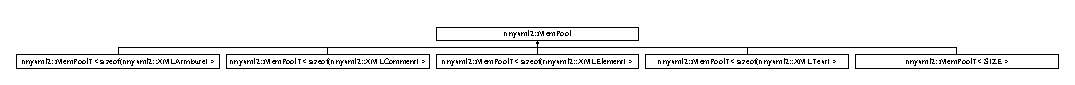
\includegraphics[height=0.691358cm]{classtinyxml2_1_1_mem_pool}
\end{center}
\end{figure}
\subsection*{Public Member Functions}
\begin{DoxyCompactItemize}
\item 
\hypertarget{classtinyxml2_1_1_mem_pool_a0c518d49e3a94bde566f61e13b7240bb}{virtual int {\bfseries Item\-Size} () const =0}\label{classtinyxml2_1_1_mem_pool_a0c518d49e3a94bde566f61e13b7240bb}

\item 
\hypertarget{classtinyxml2_1_1_mem_pool_a4f977b5fed752c0bbfe5295f469d6449}{virtual void $\ast$ {\bfseries Alloc} ()=0}\label{classtinyxml2_1_1_mem_pool_a4f977b5fed752c0bbfe5295f469d6449}

\item 
\hypertarget{classtinyxml2_1_1_mem_pool_a49e3bfac2cba2ebd6776b31e571f64f7}{virtual void {\bfseries Free} (void $\ast$)=0}\label{classtinyxml2_1_1_mem_pool_a49e3bfac2cba2ebd6776b31e571f64f7}

\item 
\hypertarget{classtinyxml2_1_1_mem_pool_ac5804dd1387b2e4de5eef710076a0db1}{virtual void {\bfseries Set\-Tracked} ()=0}\label{classtinyxml2_1_1_mem_pool_ac5804dd1387b2e4de5eef710076a0db1}

\end{DoxyCompactItemize}


The documentation for this class was generated from the following file\-:\begin{DoxyCompactItemize}
\item 
tinyxml2.\-h\end{DoxyCompactItemize}

\hypertarget{classtinyxml2_1_1_mem_pool_t}{\section{tinyxml2\-:\-:Mem\-Pool\-T$<$ S\-I\-Z\-E $>$ Class Template Reference}
\label{classtinyxml2_1_1_mem_pool_t}\index{tinyxml2\-::\-Mem\-Pool\-T$<$ S\-I\-Z\-E $>$@{tinyxml2\-::\-Mem\-Pool\-T$<$ S\-I\-Z\-E $>$}}
}
Inheritance diagram for tinyxml2\-:\-:Mem\-Pool\-T$<$ S\-I\-Z\-E $>$\-:\begin{figure}[H]
\begin{center}
\leavevmode
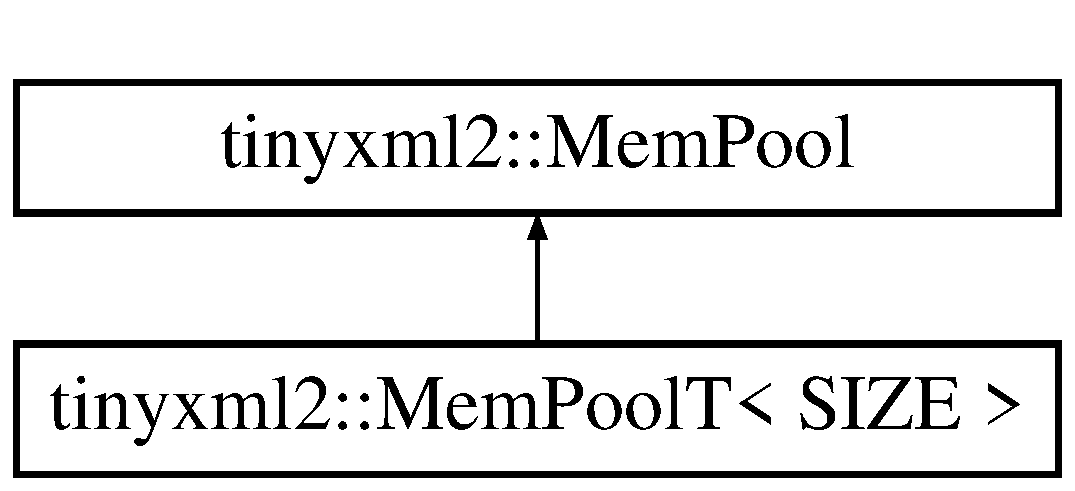
\includegraphics[height=2.000000cm]{classtinyxml2_1_1_mem_pool_t}
\end{center}
\end{figure}
\subsection*{Public Types}
\begin{DoxyCompactItemize}
\item 
enum \{ {\bfseries C\-O\-U\-N\-T} = (4$\ast$1024)/\-S\-I\-Z\-E
 \}
\end{DoxyCompactItemize}
\subsection*{Public Member Functions}
\begin{DoxyCompactItemize}
\item 
\hypertarget{classtinyxml2_1_1_mem_pool_t_a7ec8778fe99f6e332615a703be0b48bc}{virtual int {\bfseries Item\-Size} () const }\label{classtinyxml2_1_1_mem_pool_t_a7ec8778fe99f6e332615a703be0b48bc}

\item 
\hypertarget{classtinyxml2_1_1_mem_pool_t_a56be11b7db6a7ef00db17088a7769aab}{int {\bfseries Current\-Allocs} () const }\label{classtinyxml2_1_1_mem_pool_t_a56be11b7db6a7ef00db17088a7769aab}

\item 
\hypertarget{classtinyxml2_1_1_mem_pool_t_aa9d785a48ffe6ea1be679bab13464486}{virtual void $\ast$ {\bfseries Alloc} ()}\label{classtinyxml2_1_1_mem_pool_t_aa9d785a48ffe6ea1be679bab13464486}

\item 
\hypertarget{classtinyxml2_1_1_mem_pool_t_a4f1a0c434e9e3d7391e5c16ed4ee8c70}{virtual void {\bfseries Free} (void $\ast$mem)}\label{classtinyxml2_1_1_mem_pool_t_a4f1a0c434e9e3d7391e5c16ed4ee8c70}

\item 
\hypertarget{classtinyxml2_1_1_mem_pool_t_a0bc596f271e0f139822c534238b3f244}{void {\bfseries Trace} (const char $\ast$name)}\label{classtinyxml2_1_1_mem_pool_t_a0bc596f271e0f139822c534238b3f244}

\item 
\hypertarget{classtinyxml2_1_1_mem_pool_t_a7798932414916199a1bc0f9c3f368521}{void {\bfseries Set\-Tracked} ()}\label{classtinyxml2_1_1_mem_pool_t_a7798932414916199a1bc0f9c3f368521}

\item 
\hypertarget{classtinyxml2_1_1_mem_pool_t_a524b90d0edeac41964c06510757dce0f}{int {\bfseries Untracked} () const }\label{classtinyxml2_1_1_mem_pool_t_a524b90d0edeac41964c06510757dce0f}

\end{DoxyCompactItemize}


The documentation for this class was generated from the following file\-:\begin{DoxyCompactItemize}
\item 
tinyxml2.\-h\end{DoxyCompactItemize}

\hypertarget{struct_region}{\section{Region Struct Reference}
\label{struct_region}\index{Region@{Region}}
}


a region of the texture atlas  


\subsection*{Public Attributes}
\begin{DoxyCompactItemize}
\item 
\hypertarget{struct_region_ab3a84ba2dfaba1e48bae988a5b0110fc}{float {\bfseries u0}}\label{struct_region_ab3a84ba2dfaba1e48bae988a5b0110fc}

\item 
\hypertarget{struct_region_ae1f101f8c555d1ca72b9c0088d22da58}{float {\bfseries v0}}\label{struct_region_ae1f101f8c555d1ca72b9c0088d22da58}

\item 
\hypertarget{struct_region_ac90f80b38908b321730bebfe13bd1899}{float {\bfseries u1}}\label{struct_region_ac90f80b38908b321730bebfe13bd1899}

\item 
\hypertarget{struct_region_a6c63e8a1907ece81277cdf737f709c7d}{float {\bfseries v1}}\label{struct_region_a6c63e8a1907ece81277cdf737f709c7d}

\item 
\hypertarget{struct_region_a698ecc023295bbb19f7a05729b22d1f3}{int {\bfseries w}}\label{struct_region_a698ecc023295bbb19f7a05729b22d1f3}

\item 
\hypertarget{struct_region_a3be01083660b1aad6276e5406a39b213}{int {\bfseries h}}\label{struct_region_a3be01083660b1aad6276e5406a39b213}

\end{DoxyCompactItemize}


\subsection{Detailed Description}
a region of the texture atlas 

The documentation for this struct was generated from the following file\-:\begin{DoxyCompactItemize}
\item 
Texture\-Atlas.\-cpp\end{DoxyCompactItemize}

\hypertarget{struct_sprite}{\section{Sprite Struct Reference}
\label{struct_sprite}\index{Sprite@{Sprite}}
}


data for a sprite  




{\ttfamily \#include $<$Texture\-Atlas.\-h$>$}

\subsection*{Public Attributes}
\begin{DoxyCompactItemize}
\item 
\hypertarget{struct_sprite_a22e1375f618ebfe6d63fb113fc63c9de}{unsigned int {\bfseries assed\-I\-D}}\label{struct_sprite_a22e1375f618ebfe6d63fb113fc63c9de}

\item 
\hypertarget{struct_sprite_ad5222d1d6d41088ab80cf7e096461799}{float {\bfseries x}}\label{struct_sprite_ad5222d1d6d41088ab80cf7e096461799}

\item 
\hypertarget{struct_sprite_ad09503279ec7c1b96bf67566a917e183}{float {\bfseries y}}\label{struct_sprite_ad09503279ec7c1b96bf67566a917e183}

\item 
\hypertarget{struct_sprite_af3b58d18e88bf5c5dff221f9acffd04d}{float {\bfseries f\-Alpha}}\label{struct_sprite_af3b58d18e88bf5c5dff221f9acffd04d}

\end{DoxyCompactItemize}


\subsection{Detailed Description}
data for a sprite 

The documentation for this struct was generated from the following file\-:\begin{DoxyCompactItemize}
\item 
Texture\-Atlas.\-h\end{DoxyCompactItemize}

\hypertarget{classtinyxml2_1_1_str_pair}{\section{tinyxml2\-:\-:Str\-Pair Class Reference}
\label{classtinyxml2_1_1_str_pair}\index{tinyxml2\-::\-Str\-Pair@{tinyxml2\-::\-Str\-Pair}}
}
\subsection*{Public Types}
\begin{DoxyCompactItemize}
\item 
enum \{ \\*
{\bfseries N\-E\-E\-D\-S\-\_\-\-E\-N\-T\-I\-T\-Y\-\_\-\-P\-R\-O\-C\-E\-S\-S\-I\-N\-G} = 0x01, 
{\bfseries N\-E\-E\-D\-S\-\_\-\-N\-E\-W\-L\-I\-N\-E\-\_\-\-N\-O\-R\-M\-A\-L\-I\-Z\-A\-T\-I\-O\-N} = 0x02, 
{\bfseries C\-O\-L\-L\-A\-P\-S\-E\-\_\-\-W\-H\-I\-T\-E\-S\-P\-A\-C\-E} = 0x04, 
{\bfseries T\-E\-X\-T\-\_\-\-E\-L\-E\-M\-E\-N\-T} = N\-E\-E\-D\-S\-\_\-\-E\-N\-T\-I\-T\-Y\-\_\-\-P\-R\-O\-C\-E\-S\-S\-I\-N\-G $|$ N\-E\-E\-D\-S\-\_\-\-N\-E\-W\-L\-I\-N\-E\-\_\-\-N\-O\-R\-M\-A\-L\-I\-Z\-A\-T\-I\-O\-N, 
\\*
{\bfseries T\-E\-X\-T\-\_\-\-E\-L\-E\-M\-E\-N\-T\-\_\-\-L\-E\-A\-V\-E\-\_\-\-E\-N\-T\-I\-T\-I\-E\-S} = N\-E\-E\-D\-S\-\_\-\-N\-E\-W\-L\-I\-N\-E\-\_\-\-N\-O\-R\-M\-A\-L\-I\-Z\-A\-T\-I\-O\-N, 
{\bfseries A\-T\-T\-R\-I\-B\-U\-T\-E\-\_\-\-N\-A\-M\-E} = 0, 
{\bfseries A\-T\-T\-R\-I\-B\-U\-T\-E\-\_\-\-V\-A\-L\-U\-E} = N\-E\-E\-D\-S\-\_\-\-E\-N\-T\-I\-T\-Y\-\_\-\-P\-R\-O\-C\-E\-S\-S\-I\-N\-G $|$ N\-E\-E\-D\-S\-\_\-\-N\-E\-W\-L\-I\-N\-E\-\_\-\-N\-O\-R\-M\-A\-L\-I\-Z\-A\-T\-I\-O\-N, 
{\bfseries A\-T\-T\-R\-I\-B\-U\-T\-E\-\_\-\-V\-A\-L\-U\-E\-\_\-\-L\-E\-A\-V\-E\-\_\-\-E\-N\-T\-I\-T\-I\-E\-S} = N\-E\-E\-D\-S\-\_\-\-N\-E\-W\-L\-I\-N\-E\-\_\-\-N\-O\-R\-M\-A\-L\-I\-Z\-A\-T\-I\-O\-N, 
\\*
{\bfseries C\-O\-M\-M\-E\-N\-T} = N\-E\-E\-D\-S\-\_\-\-N\-E\-W\-L\-I\-N\-E\-\_\-\-N\-O\-R\-M\-A\-L\-I\-Z\-A\-T\-I\-O\-N
 \}
\end{DoxyCompactItemize}
\subsection*{Public Member Functions}
\begin{DoxyCompactItemize}
\item 
\hypertarget{classtinyxml2_1_1_str_pair_a4f05549373394266a1eecba26813c166}{void {\bfseries Set} (char $\ast$start, char $\ast$end, int flags)}\label{classtinyxml2_1_1_str_pair_a4f05549373394266a1eecba26813c166}

\item 
\hypertarget{classtinyxml2_1_1_str_pair_ad87e3d11330f5e689ba1e7e54c023b57}{const char $\ast$ {\bfseries Get\-Str} ()}\label{classtinyxml2_1_1_str_pair_ad87e3d11330f5e689ba1e7e54c023b57}

\item 
\hypertarget{classtinyxml2_1_1_str_pair_affa1043e73a18f05d5d2faec055725a7}{bool {\bfseries Empty} () const }\label{classtinyxml2_1_1_str_pair_affa1043e73a18f05d5d2faec055725a7}

\item 
\hypertarget{classtinyxml2_1_1_str_pair_a2baf6230e18333e02ab65d0897ee3941}{void {\bfseries Set\-Interned\-Str} (const char $\ast$str)}\label{classtinyxml2_1_1_str_pair_a2baf6230e18333e02ab65d0897ee3941}

\item 
\hypertarget{classtinyxml2_1_1_str_pair_a1f82ec6b5bee35ee7466d8565e43b1de}{void {\bfseries Set\-Str} (const char $\ast$str, int flags=0)}\label{classtinyxml2_1_1_str_pair_a1f82ec6b5bee35ee7466d8565e43b1de}

\item 
\hypertarget{classtinyxml2_1_1_str_pair_ad90521f188e9606a8fbafe5d86fb2246}{char $\ast$ {\bfseries Parse\-Text} (char $\ast$in, const char $\ast$end\-Tag, int str\-Flags)}\label{classtinyxml2_1_1_str_pair_ad90521f188e9606a8fbafe5d86fb2246}

\item 
\hypertarget{classtinyxml2_1_1_str_pair_aa6d8998efceba41d87ec2300c70a6085}{char $\ast$ {\bfseries Parse\-Name} (char $\ast$in)}\label{classtinyxml2_1_1_str_pair_aa6d8998efceba41d87ec2300c70a6085}

\end{DoxyCompactItemize}


The documentation for this class was generated from the following files\-:\begin{DoxyCompactItemize}
\item 
tinyxml2.\-h\item 
tinyxml2.\-cpp\end{DoxyCompactItemize}

\hypertarget{class_texture_atlas}{\section{Texture\-Atlas Class Reference}
\label{class_texture_atlas}\index{Texture\-Atlas@{Texture\-Atlas}}
}


\hyperlink{class_texture_atlas}{Texture\-Atlas} handle the textures and their instances , keeping track of them and upload them to the G\-P\-U.  




{\ttfamily \#include $<$Texture\-Atlas.\-h$>$}

\subsection*{Public Member Functions}
\begin{DoxyCompactItemize}
\item 
\hypertarget{class_texture_atlas_ad38d24295c6a728256392a9f2bcdf8e7}{\hyperlink{class_texture_atlas_ad38d24295c6a728256392a9f2bcdf8e7}{Texture\-Atlas} ()}\label{class_texture_atlas_ad38d24295c6a728256392a9f2bcdf8e7}

\begin{DoxyCompactList}\small\item\em structor \end{DoxyCompactList}\item 
\hypertarget{class_texture_atlas_aed47504c1211eacc876b643e766365d1}{\hyperlink{class_texture_atlas_aed47504c1211eacc876b643e766365d1}{$\sim$\-Texture\-Atlas} ()}\label{class_texture_atlas_aed47504c1211eacc876b643e766365d1}

\begin{DoxyCompactList}\small\item\em brief \end{DoxyCompactList}\item 
\hypertarget{class_texture_atlas_adb753ad8899a9e1045c5cfd84808b3de}{void \hyperlink{class_texture_atlas_adb753ad8899a9e1045c5cfd84808b3de}{Add\-Instance} (const \hyperlink{structking_1_1renderer_1_1_vert}{king\-::renderer\-::\-Vert} $\ast$p\-Vert, unsigned int numpsprite)}\label{class_texture_atlas_adb753ad8899a9e1045c5cfd84808b3de}

\begin{DoxyCompactList}\small\item\em add a texture instance to the render queue. \end{DoxyCompactList}\item 
\hypertarget{class_texture_atlas_a3502f5541a5eee4dd40016570e3d6d22}{void \hyperlink{class_texture_atlas_a3502f5541a5eee4dd40016570e3d6d22}{Add\-Instance} (unsigned int region, float x, float y, float fa\-Alpha)}\label{class_texture_atlas_a3502f5541a5eee4dd40016570e3d6d22}

\begin{DoxyCompactList}\small\item\em add one istance taken from the given region \end{DoxyCompactList}\item 
\hypertarget{class_texture_atlas_a81b2cb15b666a318de3a89532d8bc69c}{void \hyperlink{class_texture_atlas_a81b2cb15b666a318de3a89532d8bc69c}{Add\-Region} (float u0, float v0, float u1, float v1, int w, int h)}\label{class_texture_atlas_a81b2cb15b666a318de3a89532d8bc69c}

\begin{DoxyCompactList}\small\item\em add a texture region to atlas \end{DoxyCompactList}\item 
\hypertarget{class_texture_atlas_a251b652b2fd3a5902ae1bf83d3697429}{void \hyperlink{class_texture_atlas_a251b652b2fd3a5902ae1bf83d3697429}{Load\-Texture} (const char $\ast$p\-Data)}\label{class_texture_atlas_a251b652b2fd3a5902ae1bf83d3697429}

\begin{DoxyCompactList}\small\item\em load textture \end{DoxyCompactList}\item 
\hypertarget{class_texture_atlas_ad52320227c97485cf77ffa62c167b428}{void \hyperlink{class_texture_atlas_ad52320227c97485cf77ffa62c167b428}{Draw} (unsigned int shader)}\label{class_texture_atlas_ad52320227c97485cf77ffa62c167b428}

\begin{DoxyCompactList}\small\item\em issue draw \end{DoxyCompactList}\item 
\hypertarget{class_texture_atlas_ab864214908340929d817bbe38d96a828}{void \hyperlink{class_texture_atlas_ab864214908340929d817bbe38d96a828}{Flush} ()}\label{class_texture_atlas_ab864214908340929d817bbe38d96a828}

\begin{DoxyCompactList}\small\item\em the data \end{DoxyCompactList}\end{DoxyCompactItemize}
\subsection*{Static Public Attributes}
\begin{DoxyCompactItemize}
\item 
\hypertarget{class_texture_atlas_a2f7a634462064e7715e58eb15fb13bdd}{static const int \hyperlink{class_texture_atlas_a2f7a634462064e7715e58eb15fb13bdd}{k\-Max\-Instances} = 1024}\label{class_texture_atlas_a2f7a634462064e7715e58eb15fb13bdd}

\begin{DoxyCompactList}\small\item\em brief max numer of instance supported \end{DoxyCompactList}\item 
\hypertarget{class_texture_atlas_a94887a34f2e8a2b3ffa794e3561619d4}{static const int \hyperlink{class_texture_atlas_a94887a34f2e8a2b3ffa794e3561619d4}{k\-Max\-Sprite\-Per\-Atlas} = 256}\label{class_texture_atlas_a94887a34f2e8a2b3ffa794e3561619d4}

\begin{DoxyCompactList}\small\item\em define the maximon number of sprite per atlas \end{DoxyCompactList}\end{DoxyCompactItemize}


\subsection{Detailed Description}
\hyperlink{class_texture_atlas}{Texture\-Atlas} handle the textures and their instances , keeping track of them and upload them to the G\-P\-U. 

The documentation for this class was generated from the following files\-:\begin{DoxyCompactItemize}
\item 
Texture\-Atlas.\-h\item 
Texture\-Atlas.\-cpp\end{DoxyCompactItemize}

\hypertarget{struct_texture_atlas_data}{\section{Texture\-Atlas\-Data Struct Reference}
\label{struct_texture_atlas_data}\index{Texture\-Atlas\-Data@{Texture\-Atlas\-Data}}
}


brief pimpl \-: define internal state here to make the interface more clear and avoid depencies  


\subsection*{Public Attributes}
\begin{DoxyCompactItemize}
\item 
\hypertarget{struct_texture_atlas_data_af9945277a693c03e09fbb25d4f832575}{unsigned int {\bfseries num\-Instance}}\label{struct_texture_atlas_data_af9945277a693c03e09fbb25d4f832575}

\item 
\hypertarget{struct_texture_atlas_data_a698b1201494e4594c1e61d8eaa89c7bf}{unsigned int {\bfseries num\-Region}}\label{struct_texture_atlas_data_a698b1201494e4594c1e61d8eaa89c7bf}

\item 
\hypertarget{struct_texture_atlas_data_abceb90af2ece1bd3f50b68fcecce7a52}{\hyperlink{class_linear_allocator}{Linear\-Allocator} {\bfseries v\-Buffer}}\label{struct_texture_atlas_data_abceb90af2ece1bd3f50b68fcecce7a52}

\item 
\hypertarget{struct_texture_atlas_data_aecd18978b18c6b35f6a3ce7dd0ade997}{\hyperlink{class_linear_allocator}{Linear\-Allocator} {\bfseries i\-Buffer}}\label{struct_texture_atlas_data_aecd18978b18c6b35f6a3ce7dd0ade997}

\item 
\hypertarget{struct_texture_atlas_data_a0eb0a7570f865e168395124b953cfcb0}{unsigned int {\bfseries i\-Buffer\-Id}}\label{struct_texture_atlas_data_a0eb0a7570f865e168395124b953cfcb0}

\item 
\hypertarget{struct_texture_atlas_data_afa1ad1ba165e54a8ab31e0f41d288556}{unsigned int {\bfseries v\-Buffer\-Id}}\label{struct_texture_atlas_data_afa1ad1ba165e54a8ab31e0f41d288556}

\item 
\hypertarget{struct_texture_atlas_data_a0c4f8afb74523c3224d44ffe658e2137}{unsigned int {\bfseries v\-Shader\-Id}}\label{struct_texture_atlas_data_a0c4f8afb74523c3224d44ffe658e2137}

\item 
\hypertarget{struct_texture_atlas_data_af916eb64927963704582b4f0fca67bff}{unsigned int {\bfseries v\-Texture\-Id}}\label{struct_texture_atlas_data_af916eb64927963704582b4f0fca67bff}

\item 
\hypertarget{struct_texture_atlas_data_a9363a9f2dddbfaf0b8d77a316ee7922b}{\hyperlink{struct_region}{Region} {\bfseries a\-Regions} \mbox{[}\hyperlink{class_texture_atlas_a94887a34f2e8a2b3ffa794e3561619d4}{Texture\-Atlas\-::k\-Max\-Sprite\-Per\-Atlas}\mbox{]}}\label{struct_texture_atlas_data_a9363a9f2dddbfaf0b8d77a316ee7922b}

\end{DoxyCompactItemize}


\subsection{Detailed Description}
brief pimpl \-: define internal state here to make the interface more clear and avoid depencies 

The documentation for this struct was generated from the following file\-:\begin{DoxyCompactItemize}
\item 
Texture\-Atlas.\-cpp\end{DoxyCompactItemize}

\hypertarget{class_t_link}{\section{T\-Link$<$ T $>$ Class Template Reference}
\label{class_t_link}\index{T\-Link$<$ T $>$@{T\-Link$<$ T $>$}}
}
\subsection*{Public Member Functions}
\begin{DoxyCompactItemize}
\item 
\hypertarget{class_t_link_aa01e1ccd6b7846016012a5343224c1b5}{bool {\bfseries Is\-Linked} () const }\label{class_t_link_aa01e1ccd6b7846016012a5343224c1b5}

\item 
\hypertarget{class_t_link_a14724694f16ea9d88062e3f14d139f14}{void {\bfseries Unlink} ()}\label{class_t_link_a14724694f16ea9d88062e3f14d139f14}

\item 
\hypertarget{class_t_link_a52dd2245c7c585d9bed1f30d12698cb7}{T $\ast$ {\bfseries Prev} ()}\label{class_t_link_a52dd2245c7c585d9bed1f30d12698cb7}

\item 
\hypertarget{class_t_link_ac554775ff4a03d9910df8a02d64679d9}{T $\ast$ {\bfseries Next} ()}\label{class_t_link_ac554775ff4a03d9910df8a02d64679d9}

\item 
\hypertarget{class_t_link_a66d75afd6f0c37ad08bc670f6ca4aa58}{const T $\ast$ {\bfseries Prev} () const }\label{class_t_link_a66d75afd6f0c37ad08bc670f6ca4aa58}

\item 
\hypertarget{class_t_link_a9b4cc1c1ae47207eda1513bd0a0209b5}{const T $\ast$ {\bfseries Next} () const }\label{class_t_link_a9b4cc1c1ae47207eda1513bd0a0209b5}

\item 
\hypertarget{class_t_link_ac110b19a42fdb07d693821a26ba23e73}{{\bfseries T\-Link} (size\-\_\-t offset)}\label{class_t_link_ac110b19a42fdb07d693821a26ba23e73}

\item 
\hypertarget{class_t_link_a67cf76748fc80be33887a3d4bf1cb7cb}{void {\bfseries Set\-Offset} (size\-\_\-t offset)}\label{class_t_link_a67cf76748fc80be33887a3d4bf1cb7cb}

\item 
\hypertarget{class_t_link_a5e58431627debb2040c18c04f3642694}{\hyperlink{class_t_link}{T\-Link}$<$ T $>$ $\ast$ {\bfseries Next\-Link} ()}\label{class_t_link_a5e58431627debb2040c18c04f3642694}

\item 
\hypertarget{class_t_link_ae6f2c9f1ceaed42ffab535ed12d78088}{\hyperlink{class_t_link}{T\-Link}$<$ T $>$ $\ast$ {\bfseries Prev\-Link} ()}\label{class_t_link_ae6f2c9f1ceaed42ffab535ed12d78088}

\item 
\hypertarget{class_t_link_a24c6e9c3d7689fa7616ce8765658bfb1}{void {\bfseries Insert\-Before} (T $\ast$node, \hyperlink{class_t_link}{T\-Link}$<$ T $>$ $\ast$next\-Link)}\label{class_t_link_a24c6e9c3d7689fa7616ce8765658bfb1}

\item 
\hypertarget{class_t_link_af2d24026f2beae7d09b32976d72fbc91}{void {\bfseries Insert\-After} (T $\ast$node, \hyperlink{class_t_link}{T\-Link}$<$ T $>$ $\ast$prev\-Link)}\label{class_t_link_af2d24026f2beae7d09b32976d72fbc91}

\end{DoxyCompactItemize}


The documentation for this class was generated from the following file\-:\begin{DoxyCompactItemize}
\item 
List.\-h\end{DoxyCompactItemize}

\hypertarget{class_t_list}{\section{T\-List$<$ T $>$ Class Template Reference}
\label{class_t_list}\index{T\-List$<$ T $>$@{T\-List$<$ T $>$}}
}
Inheritance diagram for T\-List$<$ T $>$\-:\begin{figure}[H]
\begin{center}
\leavevmode
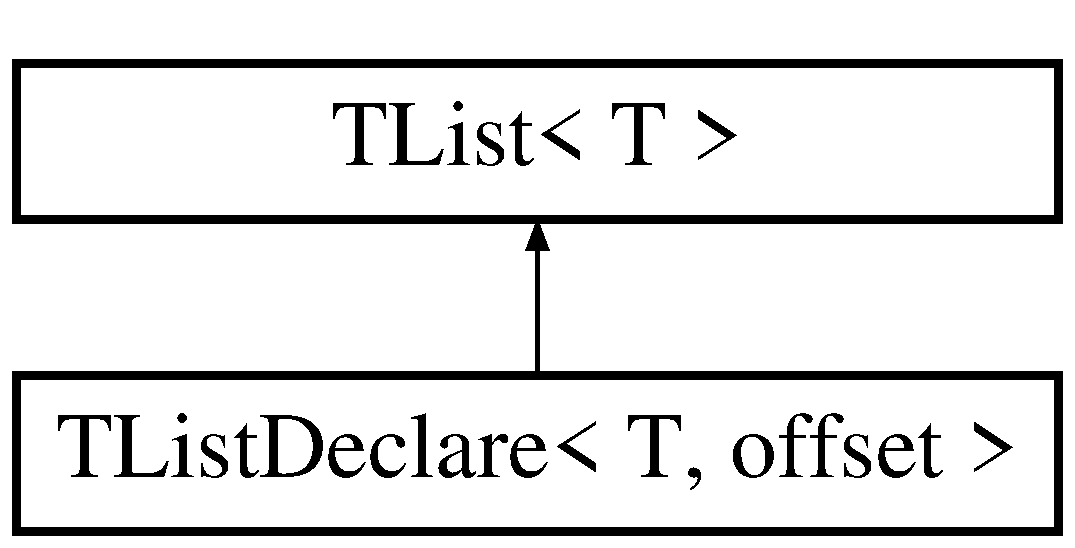
\includegraphics[height=2.000000cm]{class_t_list}
\end{center}
\end{figure}
\subsection*{Public Member Functions}
\begin{DoxyCompactItemize}
\item 
\hypertarget{class_t_list_a2944c214a30f44ea70a18cc3119fe5e8}{bool {\bfseries Empty} () const }\label{class_t_list_a2944c214a30f44ea70a18cc3119fe5e8}

\item 
\hypertarget{class_t_list_a35523aa9323bdecc29cdf532f664ce4b}{void {\bfseries Unlink\-All} ()}\label{class_t_list_a35523aa9323bdecc29cdf532f664ce4b}

\item 
\hypertarget{class_t_list_a75f2706f45be3121725c8b5d188ccc4e}{void {\bfseries Delete\-All} ()}\label{class_t_list_a75f2706f45be3121725c8b5d188ccc4e}

\item 
\hypertarget{class_t_list_a84b55b38d4bf09fc4989596dfae53f05}{T $\ast$ {\bfseries Head} ()}\label{class_t_list_a84b55b38d4bf09fc4989596dfae53f05}

\item 
\hypertarget{class_t_list_a2cfaae525a445b323901fc693d0f87ab}{T $\ast$ {\bfseries Tail} ()}\label{class_t_list_a2cfaae525a445b323901fc693d0f87ab}

\item 
\hypertarget{class_t_list_ac60011fb6f5d53c36dac5864b7653a92}{const T $\ast$ {\bfseries Head} () const }\label{class_t_list_ac60011fb6f5d53c36dac5864b7653a92}

\item 
\hypertarget{class_t_list_ad93c3c6b83afbe1c0821bb23c9a4f974}{const T $\ast$ {\bfseries Tail} () const }\label{class_t_list_ad93c3c6b83afbe1c0821bb23c9a4f974}

\item 
\hypertarget{class_t_list_ae747a3c922486b6bd4b6c334ced276c6}{T $\ast$ {\bfseries Prev} (T $\ast$node)}\label{class_t_list_ae747a3c922486b6bd4b6c334ced276c6}

\item 
\hypertarget{class_t_list_ac44a19580c48820ec487a9aa3324dca6}{T $\ast$ {\bfseries Next} (T $\ast$node)}\label{class_t_list_ac44a19580c48820ec487a9aa3324dca6}

\item 
\hypertarget{class_t_list_ad6577416af27d88bdcceae6c46a7ad57}{const T $\ast$ {\bfseries Prev} (const T $\ast$node) const }\label{class_t_list_ad6577416af27d88bdcceae6c46a7ad57}

\item 
\hypertarget{class_t_list_a7b23c3330ad45d8e9bf853701eb39904}{const T $\ast$ {\bfseries Next} (const T $\ast$node) const }\label{class_t_list_a7b23c3330ad45d8e9bf853701eb39904}

\item 
\hypertarget{class_t_list_aabbc9a08cf4efc5ad4ee0c164cf3cd57}{void {\bfseries Insert\-Head} (T $\ast$node)}\label{class_t_list_aabbc9a08cf4efc5ad4ee0c164cf3cd57}

\item 
\hypertarget{class_t_list_abe2b07c26d4b39c01c46bb4acea28aca}{void {\bfseries Insert\-Tail} (T $\ast$node)}\label{class_t_list_abe2b07c26d4b39c01c46bb4acea28aca}

\item 
\hypertarget{class_t_list_a9c838087f0a605443c47020a9ed35f81}{void {\bfseries Insert\-Before} (T $\ast$node, T $\ast$before)}\label{class_t_list_a9c838087f0a605443c47020a9ed35f81}

\item 
\hypertarget{class_t_list_a817600eff42678aa9f12f5f4760f1c05}{void {\bfseries Insert\-After} (T $\ast$node, T $\ast$after)}\label{class_t_list_a817600eff42678aa9f12f5f4760f1c05}

\end{DoxyCompactItemize}
\subsection*{Friends}
\begin{DoxyCompactItemize}
\item 
\hypertarget{class_t_list_af0be59228d62dee9c5a50dad4d79927a}{{\footnotesize template$<$class T , size\-\_\-t offset$>$ }\\class {\bfseries T\-List\-Declare}}\label{class_t_list_af0be59228d62dee9c5a50dad4d79927a}

\end{DoxyCompactItemize}


The documentation for this class was generated from the following file\-:\begin{DoxyCompactItemize}
\item 
List.\-h\end{DoxyCompactItemize}

\hypertarget{class_t_list_declare}{\section{T\-List\-Declare$<$ T, offset $>$ Class Template Reference}
\label{class_t_list_declare}\index{T\-List\-Declare$<$ T, offset $>$@{T\-List\-Declare$<$ T, offset $>$}}
}
Inheritance diagram for T\-List\-Declare$<$ T, offset $>$\-:\begin{figure}[H]
\begin{center}
\leavevmode
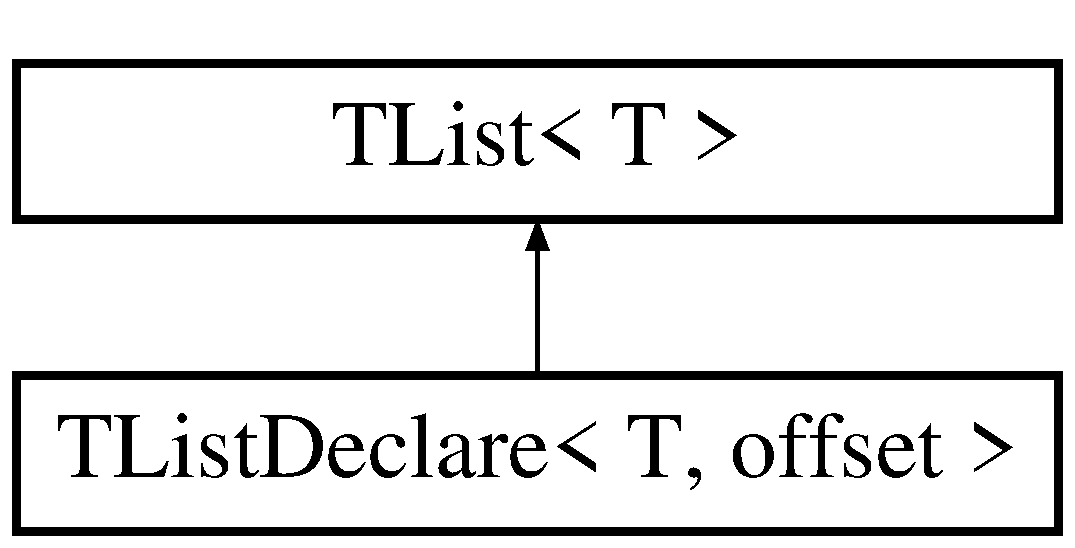
\includegraphics[height=2.000000cm]{class_t_list_declare}
\end{center}
\end{figure}
\subsection*{Additional Inherited Members}


The documentation for this class was generated from the following file\-:\begin{DoxyCompactItemize}
\item 
List.\-h\end{DoxyCompactItemize}

\hypertarget{structking_1_1renderer_1_1_vert}{\section{king\-:\-:renderer\-:\-:Vert Struct Reference}
\label{structking_1_1renderer_1_1_vert}\index{king\-::renderer\-::\-Vert@{king\-::renderer\-::\-Vert}}
}
\subsection*{Public Attributes}
\begin{DoxyCompactItemize}
\item 
\hypertarget{structking_1_1renderer_1_1_vert_a6bddfcdfce0fd66cdf83bab10cb022f8}{float {\bfseries v\-Pos} \mbox{[}3\mbox{]}}\label{structking_1_1renderer_1_1_vert_a6bddfcdfce0fd66cdf83bab10cb022f8}

\item 
\hypertarget{structking_1_1renderer_1_1_vert_a9c0263b6a4b1ab8038827f5568f83085}{float {\bfseries uv} \mbox{[}2\mbox{]}}\label{structking_1_1renderer_1_1_vert_a9c0263b6a4b1ab8038827f5568f83085}

\end{DoxyCompactItemize}


The documentation for this struct was generated from the following file\-:\begin{DoxyCompactItemize}
\item 
Renderer.\-h\end{DoxyCompactItemize}

\hypertarget{classtinyxml2_1_1_x_m_l_attribute}{\section{tinyxml2\-:\-:X\-M\-L\-Attribute Class Reference}
\label{classtinyxml2_1_1_x_m_l_attribute}\index{tinyxml2\-::\-X\-M\-L\-Attribute@{tinyxml2\-::\-X\-M\-L\-Attribute}}
}


{\ttfamily \#include $<$tinyxml2.\-h$>$}

\subsection*{Public Member Functions}
\begin{DoxyCompactItemize}
\item 
\hypertarget{classtinyxml2_1_1_x_m_l_attribute_a631990ac0d176e38fc291b17b295a62d}{const char $\ast$ \hyperlink{classtinyxml2_1_1_x_m_l_attribute_a631990ac0d176e38fc291b17b295a62d}{Name} () const }\label{classtinyxml2_1_1_x_m_l_attribute_a631990ac0d176e38fc291b17b295a62d}

\begin{DoxyCompactList}\small\item\em The name of the attribute. \end{DoxyCompactList}\item 
\hypertarget{classtinyxml2_1_1_x_m_l_attribute_adf884db24f469f8a99a14ae786d4ddd7}{const char $\ast$ \hyperlink{classtinyxml2_1_1_x_m_l_attribute_adf884db24f469f8a99a14ae786d4ddd7}{Value} () const }\label{classtinyxml2_1_1_x_m_l_attribute_adf884db24f469f8a99a14ae786d4ddd7}

\begin{DoxyCompactList}\small\item\em The value of the attribute. \end{DoxyCompactList}\item 
\hypertarget{classtinyxml2_1_1_x_m_l_attribute_a7fd852d6185af90361ec1bc9a7681ad6}{const \hyperlink{classtinyxml2_1_1_x_m_l_attribute}{X\-M\-L\-Attribute} $\ast$ \hyperlink{classtinyxml2_1_1_x_m_l_attribute_a7fd852d6185af90361ec1bc9a7681ad6}{Next} () const }\label{classtinyxml2_1_1_x_m_l_attribute_a7fd852d6185af90361ec1bc9a7681ad6}

\begin{DoxyCompactList}\small\item\em The next attribute in the list. \end{DoxyCompactList}\item 
int \hyperlink{classtinyxml2_1_1_x_m_l_attribute_a949d02a5888092cc68c1e29185301863}{Int\-Value} () const 
\item 
\hypertarget{classtinyxml2_1_1_x_m_l_attribute_a4c7a179907836a136d1ce5acbe53389d}{unsigned \hyperlink{classtinyxml2_1_1_x_m_l_attribute_a4c7a179907836a136d1ce5acbe53389d}{Unsigned\-Value} () const }\label{classtinyxml2_1_1_x_m_l_attribute_a4c7a179907836a136d1ce5acbe53389d}

\begin{DoxyCompactList}\small\item\em Query as an unsigned integer. See \hyperlink{classtinyxml2_1_1_x_m_l_attribute_a949d02a5888092cc68c1e29185301863}{Int\-Value()} \end{DoxyCompactList}\item 
\hypertarget{classtinyxml2_1_1_x_m_l_attribute_afb444b7a12527f836aa161b54b2f7ce7}{bool \hyperlink{classtinyxml2_1_1_x_m_l_attribute_afb444b7a12527f836aa161b54b2f7ce7}{Bool\-Value} () const }\label{classtinyxml2_1_1_x_m_l_attribute_afb444b7a12527f836aa161b54b2f7ce7}

\begin{DoxyCompactList}\small\item\em Query as a boolean. See \hyperlink{classtinyxml2_1_1_x_m_l_attribute_a949d02a5888092cc68c1e29185301863}{Int\-Value()} \end{DoxyCompactList}\item 
\hypertarget{classtinyxml2_1_1_x_m_l_attribute_a336153e5aa1b7ccd6502fc249bfb3fd7}{double \hyperlink{classtinyxml2_1_1_x_m_l_attribute_a336153e5aa1b7ccd6502fc249bfb3fd7}{Double\-Value} () const }\label{classtinyxml2_1_1_x_m_l_attribute_a336153e5aa1b7ccd6502fc249bfb3fd7}

\begin{DoxyCompactList}\small\item\em Query as a double. See \hyperlink{classtinyxml2_1_1_x_m_l_attribute_a949d02a5888092cc68c1e29185301863}{Int\-Value()} \end{DoxyCompactList}\item 
\hypertarget{classtinyxml2_1_1_x_m_l_attribute_ae3d51ff98eacc1dc46efcfdaee5c84ad}{float \hyperlink{classtinyxml2_1_1_x_m_l_attribute_ae3d51ff98eacc1dc46efcfdaee5c84ad}{Float\-Value} () const }\label{classtinyxml2_1_1_x_m_l_attribute_ae3d51ff98eacc1dc46efcfdaee5c84ad}

\begin{DoxyCompactList}\small\item\em Query as a float. See \hyperlink{classtinyxml2_1_1_x_m_l_attribute_a949d02a5888092cc68c1e29185301863}{Int\-Value()} \end{DoxyCompactList}\item 
X\-M\-L\-Error \hyperlink{classtinyxml2_1_1_x_m_l_attribute_ad510a83c4ff2755844bb250b125d28ff}{Query\-Int\-Value} (int $\ast$value) const 
\item 
\hypertarget{classtinyxml2_1_1_x_m_l_attribute_ac93f5981adfd62ac4ea76bfa668ee2b4}{X\-M\-L\-Error \hyperlink{classtinyxml2_1_1_x_m_l_attribute_ac93f5981adfd62ac4ea76bfa668ee2b4}{Query\-Unsigned\-Value} (unsigned int $\ast$value) const }\label{classtinyxml2_1_1_x_m_l_attribute_ac93f5981adfd62ac4ea76bfa668ee2b4}

\begin{DoxyCompactList}\small\item\em See Query\-Int\-Value. \end{DoxyCompactList}\item 
\hypertarget{classtinyxml2_1_1_x_m_l_attribute_a9e9b94369f182df72aaac9acd04afead}{X\-M\-L\-Error \hyperlink{classtinyxml2_1_1_x_m_l_attribute_a9e9b94369f182df72aaac9acd04afead}{Query\-Bool\-Value} (bool $\ast$value) const }\label{classtinyxml2_1_1_x_m_l_attribute_a9e9b94369f182df72aaac9acd04afead}

\begin{DoxyCompactList}\small\item\em See Query\-Int\-Value. \end{DoxyCompactList}\item 
\hypertarget{classtinyxml2_1_1_x_m_l_attribute_a0872c05edea2a7cde4bd96c1e9cb2fc4}{X\-M\-L\-Error \hyperlink{classtinyxml2_1_1_x_m_l_attribute_a0872c05edea2a7cde4bd96c1e9cb2fc4}{Query\-Double\-Value} (double $\ast$value) const }\label{classtinyxml2_1_1_x_m_l_attribute_a0872c05edea2a7cde4bd96c1e9cb2fc4}

\begin{DoxyCompactList}\small\item\em See Query\-Int\-Value. \end{DoxyCompactList}\item 
\hypertarget{classtinyxml2_1_1_x_m_l_attribute_afb254627c296d1d70b755397d32fece8}{X\-M\-L\-Error \hyperlink{classtinyxml2_1_1_x_m_l_attribute_afb254627c296d1d70b755397d32fece8}{Query\-Float\-Value} (float $\ast$value) const }\label{classtinyxml2_1_1_x_m_l_attribute_afb254627c296d1d70b755397d32fece8}

\begin{DoxyCompactList}\small\item\em See Query\-Int\-Value. \end{DoxyCompactList}\item 
\hypertarget{classtinyxml2_1_1_x_m_l_attribute_a406d2c4a13c7af99a65edb59dd9f7581}{void \hyperlink{classtinyxml2_1_1_x_m_l_attribute_a406d2c4a13c7af99a65edb59dd9f7581}{Set\-Attribute} (const char $\ast$value)}\label{classtinyxml2_1_1_x_m_l_attribute_a406d2c4a13c7af99a65edb59dd9f7581}

\begin{DoxyCompactList}\small\item\em Set the attribute to a string value. \end{DoxyCompactList}\item 
\hypertarget{classtinyxml2_1_1_x_m_l_attribute_ad86d7d7058d76761c3a80662566a57e5}{void \hyperlink{classtinyxml2_1_1_x_m_l_attribute_ad86d7d7058d76761c3a80662566a57e5}{Set\-Attribute} (int value)}\label{classtinyxml2_1_1_x_m_l_attribute_ad86d7d7058d76761c3a80662566a57e5}

\begin{DoxyCompactList}\small\item\em Set the attribute to value. \end{DoxyCompactList}\item 
\hypertarget{classtinyxml2_1_1_x_m_l_attribute_ae70468c0f6df2748ba3529c716999fae}{void \hyperlink{classtinyxml2_1_1_x_m_l_attribute_ae70468c0f6df2748ba3529c716999fae}{Set\-Attribute} (unsigned value)}\label{classtinyxml2_1_1_x_m_l_attribute_ae70468c0f6df2748ba3529c716999fae}

\begin{DoxyCompactList}\small\item\em Set the attribute to value. \end{DoxyCompactList}\item 
\hypertarget{classtinyxml2_1_1_x_m_l_attribute_ab3516def4fe058fe328f2b89fc2d77da}{void \hyperlink{classtinyxml2_1_1_x_m_l_attribute_ab3516def4fe058fe328f2b89fc2d77da}{Set\-Attribute} (bool value)}\label{classtinyxml2_1_1_x_m_l_attribute_ab3516def4fe058fe328f2b89fc2d77da}

\begin{DoxyCompactList}\small\item\em Set the attribute to value. \end{DoxyCompactList}\item 
\hypertarget{classtinyxml2_1_1_x_m_l_attribute_a9a65ab3147abe8ccbbd373ce8791e818}{void \hyperlink{classtinyxml2_1_1_x_m_l_attribute_a9a65ab3147abe8ccbbd373ce8791e818}{Set\-Attribute} (double value)}\label{classtinyxml2_1_1_x_m_l_attribute_a9a65ab3147abe8ccbbd373ce8791e818}

\begin{DoxyCompactList}\small\item\em Set the attribute to value. \end{DoxyCompactList}\item 
\hypertarget{classtinyxml2_1_1_x_m_l_attribute_ae95e843313aaf5d56c32530b6456df02}{void \hyperlink{classtinyxml2_1_1_x_m_l_attribute_ae95e843313aaf5d56c32530b6456df02}{Set\-Attribute} (float value)}\label{classtinyxml2_1_1_x_m_l_attribute_ae95e843313aaf5d56c32530b6456df02}

\begin{DoxyCompactList}\small\item\em Set the attribute to value. \end{DoxyCompactList}\end{DoxyCompactItemize}
\subsection*{Friends}
\begin{DoxyCompactItemize}
\item 
\hypertarget{classtinyxml2_1_1_x_m_l_attribute_ac2fba9b6e452829dd892f7392c24e0eb}{class {\bfseries X\-M\-L\-Element}}\label{classtinyxml2_1_1_x_m_l_attribute_ac2fba9b6e452829dd892f7392c24e0eb}

\end{DoxyCompactItemize}


\subsection{Detailed Description}
An attribute is a name-\/value pair. Elements have an arbitrary number of attributes, each with a unique name.

\begin{DoxyNote}{Note}
The attributes are not X\-M\-L\-Nodes. You may only query the \hyperlink{classtinyxml2_1_1_x_m_l_attribute_a7fd852d6185af90361ec1bc9a7681ad6}{Next()} attribute in a list. 
\end{DoxyNote}


\subsection{Member Function Documentation}
\hypertarget{classtinyxml2_1_1_x_m_l_attribute_a949d02a5888092cc68c1e29185301863}{\index{tinyxml2\-::\-X\-M\-L\-Attribute@{tinyxml2\-::\-X\-M\-L\-Attribute}!Int\-Value@{Int\-Value}}
\index{Int\-Value@{Int\-Value}!tinyxml2::XMLAttribute@{tinyxml2\-::\-X\-M\-L\-Attribute}}
\subsubsection[{Int\-Value}]{\setlength{\rightskip}{0pt plus 5cm}int tinyxml2\-::\-X\-M\-L\-Attribute\-::\-Int\-Value (
\begin{DoxyParamCaption}
{}
\end{DoxyParamCaption}
) const\hspace{0.3cm}{\ttfamily [inline]}}}\label{classtinyxml2_1_1_x_m_l_attribute_a949d02a5888092cc68c1e29185301863}
Int\-Value interprets the attribute as an integer, and returns the value. If the value isn't an integer, 0 will be returned. There is no error checking; use \hyperlink{classtinyxml2_1_1_x_m_l_attribute_ad510a83c4ff2755844bb250b125d28ff}{Query\-Int\-Value()} if you need error checking. \hypertarget{classtinyxml2_1_1_x_m_l_attribute_ad510a83c4ff2755844bb250b125d28ff}{\index{tinyxml2\-::\-X\-M\-L\-Attribute@{tinyxml2\-::\-X\-M\-L\-Attribute}!Query\-Int\-Value@{Query\-Int\-Value}}
\index{Query\-Int\-Value@{Query\-Int\-Value}!tinyxml2::XMLAttribute@{tinyxml2\-::\-X\-M\-L\-Attribute}}
\subsubsection[{Query\-Int\-Value}]{\setlength{\rightskip}{0pt plus 5cm}X\-M\-L\-Error tinyxml2\-::\-X\-M\-L\-Attribute\-::\-Query\-Int\-Value (
\begin{DoxyParamCaption}
\item[{int $\ast$}]{value}
\end{DoxyParamCaption}
) const}}\label{classtinyxml2_1_1_x_m_l_attribute_ad510a83c4ff2755844bb250b125d28ff}
Query\-Int\-Value interprets the attribute as an integer, and returns the value in the provided parameter. The function will return X\-M\-L\-\_\-\-N\-O\-\_\-\-E\-R\-R\-O\-R on success, and X\-M\-L\-\_\-\-W\-R\-O\-N\-G\-\_\-\-A\-T\-T\-R\-I\-B\-U\-T\-E\-\_\-\-T\-Y\-P\-E if the conversion is not successful. 

The documentation for this class was generated from the following files\-:\begin{DoxyCompactItemize}
\item 
tinyxml2.\-h\item 
tinyxml2.\-cpp\end{DoxyCompactItemize}

\hypertarget{classtinyxml2_1_1_x_m_l_comment}{\section{tinyxml2\-:\-:X\-M\-L\-Comment Class Reference}
\label{classtinyxml2_1_1_x_m_l_comment}\index{tinyxml2\-::\-X\-M\-L\-Comment@{tinyxml2\-::\-X\-M\-L\-Comment}}
}


{\ttfamily \#include $<$tinyxml2.\-h$>$}

Inheritance diagram for tinyxml2\-:\-:X\-M\-L\-Comment\-:\begin{figure}[H]
\begin{center}
\leavevmode
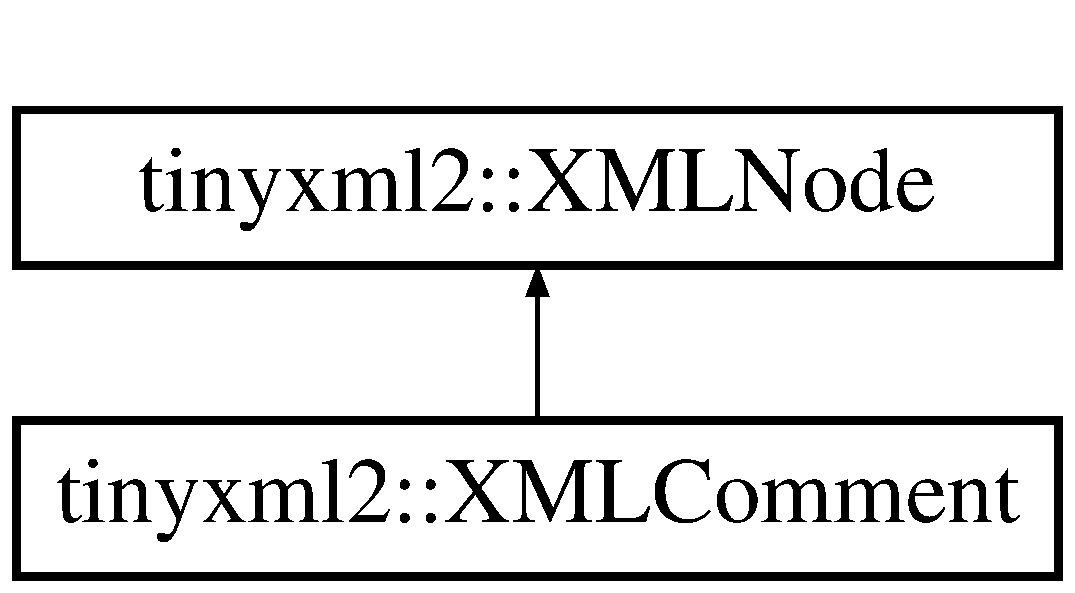
\includegraphics[height=2.000000cm]{classtinyxml2_1_1_x_m_l_comment}
\end{center}
\end{figure}
\subsection*{Public Member Functions}
\begin{DoxyCompactItemize}
\item 
\hypertarget{classtinyxml2_1_1_x_m_l_comment_a8093e1dc8a34fa446d9dc3fde0e6c0ee}{virtual \hyperlink{classtinyxml2_1_1_x_m_l_comment}{X\-M\-L\-Comment} $\ast$ \hyperlink{classtinyxml2_1_1_x_m_l_comment_a8093e1dc8a34fa446d9dc3fde0e6c0ee}{To\-Comment} ()}\label{classtinyxml2_1_1_x_m_l_comment_a8093e1dc8a34fa446d9dc3fde0e6c0ee}

\begin{DoxyCompactList}\small\item\em Safely cast to a Comment, or null. \end{DoxyCompactList}\item 
\hypertarget{classtinyxml2_1_1_x_m_l_comment_a422aabac22de7d9c9cad130897dd8b1c}{virtual const \hyperlink{classtinyxml2_1_1_x_m_l_comment}{X\-M\-L\-Comment} $\ast$ {\bfseries To\-Comment} () const }\label{classtinyxml2_1_1_x_m_l_comment_a422aabac22de7d9c9cad130897dd8b1c}

\item 
virtual bool \hyperlink{classtinyxml2_1_1_x_m_l_comment_aa382b1be6a8b0650c16a2d88bb499335}{Accept} (\hyperlink{classtinyxml2_1_1_x_m_l_visitor}{X\-M\-L\-Visitor} $\ast$visitor) const 
\item 
\hypertarget{classtinyxml2_1_1_x_m_l_comment_aa6ab35c3bb1c1840371dc32a2040c57f}{char $\ast$ {\bfseries Parse\-Deep} (char $\ast$, \hyperlink{classtinyxml2_1_1_str_pair}{Str\-Pair} $\ast$end\-Tag)}\label{classtinyxml2_1_1_x_m_l_comment_aa6ab35c3bb1c1840371dc32a2040c57f}

\item 
virtual \hyperlink{classtinyxml2_1_1_x_m_l_node}{X\-M\-L\-Node} $\ast$ \hyperlink{classtinyxml2_1_1_x_m_l_comment_a90bb60193a691b484f5e1b487857016d}{Shallow\-Clone} (\hyperlink{classtinyxml2_1_1_x_m_l_document}{X\-M\-L\-Document} $\ast$document) const 
\item 
virtual bool \hyperlink{classtinyxml2_1_1_x_m_l_comment_a2d9f26757b0018fce933e74420cda22a}{Shallow\-Equal} (const \hyperlink{classtinyxml2_1_1_x_m_l_node}{X\-M\-L\-Node} $\ast$compare) const 
\end{DoxyCompactItemize}
\subsection*{Protected Member Functions}
\begin{DoxyCompactItemize}
\item 
\hypertarget{classtinyxml2_1_1_x_m_l_comment_ae6463adc3edd93a8e5a9b2b7e99cdf91}{{\bfseries X\-M\-L\-Comment} (\hyperlink{classtinyxml2_1_1_x_m_l_document}{X\-M\-L\-Document} $\ast$doc)}\label{classtinyxml2_1_1_x_m_l_comment_ae6463adc3edd93a8e5a9b2b7e99cdf91}

\item 
\hypertarget{classtinyxml2_1_1_x_m_l_comment_aa0a9aae0850ac0e70d3cd20f6cb44447}{{\bfseries X\-M\-L\-Comment} (const \hyperlink{classtinyxml2_1_1_x_m_l_comment}{X\-M\-L\-Comment} \&)}\label{classtinyxml2_1_1_x_m_l_comment_aa0a9aae0850ac0e70d3cd20f6cb44447}

\item 
\hypertarget{classtinyxml2_1_1_x_m_l_comment_ac8de55f8381d110740772e6bf6f5755a}{\hyperlink{classtinyxml2_1_1_x_m_l_comment}{X\-M\-L\-Comment} \& {\bfseries operator=} (const \hyperlink{classtinyxml2_1_1_x_m_l_comment}{X\-M\-L\-Comment} \&)}\label{classtinyxml2_1_1_x_m_l_comment_ac8de55f8381d110740772e6bf6f5755a}

\end{DoxyCompactItemize}
\subsection*{Friends}
\begin{DoxyCompactItemize}
\item 
\hypertarget{classtinyxml2_1_1_x_m_l_comment_a4eee3bda60c60a30e4e8cd4ea91c4c6e}{class {\bfseries X\-M\-L\-Document}}\label{classtinyxml2_1_1_x_m_l_comment_a4eee3bda60c60a30e4e8cd4ea91c4c6e}

\end{DoxyCompactItemize}
\subsection*{Additional Inherited Members}


\subsection{Detailed Description}
An X\-M\-L Comment. 

\subsection{Member Function Documentation}
\hypertarget{classtinyxml2_1_1_x_m_l_comment_aa382b1be6a8b0650c16a2d88bb499335}{\index{tinyxml2\-::\-X\-M\-L\-Comment@{tinyxml2\-::\-X\-M\-L\-Comment}!Accept@{Accept}}
\index{Accept@{Accept}!tinyxml2::XMLComment@{tinyxml2\-::\-X\-M\-L\-Comment}}
\subsubsection[{Accept}]{\setlength{\rightskip}{0pt plus 5cm}bool tinyxml2\-::\-X\-M\-L\-Comment\-::\-Accept (
\begin{DoxyParamCaption}
\item[{{\bf X\-M\-L\-Visitor} $\ast$}]{visitor}
\end{DoxyParamCaption}
) const\hspace{0.3cm}{\ttfamily [virtual]}}}\label{classtinyxml2_1_1_x_m_l_comment_aa382b1be6a8b0650c16a2d88bb499335}
Accept a hierarchical visit of the nodes in the Tiny\-X\-M\-L-\/2 D\-O\-M. Every node in the X\-M\-L tree will be conditionally visited and the host will be called back via the \hyperlink{classtinyxml2_1_1_x_m_l_visitor}{X\-M\-L\-Visitor} interface.

This is essentially a S\-A\-X interface for Tiny\-X\-M\-L-\/2. (Note however it doesn't re-\/parse the X\-M\-L for the callbacks, so the performance of Tiny\-X\-M\-L-\/2 is unchanged by using this interface versus any other.)

The interface has been based on ideas from\-:


\begin{DoxyItemize}
\item \href{http://www.saxproject.org/}{\tt http\-://www.\-saxproject.\-org/}
\item \href{http://c2.com/cgi/wiki?HierarchicalVisitorPattern}{\tt http\-://c2.\-com/cgi/wiki?\-Hierarchical\-Visitor\-Pattern}
\end{DoxyItemize}

Which are both good references for \char`\"{}visiting\char`\"{}.

An example of using \hyperlink{classtinyxml2_1_1_x_m_l_comment_aa382b1be6a8b0650c16a2d88bb499335}{Accept()}\-: \begin{DoxyVerb}XMLPrinter printer;
tinyxmlDoc.Accept( &printer );
const char* xmlcstr = printer.CStr();
\end{DoxyVerb}
 

Implements \hyperlink{classtinyxml2_1_1_x_m_l_node_a81e66df0a44c67a7af17f3b77a152785}{tinyxml2\-::\-X\-M\-L\-Node}.

\hypertarget{classtinyxml2_1_1_x_m_l_comment_a90bb60193a691b484f5e1b487857016d}{\index{tinyxml2\-::\-X\-M\-L\-Comment@{tinyxml2\-::\-X\-M\-L\-Comment}!Shallow\-Clone@{Shallow\-Clone}}
\index{Shallow\-Clone@{Shallow\-Clone}!tinyxml2::XMLComment@{tinyxml2\-::\-X\-M\-L\-Comment}}
\subsubsection[{Shallow\-Clone}]{\setlength{\rightskip}{0pt plus 5cm}{\bf X\-M\-L\-Node} $\ast$ tinyxml2\-::\-X\-M\-L\-Comment\-::\-Shallow\-Clone (
\begin{DoxyParamCaption}
\item[{{\bf X\-M\-L\-Document} $\ast$}]{document}
\end{DoxyParamCaption}
) const\hspace{0.3cm}{\ttfamily [virtual]}}}\label{classtinyxml2_1_1_x_m_l_comment_a90bb60193a691b484f5e1b487857016d}
Make a copy of this node, but not its children. You may pass in a Document pointer that will be the owner of the new Node. If the 'document' is null, then the node returned will be allocated from the current Document. (this-\/$>$\hyperlink{classtinyxml2_1_1_x_m_l_node_af343d1ef0b45c0020e62d784d7e67a68}{Get\-Document()})

Note\-: if called on a \hyperlink{classtinyxml2_1_1_x_m_l_document}{X\-M\-L\-Document}, this will return null. 

Implements \hyperlink{classtinyxml2_1_1_x_m_l_node_a8402cbd3129d20e9e6024bbcc0531283}{tinyxml2\-::\-X\-M\-L\-Node}.

\hypertarget{classtinyxml2_1_1_x_m_l_comment_a2d9f26757b0018fce933e74420cda22a}{\index{tinyxml2\-::\-X\-M\-L\-Comment@{tinyxml2\-::\-X\-M\-L\-Comment}!Shallow\-Equal@{Shallow\-Equal}}
\index{Shallow\-Equal@{Shallow\-Equal}!tinyxml2::XMLComment@{tinyxml2\-::\-X\-M\-L\-Comment}}
\subsubsection[{Shallow\-Equal}]{\setlength{\rightskip}{0pt plus 5cm}bool tinyxml2\-::\-X\-M\-L\-Comment\-::\-Shallow\-Equal (
\begin{DoxyParamCaption}
\item[{const {\bf X\-M\-L\-Node} $\ast$}]{compare}
\end{DoxyParamCaption}
) const\hspace{0.3cm}{\ttfamily [virtual]}}}\label{classtinyxml2_1_1_x_m_l_comment_a2d9f26757b0018fce933e74420cda22a}
Test if 2 nodes are the same, but don't test children. The 2 nodes do not need to be in the same Document.

Note\-: if called on a \hyperlink{classtinyxml2_1_1_x_m_l_document}{X\-M\-L\-Document}, this will return false. 

Implements \hyperlink{classtinyxml2_1_1_x_m_l_node_a7ce18b751c3ea09eac292dca264f9226}{tinyxml2\-::\-X\-M\-L\-Node}.



The documentation for this class was generated from the following files\-:\begin{DoxyCompactItemize}
\item 
tinyxml2.\-h\item 
tinyxml2.\-cpp\end{DoxyCompactItemize}

\hypertarget{classtinyxml2_1_1_x_m_l_const_handle}{\section{tinyxml2\-:\-:X\-M\-L\-Const\-Handle Class Reference}
\label{classtinyxml2_1_1_x_m_l_const_handle}\index{tinyxml2\-::\-X\-M\-L\-Const\-Handle@{tinyxml2\-::\-X\-M\-L\-Const\-Handle}}
}


{\ttfamily \#include $<$tinyxml2.\-h$>$}

\subsection*{Public Member Functions}
\begin{DoxyCompactItemize}
\item 
\hypertarget{classtinyxml2_1_1_x_m_l_const_handle_a098bda71fa11d7c74ccddab59d5dd534}{{\bfseries X\-M\-L\-Const\-Handle} (const \hyperlink{classtinyxml2_1_1_x_m_l_node}{X\-M\-L\-Node} $\ast$node)}\label{classtinyxml2_1_1_x_m_l_const_handle_a098bda71fa11d7c74ccddab59d5dd534}

\item 
\hypertarget{classtinyxml2_1_1_x_m_l_const_handle_a8420a0c4720637e0529e78c2e22f2b0b}{{\bfseries X\-M\-L\-Const\-Handle} (const \hyperlink{classtinyxml2_1_1_x_m_l_node}{X\-M\-L\-Node} \&node)}\label{classtinyxml2_1_1_x_m_l_const_handle_a8420a0c4720637e0529e78c2e22f2b0b}

\item 
\hypertarget{classtinyxml2_1_1_x_m_l_const_handle_a639317ad315ff24f4ef0dc69312d7303}{{\bfseries X\-M\-L\-Const\-Handle} (const \hyperlink{classtinyxml2_1_1_x_m_l_const_handle}{X\-M\-L\-Const\-Handle} \&ref)}\label{classtinyxml2_1_1_x_m_l_const_handle_a639317ad315ff24f4ef0dc69312d7303}

\item 
\hypertarget{classtinyxml2_1_1_x_m_l_const_handle_a2d74c91df1ff9aa5f9b57e3dceddbf94}{\hyperlink{classtinyxml2_1_1_x_m_l_const_handle}{X\-M\-L\-Const\-Handle} \& {\bfseries operator=} (const \hyperlink{classtinyxml2_1_1_x_m_l_const_handle}{X\-M\-L\-Const\-Handle} \&ref)}\label{classtinyxml2_1_1_x_m_l_const_handle_a2d74c91df1ff9aa5f9b57e3dceddbf94}

\item 
\hypertarget{classtinyxml2_1_1_x_m_l_const_handle_a64c4ff7074effc1fd181d68d23f9d1e4}{const \hyperlink{classtinyxml2_1_1_x_m_l_const_handle}{X\-M\-L\-Const\-Handle} {\bfseries First\-Child} () const }\label{classtinyxml2_1_1_x_m_l_const_handle_a64c4ff7074effc1fd181d68d23f9d1e4}

\item 
\hypertarget{classtinyxml2_1_1_x_m_l_const_handle_a5c197d0b57f8e560d93356a4a281469c}{const \hyperlink{classtinyxml2_1_1_x_m_l_const_handle}{X\-M\-L\-Const\-Handle} {\bfseries First\-Child\-Element} (const char $\ast$value=0) const }\label{classtinyxml2_1_1_x_m_l_const_handle_a5c197d0b57f8e560d93356a4a281469c}

\item 
\hypertarget{classtinyxml2_1_1_x_m_l_const_handle_afec9a68e7951193bc5a6e876d602f263}{const \hyperlink{classtinyxml2_1_1_x_m_l_const_handle}{X\-M\-L\-Const\-Handle} {\bfseries Last\-Child} () const }\label{classtinyxml2_1_1_x_m_l_const_handle_afec9a68e7951193bc5a6e876d602f263}

\item 
\hypertarget{classtinyxml2_1_1_x_m_l_const_handle_a1c400e66dace6fdab4927adb21090059}{const \hyperlink{classtinyxml2_1_1_x_m_l_const_handle}{X\-M\-L\-Const\-Handle} {\bfseries Last\-Child\-Element} (const char $\ast$\-\_\-value=0) const }\label{classtinyxml2_1_1_x_m_l_const_handle_a1c400e66dace6fdab4927adb21090059}

\item 
\hypertarget{classtinyxml2_1_1_x_m_l_const_handle_a6917564e26b2c20ebdcb23c7940ad80a}{const \hyperlink{classtinyxml2_1_1_x_m_l_const_handle}{X\-M\-L\-Const\-Handle} {\bfseries Previous\-Sibling} () const }\label{classtinyxml2_1_1_x_m_l_const_handle_a6917564e26b2c20ebdcb23c7940ad80a}

\item 
\hypertarget{classtinyxml2_1_1_x_m_l_const_handle_acb2e1c5762eff9f6ed72d1a2dfc14271}{const \hyperlink{classtinyxml2_1_1_x_m_l_const_handle}{X\-M\-L\-Const\-Handle} {\bfseries Previous\-Sibling\-Element} (const char $\ast$\-\_\-value=0) const }\label{classtinyxml2_1_1_x_m_l_const_handle_acb2e1c5762eff9f6ed72d1a2dfc14271}

\item 
\hypertarget{classtinyxml2_1_1_x_m_l_const_handle_a596e248c8014d718f41658502a2e221b}{const \hyperlink{classtinyxml2_1_1_x_m_l_const_handle}{X\-M\-L\-Const\-Handle} {\bfseries Next\-Sibling} () const }\label{classtinyxml2_1_1_x_m_l_const_handle_a596e248c8014d718f41658502a2e221b}

\item 
\hypertarget{classtinyxml2_1_1_x_m_l_const_handle_a3bbdd3d866c750473bd69a232704503b}{const \hyperlink{classtinyxml2_1_1_x_m_l_const_handle}{X\-M\-L\-Const\-Handle} {\bfseries Next\-Sibling\-Element} (const char $\ast$\-\_\-value=0) const }\label{classtinyxml2_1_1_x_m_l_const_handle_a3bbdd3d866c750473bd69a232704503b}

\item 
\hypertarget{classtinyxml2_1_1_x_m_l_const_handle_a95d0256318c10c3f75fa5f8ffb3e4bc1}{const \hyperlink{classtinyxml2_1_1_x_m_l_node}{X\-M\-L\-Node} $\ast$ {\bfseries To\-Node} () const }\label{classtinyxml2_1_1_x_m_l_const_handle_a95d0256318c10c3f75fa5f8ffb3e4bc1}

\item 
\hypertarget{classtinyxml2_1_1_x_m_l_const_handle_a5a48adefc2a5e70d4ce5b55692a0e2f9}{const \hyperlink{classtinyxml2_1_1_x_m_l_element}{X\-M\-L\-Element} $\ast$ {\bfseries To\-Element} () const }\label{classtinyxml2_1_1_x_m_l_const_handle_a5a48adefc2a5e70d4ce5b55692a0e2f9}

\item 
\hypertarget{classtinyxml2_1_1_x_m_l_const_handle_ad86ca7dbb20d0495ae357fe7a866e0be}{const \hyperlink{classtinyxml2_1_1_x_m_l_text}{X\-M\-L\-Text} $\ast$ {\bfseries To\-Text} () const }\label{classtinyxml2_1_1_x_m_l_const_handle_ad86ca7dbb20d0495ae357fe7a866e0be}

\item 
\hypertarget{classtinyxml2_1_1_x_m_l_const_handle_acb358a329e54fa204ed2d0b181566828}{const \hyperlink{classtinyxml2_1_1_x_m_l_unknown}{X\-M\-L\-Unknown} $\ast$ {\bfseries To\-Unknown} () const }\label{classtinyxml2_1_1_x_m_l_const_handle_acb358a329e54fa204ed2d0b181566828}

\item 
\hypertarget{classtinyxml2_1_1_x_m_l_const_handle_a5de0c175845bc30a6f9b3d88d8877eaf}{const \hyperlink{classtinyxml2_1_1_x_m_l_declaration}{X\-M\-L\-Declaration} $\ast$ {\bfseries To\-Declaration} () const }\label{classtinyxml2_1_1_x_m_l_const_handle_a5de0c175845bc30a6f9b3d88d8877eaf}

\end{DoxyCompactItemize}


\subsection{Detailed Description}
A variant of the \hyperlink{classtinyxml2_1_1_x_m_l_handle}{X\-M\-L\-Handle} class for working with const X\-M\-L\-Nodes and Documents. It is the same in all regards, except for the 'const' qualifiers. See \hyperlink{classtinyxml2_1_1_x_m_l_handle}{X\-M\-L\-Handle} for A\-P\-I. 

The documentation for this class was generated from the following file\-:\begin{DoxyCompactItemize}
\item 
tinyxml2.\-h\end{DoxyCompactItemize}

\hypertarget{classtinyxml2_1_1_x_m_l_declaration}{\section{tinyxml2\-:\-:X\-M\-L\-Declaration Class Reference}
\label{classtinyxml2_1_1_x_m_l_declaration}\index{tinyxml2\-::\-X\-M\-L\-Declaration@{tinyxml2\-::\-X\-M\-L\-Declaration}}
}


{\ttfamily \#include $<$tinyxml2.\-h$>$}

Inheritance diagram for tinyxml2\-:\-:X\-M\-L\-Declaration\-:\begin{figure}[H]
\begin{center}
\leavevmode
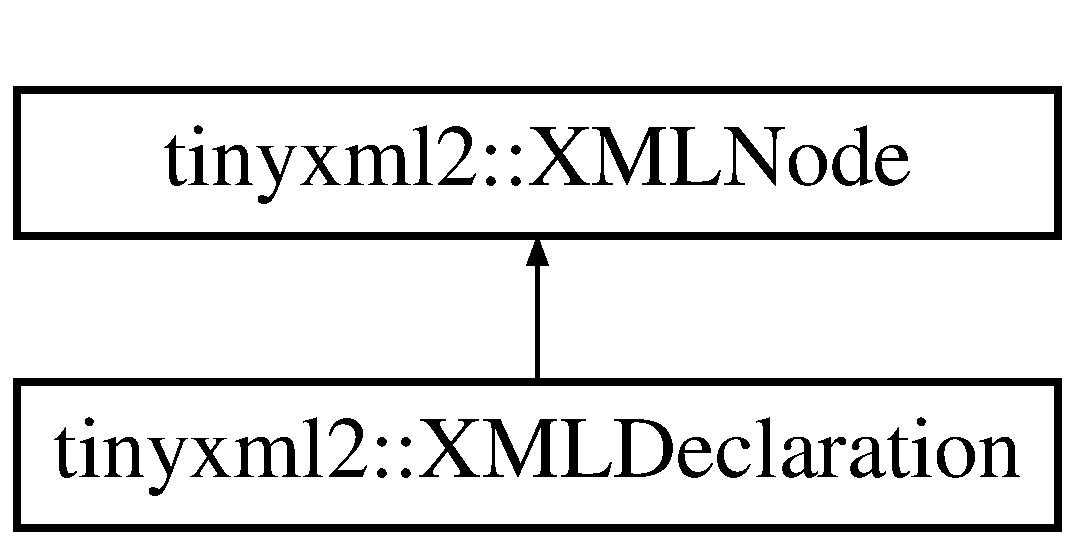
\includegraphics[height=2.000000cm]{classtinyxml2_1_1_x_m_l_declaration}
\end{center}
\end{figure}
\subsection*{Public Member Functions}
\begin{DoxyCompactItemize}
\item 
\hypertarget{classtinyxml2_1_1_x_m_l_declaration_a159d8ac45865215e88059ea1e5b52fc5}{virtual \hyperlink{classtinyxml2_1_1_x_m_l_declaration}{X\-M\-L\-Declaration} $\ast$ \hyperlink{classtinyxml2_1_1_x_m_l_declaration_a159d8ac45865215e88059ea1e5b52fc5}{To\-Declaration} ()}\label{classtinyxml2_1_1_x_m_l_declaration_a159d8ac45865215e88059ea1e5b52fc5}

\begin{DoxyCompactList}\small\item\em Safely cast to a Declaration, or null. \end{DoxyCompactList}\item 
\hypertarget{classtinyxml2_1_1_x_m_l_declaration_af724607a5fa810496fd6a21f5975a643}{virtual const \hyperlink{classtinyxml2_1_1_x_m_l_declaration}{X\-M\-L\-Declaration} $\ast$ {\bfseries To\-Declaration} () const }\label{classtinyxml2_1_1_x_m_l_declaration_af724607a5fa810496fd6a21f5975a643}

\item 
virtual bool \hyperlink{classtinyxml2_1_1_x_m_l_declaration_a953a7359cc312d15218eb5843a4ca108}{Accept} (\hyperlink{classtinyxml2_1_1_x_m_l_visitor}{X\-M\-L\-Visitor} $\ast$visitor) const 
\item 
\hypertarget{classtinyxml2_1_1_x_m_l_declaration_a19e33e0a9f9500f449261558c36f9a44}{char $\ast$ {\bfseries Parse\-Deep} (char $\ast$, \hyperlink{classtinyxml2_1_1_str_pair}{Str\-Pair} $\ast$end\-Tag)}\label{classtinyxml2_1_1_x_m_l_declaration_a19e33e0a9f9500f449261558c36f9a44}

\item 
virtual \hyperlink{classtinyxml2_1_1_x_m_l_node}{X\-M\-L\-Node} $\ast$ \hyperlink{classtinyxml2_1_1_x_m_l_declaration_a39458732ee6796cfc85dd35d3c488e0b}{Shallow\-Clone} (\hyperlink{classtinyxml2_1_1_x_m_l_document}{X\-M\-L\-Document} $\ast$document) const 
\item 
virtual bool \hyperlink{classtinyxml2_1_1_x_m_l_declaration_ace0d2d9bc1b63278bd5e984ebe0c7bd0}{Shallow\-Equal} (const \hyperlink{classtinyxml2_1_1_x_m_l_node}{X\-M\-L\-Node} $\ast$compare) const 
\end{DoxyCompactItemize}
\subsection*{Protected Member Functions}
\begin{DoxyCompactItemize}
\item 
\hypertarget{classtinyxml2_1_1_x_m_l_declaration_aef9586f2ce5df5feba74dde49a242b06}{{\bfseries X\-M\-L\-Declaration} (\hyperlink{classtinyxml2_1_1_x_m_l_document}{X\-M\-L\-Document} $\ast$doc)}\label{classtinyxml2_1_1_x_m_l_declaration_aef9586f2ce5df5feba74dde49a242b06}

\item 
\hypertarget{classtinyxml2_1_1_x_m_l_declaration_a5229cc0b31f034f93289af27ec3e2836}{{\bfseries X\-M\-L\-Declaration} (const \hyperlink{classtinyxml2_1_1_x_m_l_declaration}{X\-M\-L\-Declaration} \&)}\label{classtinyxml2_1_1_x_m_l_declaration_a5229cc0b31f034f93289af27ec3e2836}

\item 
\hypertarget{classtinyxml2_1_1_x_m_l_declaration_a79eb518c2c2b1b99a122a5d5a308b7ee}{\hyperlink{classtinyxml2_1_1_x_m_l_declaration}{X\-M\-L\-Declaration} \& {\bfseries operator=} (const \hyperlink{classtinyxml2_1_1_x_m_l_declaration}{X\-M\-L\-Declaration} \&)}\label{classtinyxml2_1_1_x_m_l_declaration_a79eb518c2c2b1b99a122a5d5a308b7ee}

\end{DoxyCompactItemize}
\subsection*{Friends}
\begin{DoxyCompactItemize}
\item 
\hypertarget{classtinyxml2_1_1_x_m_l_declaration_a4eee3bda60c60a30e4e8cd4ea91c4c6e}{class {\bfseries X\-M\-L\-Document}}\label{classtinyxml2_1_1_x_m_l_declaration_a4eee3bda60c60a30e4e8cd4ea91c4c6e}

\end{DoxyCompactItemize}
\subsection*{Additional Inherited Members}


\subsection{Detailed Description}
In correct X\-M\-L the declaration is the first entry in the file. \begin{DoxyVerb}    <?xml version="1.0" standalone="yes"?>
\end{DoxyVerb}


Tiny\-X\-M\-L-\/2 will happily read or write files without a declaration, however.

The text of the declaration isn't interpreted. It is parsed and written as a string. 

\subsection{Member Function Documentation}
\hypertarget{classtinyxml2_1_1_x_m_l_declaration_a953a7359cc312d15218eb5843a4ca108}{\index{tinyxml2\-::\-X\-M\-L\-Declaration@{tinyxml2\-::\-X\-M\-L\-Declaration}!Accept@{Accept}}
\index{Accept@{Accept}!tinyxml2::XMLDeclaration@{tinyxml2\-::\-X\-M\-L\-Declaration}}
\subsubsection[{Accept}]{\setlength{\rightskip}{0pt plus 5cm}bool tinyxml2\-::\-X\-M\-L\-Declaration\-::\-Accept (
\begin{DoxyParamCaption}
\item[{{\bf X\-M\-L\-Visitor} $\ast$}]{visitor}
\end{DoxyParamCaption}
) const\hspace{0.3cm}{\ttfamily [virtual]}}}\label{classtinyxml2_1_1_x_m_l_declaration_a953a7359cc312d15218eb5843a4ca108}
Accept a hierarchical visit of the nodes in the Tiny\-X\-M\-L-\/2 D\-O\-M. Every node in the X\-M\-L tree will be conditionally visited and the host will be called back via the \hyperlink{classtinyxml2_1_1_x_m_l_visitor}{X\-M\-L\-Visitor} interface.

This is essentially a S\-A\-X interface for Tiny\-X\-M\-L-\/2. (Note however it doesn't re-\/parse the X\-M\-L for the callbacks, so the performance of Tiny\-X\-M\-L-\/2 is unchanged by using this interface versus any other.)

The interface has been based on ideas from\-:


\begin{DoxyItemize}
\item \href{http://www.saxproject.org/}{\tt http\-://www.\-saxproject.\-org/}
\item \href{http://c2.com/cgi/wiki?HierarchicalVisitorPattern}{\tt http\-://c2.\-com/cgi/wiki?\-Hierarchical\-Visitor\-Pattern}
\end{DoxyItemize}

Which are both good references for \char`\"{}visiting\char`\"{}.

An example of using \hyperlink{classtinyxml2_1_1_x_m_l_declaration_a953a7359cc312d15218eb5843a4ca108}{Accept()}\-: \begin{DoxyVerb}XMLPrinter printer;
tinyxmlDoc.Accept( &printer );
const char* xmlcstr = printer.CStr();
\end{DoxyVerb}
 

Implements \hyperlink{classtinyxml2_1_1_x_m_l_node_a81e66df0a44c67a7af17f3b77a152785}{tinyxml2\-::\-X\-M\-L\-Node}.

\hypertarget{classtinyxml2_1_1_x_m_l_declaration_a39458732ee6796cfc85dd35d3c488e0b}{\index{tinyxml2\-::\-X\-M\-L\-Declaration@{tinyxml2\-::\-X\-M\-L\-Declaration}!Shallow\-Clone@{Shallow\-Clone}}
\index{Shallow\-Clone@{Shallow\-Clone}!tinyxml2::XMLDeclaration@{tinyxml2\-::\-X\-M\-L\-Declaration}}
\subsubsection[{Shallow\-Clone}]{\setlength{\rightskip}{0pt plus 5cm}{\bf X\-M\-L\-Node} $\ast$ tinyxml2\-::\-X\-M\-L\-Declaration\-::\-Shallow\-Clone (
\begin{DoxyParamCaption}
\item[{{\bf X\-M\-L\-Document} $\ast$}]{document}
\end{DoxyParamCaption}
) const\hspace{0.3cm}{\ttfamily [virtual]}}}\label{classtinyxml2_1_1_x_m_l_declaration_a39458732ee6796cfc85dd35d3c488e0b}
Make a copy of this node, but not its children. You may pass in a Document pointer that will be the owner of the new Node. If the 'document' is null, then the node returned will be allocated from the current Document. (this-\/$>$\hyperlink{classtinyxml2_1_1_x_m_l_node_af343d1ef0b45c0020e62d784d7e67a68}{Get\-Document()})

Note\-: if called on a \hyperlink{classtinyxml2_1_1_x_m_l_document}{X\-M\-L\-Document}, this will return null. 

Implements \hyperlink{classtinyxml2_1_1_x_m_l_node_a8402cbd3129d20e9e6024bbcc0531283}{tinyxml2\-::\-X\-M\-L\-Node}.

\hypertarget{classtinyxml2_1_1_x_m_l_declaration_ace0d2d9bc1b63278bd5e984ebe0c7bd0}{\index{tinyxml2\-::\-X\-M\-L\-Declaration@{tinyxml2\-::\-X\-M\-L\-Declaration}!Shallow\-Equal@{Shallow\-Equal}}
\index{Shallow\-Equal@{Shallow\-Equal}!tinyxml2::XMLDeclaration@{tinyxml2\-::\-X\-M\-L\-Declaration}}
\subsubsection[{Shallow\-Equal}]{\setlength{\rightskip}{0pt plus 5cm}bool tinyxml2\-::\-X\-M\-L\-Declaration\-::\-Shallow\-Equal (
\begin{DoxyParamCaption}
\item[{const {\bf X\-M\-L\-Node} $\ast$}]{compare}
\end{DoxyParamCaption}
) const\hspace{0.3cm}{\ttfamily [virtual]}}}\label{classtinyxml2_1_1_x_m_l_declaration_ace0d2d9bc1b63278bd5e984ebe0c7bd0}
Test if 2 nodes are the same, but don't test children. The 2 nodes do not need to be in the same Document.

Note\-: if called on a \hyperlink{classtinyxml2_1_1_x_m_l_document}{X\-M\-L\-Document}, this will return false. 

Implements \hyperlink{classtinyxml2_1_1_x_m_l_node_a7ce18b751c3ea09eac292dca264f9226}{tinyxml2\-::\-X\-M\-L\-Node}.



The documentation for this class was generated from the following files\-:\begin{DoxyCompactItemize}
\item 
tinyxml2.\-h\item 
tinyxml2.\-cpp\end{DoxyCompactItemize}

\hypertarget{classtinyxml2_1_1_x_m_l_document}{\section{tinyxml2\-:\-:X\-M\-L\-Document Class Reference}
\label{classtinyxml2_1_1_x_m_l_document}\index{tinyxml2\-::\-X\-M\-L\-Document@{tinyxml2\-::\-X\-M\-L\-Document}}
}


{\ttfamily \#include $<$tinyxml2.\-h$>$}

Inheritance diagram for tinyxml2\-:\-:X\-M\-L\-Document\-:\begin{figure}[H]
\begin{center}
\leavevmode
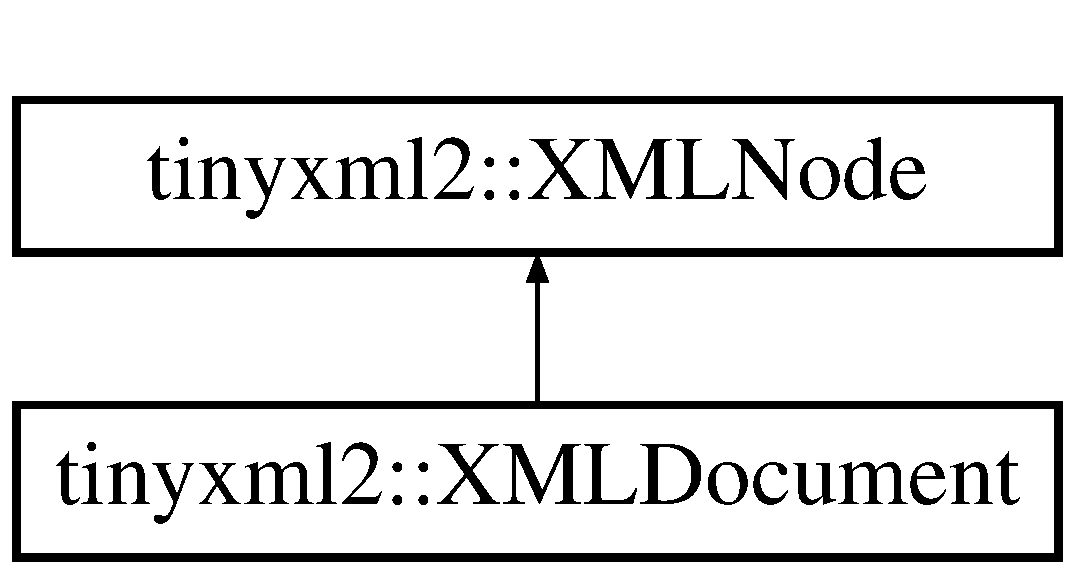
\includegraphics[height=2.000000cm]{classtinyxml2_1_1_x_m_l_document}
\end{center}
\end{figure}
\subsection*{Public Member Functions}
\begin{DoxyCompactItemize}
\item 
\hypertarget{classtinyxml2_1_1_x_m_l_document_af1574f76ebb619f25ef3f09eb2ba5188}{\hyperlink{classtinyxml2_1_1_x_m_l_document_af1574f76ebb619f25ef3f09eb2ba5188}{X\-M\-L\-Document} (bool process\-Entities=true, Whitespace=P\-R\-E\-S\-E\-R\-V\-E\-\_\-\-W\-H\-I\-T\-E\-S\-P\-A\-C\-E)}\label{classtinyxml2_1_1_x_m_l_document_af1574f76ebb619f25ef3f09eb2ba5188}

\begin{DoxyCompactList}\small\item\em constructor \end{DoxyCompactList}\item 
\hypertarget{classtinyxml2_1_1_x_m_l_document_a3e185f880882bd978367bb55937735ec}{virtual \hyperlink{classtinyxml2_1_1_x_m_l_document}{X\-M\-L\-Document} $\ast$ \hyperlink{classtinyxml2_1_1_x_m_l_document_a3e185f880882bd978367bb55937735ec}{To\-Document} ()}\label{classtinyxml2_1_1_x_m_l_document_a3e185f880882bd978367bb55937735ec}

\begin{DoxyCompactList}\small\item\em Safely cast to a Document, or null. \end{DoxyCompactList}\item 
\hypertarget{classtinyxml2_1_1_x_m_l_document_a15eb1a62afa18c66808031da647d1129}{virtual const \hyperlink{classtinyxml2_1_1_x_m_l_document}{X\-M\-L\-Document} $\ast$ {\bfseries To\-Document} () const }\label{classtinyxml2_1_1_x_m_l_document_a15eb1a62afa18c66808031da647d1129}

\item 
X\-M\-L\-Error \hyperlink{classtinyxml2_1_1_x_m_l_document_a1819bd34f540a7304c105a6232d25a1f}{Parse} (const char $\ast$xml, size\-\_\-t n\-Bytes=(size\-\_\-t)(-\/1))
\item 
X\-M\-L\-Error \hyperlink{classtinyxml2_1_1_x_m_l_document_a2ebd4647a8af5fc6831b294ac26a150a}{Load\-File} (const char $\ast$filename)
\item 
X\-M\-L\-Error \hyperlink{classtinyxml2_1_1_x_m_l_document_a5f1d330fad44c52f3d265338dd2a6dc2}{Load\-File} (F\-I\-L\-E $\ast$)
\item 
X\-M\-L\-Error \hyperlink{classtinyxml2_1_1_x_m_l_document_a73ac416b4a2aa0952e841220eb3da18f}{Save\-File} (const char $\ast$filename, bool compact=false)
\item 
X\-M\-L\-Error \hyperlink{classtinyxml2_1_1_x_m_l_document_a8b95779479a0035acc67b3a61dfe1b74}{Save\-File} (F\-I\-L\-E $\ast$fp, bool compact=false)
\item 
\hypertarget{classtinyxml2_1_1_x_m_l_document_adfcff7d0599cd520e9fcbb8891e1b678}{bool {\bfseries Process\-Entities} () const }\label{classtinyxml2_1_1_x_m_l_document_adfcff7d0599cd520e9fcbb8891e1b678}

\item 
\hypertarget{classtinyxml2_1_1_x_m_l_document_a94b3ea2f77c9ac831723984df5a02d01}{Whitespace {\bfseries Whitespace\-Mode} () const }\label{classtinyxml2_1_1_x_m_l_document_a94b3ea2f77c9ac831723984df5a02d01}

\item 
bool \hyperlink{classtinyxml2_1_1_x_m_l_document_a530649e9de7e5aa8df9c37f66197fcb6}{Has\-B\-O\-M} () const 
\item 
void \hyperlink{classtinyxml2_1_1_x_m_l_document_a14419b698f7c4b140df4e80f3f0c93b0}{Set\-B\-O\-M} (bool use\-B\-O\-M)
\item 
\hyperlink{classtinyxml2_1_1_x_m_l_element}{X\-M\-L\-Element} $\ast$ \hyperlink{classtinyxml2_1_1_x_m_l_document_ad2b70320d3c2a071c2f36928edff3e1c}{Root\-Element} ()
\item 
\hypertarget{classtinyxml2_1_1_x_m_l_document_a23a25b573d2adf3ee6075636c2a31c73}{const \hyperlink{classtinyxml2_1_1_x_m_l_element}{X\-M\-L\-Element} $\ast$ {\bfseries Root\-Element} () const }\label{classtinyxml2_1_1_x_m_l_document_a23a25b573d2adf3ee6075636c2a31c73}

\item 
void \hyperlink{classtinyxml2_1_1_x_m_l_document_a686ea28672c0e0c60383ec28148c1ac0}{Print} (\hyperlink{classtinyxml2_1_1_x_m_l_printer}{X\-M\-L\-Printer} $\ast$streamer=0) const 
\item 
virtual bool \hyperlink{classtinyxml2_1_1_x_m_l_document_aa08503d24898bf9992ae5e5fb8b0cf87}{Accept} (\hyperlink{classtinyxml2_1_1_x_m_l_visitor}{X\-M\-L\-Visitor} $\ast$visitor) const 
\item 
\hyperlink{classtinyxml2_1_1_x_m_l_element}{X\-M\-L\-Element} $\ast$ \hyperlink{classtinyxml2_1_1_x_m_l_document_a3c335a700a43d7c363a393142a23f234}{New\-Element} (const char $\ast$name)
\item 
\hyperlink{classtinyxml2_1_1_x_m_l_comment}{X\-M\-L\-Comment} $\ast$ \hyperlink{classtinyxml2_1_1_x_m_l_document_a386df0befd06aadb5e0cd21381aa955a}{New\-Comment} (const char $\ast$comment)
\item 
\hyperlink{classtinyxml2_1_1_x_m_l_text}{X\-M\-L\-Text} $\ast$ \hyperlink{classtinyxml2_1_1_x_m_l_document_acece5de77a0819f2341b08c1e1ed9987}{New\-Text} (const char $\ast$text)
\item 
\hyperlink{classtinyxml2_1_1_x_m_l_declaration}{X\-M\-L\-Declaration} $\ast$ \hyperlink{classtinyxml2_1_1_x_m_l_document_ae519030c0262fa2daff8993681990e16}{New\-Declaration} (const char $\ast$text=0)
\item 
\hyperlink{classtinyxml2_1_1_x_m_l_unknown}{X\-M\-L\-Unknown} $\ast$ \hyperlink{classtinyxml2_1_1_x_m_l_document_a4954f502c5fd7f49de54c3c0c99bb73d}{New\-Unknown} (const char $\ast$text)
\item 
void \hyperlink{classtinyxml2_1_1_x_m_l_document_ac1d6e2c7fcc1a660624ac4f68e96380d}{Delete\-Node} (\hyperlink{classtinyxml2_1_1_x_m_l_node}{X\-M\-L\-Node} $\ast$node)
\item 
\hypertarget{classtinyxml2_1_1_x_m_l_document_ae38d194e47336e4c96677ac77e2ac5d4}{void {\bfseries Set\-Error} (X\-M\-L\-Error error, const char $\ast$str1, const char $\ast$str2)}\label{classtinyxml2_1_1_x_m_l_document_ae38d194e47336e4c96677ac77e2ac5d4}

\item 
\hypertarget{classtinyxml2_1_1_x_m_l_document_abf0f9ac4c3aa5698a785937f71f7a69f}{bool \hyperlink{classtinyxml2_1_1_x_m_l_document_abf0f9ac4c3aa5698a785937f71f7a69f}{Error} () const }\label{classtinyxml2_1_1_x_m_l_document_abf0f9ac4c3aa5698a785937f71f7a69f}

\begin{DoxyCompactList}\small\item\em Return true if there was an error parsing the document. \end{DoxyCompactList}\item 
\hypertarget{classtinyxml2_1_1_x_m_l_document_a34903418c9e83f27945c2c533839e350}{X\-M\-L\-Error \hyperlink{classtinyxml2_1_1_x_m_l_document_a34903418c9e83f27945c2c533839e350}{Error\-I\-D} () const }\label{classtinyxml2_1_1_x_m_l_document_a34903418c9e83f27945c2c533839e350}

\begin{DoxyCompactList}\small\item\em Return the error\-I\-D. \end{DoxyCompactList}\item 
\hypertarget{classtinyxml2_1_1_x_m_l_document_a016ccebecee36fe92084b5dfee6cc072}{const char $\ast$ \hyperlink{classtinyxml2_1_1_x_m_l_document_a016ccebecee36fe92084b5dfee6cc072}{Get\-Error\-Str1} () const }\label{classtinyxml2_1_1_x_m_l_document_a016ccebecee36fe92084b5dfee6cc072}

\begin{DoxyCompactList}\small\item\em Return a possibly helpful diagnostic location or string. \end{DoxyCompactList}\item 
\hypertarget{classtinyxml2_1_1_x_m_l_document_a88f6b44bd019033bda28abd31fe257b2}{const char $\ast$ \hyperlink{classtinyxml2_1_1_x_m_l_document_a88f6b44bd019033bda28abd31fe257b2}{Get\-Error\-Str2} () const }\label{classtinyxml2_1_1_x_m_l_document_a88f6b44bd019033bda28abd31fe257b2}

\begin{DoxyCompactList}\small\item\em Return a possibly helpful secondary diagnostic location or string. \end{DoxyCompactList}\item 
\hypertarget{classtinyxml2_1_1_x_m_l_document_a7545cc9a9a67eee9307c001aa316a388}{void \hyperlink{classtinyxml2_1_1_x_m_l_document_a7545cc9a9a67eee9307c001aa316a388}{Print\-Error} () const }\label{classtinyxml2_1_1_x_m_l_document_a7545cc9a9a67eee9307c001aa316a388}

\begin{DoxyCompactList}\small\item\em If there is an error, print it to stdout. \end{DoxyCompactList}\item 
\hypertarget{classtinyxml2_1_1_x_m_l_document_a65656b0b2cbc822708eb351504178aaf}{void \hyperlink{classtinyxml2_1_1_x_m_l_document_a65656b0b2cbc822708eb351504178aaf}{Clear} ()}\label{classtinyxml2_1_1_x_m_l_document_a65656b0b2cbc822708eb351504178aaf}

\begin{DoxyCompactList}\small\item\em Clear the document, resetting it to the initial state. \end{DoxyCompactList}\item 
\hypertarget{classtinyxml2_1_1_x_m_l_document_a25827d1bec509ad566a107e5853ed040}{char $\ast$ {\bfseries Identify} (char $\ast$p, \hyperlink{classtinyxml2_1_1_x_m_l_node}{X\-M\-L\-Node} $\ast$$\ast$node)}\label{classtinyxml2_1_1_x_m_l_document_a25827d1bec509ad566a107e5853ed040}

\item 
virtual \hyperlink{classtinyxml2_1_1_x_m_l_node}{X\-M\-L\-Node} $\ast$ \hyperlink{classtinyxml2_1_1_x_m_l_document_a57c8511ed9f83aa3e20909a3db3f83d0}{Shallow\-Clone} (\hyperlink{classtinyxml2_1_1_x_m_l_document}{X\-M\-L\-Document} $\ast$) const 
\item 
virtual bool \hyperlink{classtinyxml2_1_1_x_m_l_document_a12eac66c6e45d074d5cc47319868cd66}{Shallow\-Equal} (const \hyperlink{classtinyxml2_1_1_x_m_l_node}{X\-M\-L\-Node} $\ast$) const 
\end{DoxyCompactItemize}
\subsection*{Friends}
\begin{DoxyCompactItemize}
\item 
\hypertarget{classtinyxml2_1_1_x_m_l_document_ac2fba9b6e452829dd892f7392c24e0eb}{class {\bfseries X\-M\-L\-Element}}\label{classtinyxml2_1_1_x_m_l_document_ac2fba9b6e452829dd892f7392c24e0eb}

\end{DoxyCompactItemize}
\subsection*{Additional Inherited Members}


\subsection{Detailed Description}
A Document binds together all the functionality. It can be saved, loaded, and printed to the screen. All Nodes are connected and allocated to a Document. If the Document is deleted, all its Nodes are also deleted. 

\subsection{Member Function Documentation}
\hypertarget{classtinyxml2_1_1_x_m_l_document_aa08503d24898bf9992ae5e5fb8b0cf87}{\index{tinyxml2\-::\-X\-M\-L\-Document@{tinyxml2\-::\-X\-M\-L\-Document}!Accept@{Accept}}
\index{Accept@{Accept}!tinyxml2::XMLDocument@{tinyxml2\-::\-X\-M\-L\-Document}}
\subsubsection[{Accept}]{\setlength{\rightskip}{0pt plus 5cm}bool tinyxml2\-::\-X\-M\-L\-Document\-::\-Accept (
\begin{DoxyParamCaption}
\item[{{\bf X\-M\-L\-Visitor} $\ast$}]{visitor}
\end{DoxyParamCaption}
) const\hspace{0.3cm}{\ttfamily [virtual]}}}\label{classtinyxml2_1_1_x_m_l_document_aa08503d24898bf9992ae5e5fb8b0cf87}
Accept a hierarchical visit of the nodes in the Tiny\-X\-M\-L-\/2 D\-O\-M. Every node in the X\-M\-L tree will be conditionally visited and the host will be called back via the \hyperlink{classtinyxml2_1_1_x_m_l_visitor}{X\-M\-L\-Visitor} interface.

This is essentially a S\-A\-X interface for Tiny\-X\-M\-L-\/2. (Note however it doesn't re-\/parse the X\-M\-L for the callbacks, so the performance of Tiny\-X\-M\-L-\/2 is unchanged by using this interface versus any other.)

The interface has been based on ideas from\-:


\begin{DoxyItemize}
\item \href{http://www.saxproject.org/}{\tt http\-://www.\-saxproject.\-org/}
\item \href{http://c2.com/cgi/wiki?HierarchicalVisitorPattern}{\tt http\-://c2.\-com/cgi/wiki?\-Hierarchical\-Visitor\-Pattern}
\end{DoxyItemize}

Which are both good references for \char`\"{}visiting\char`\"{}.

An example of using \hyperlink{classtinyxml2_1_1_x_m_l_document_aa08503d24898bf9992ae5e5fb8b0cf87}{Accept()}\-: \begin{DoxyVerb}XMLPrinter printer;
tinyxmlDoc.Accept( &printer );
const char* xmlcstr = printer.CStr();
\end{DoxyVerb}
 

Implements \hyperlink{classtinyxml2_1_1_x_m_l_node_a81e66df0a44c67a7af17f3b77a152785}{tinyxml2\-::\-X\-M\-L\-Node}.

\hypertarget{classtinyxml2_1_1_x_m_l_document_ac1d6e2c7fcc1a660624ac4f68e96380d}{\index{tinyxml2\-::\-X\-M\-L\-Document@{tinyxml2\-::\-X\-M\-L\-Document}!Delete\-Node@{Delete\-Node}}
\index{Delete\-Node@{Delete\-Node}!tinyxml2::XMLDocument@{tinyxml2\-::\-X\-M\-L\-Document}}
\subsubsection[{Delete\-Node}]{\setlength{\rightskip}{0pt plus 5cm}void tinyxml2\-::\-X\-M\-L\-Document\-::\-Delete\-Node (
\begin{DoxyParamCaption}
\item[{{\bf X\-M\-L\-Node} $\ast$}]{node}
\end{DoxyParamCaption}
)\hspace{0.3cm}{\ttfamily [inline]}}}\label{classtinyxml2_1_1_x_m_l_document_ac1d6e2c7fcc1a660624ac4f68e96380d}
Delete a node associated with this document. It will be unlinked from the D\-O\-M. \hypertarget{classtinyxml2_1_1_x_m_l_document_a530649e9de7e5aa8df9c37f66197fcb6}{\index{tinyxml2\-::\-X\-M\-L\-Document@{tinyxml2\-::\-X\-M\-L\-Document}!Has\-B\-O\-M@{Has\-B\-O\-M}}
\index{Has\-B\-O\-M@{Has\-B\-O\-M}!tinyxml2::XMLDocument@{tinyxml2\-::\-X\-M\-L\-Document}}
\subsubsection[{Has\-B\-O\-M}]{\setlength{\rightskip}{0pt plus 5cm}bool tinyxml2\-::\-X\-M\-L\-Document\-::\-Has\-B\-O\-M (
\begin{DoxyParamCaption}
{}
\end{DoxyParamCaption}
) const\hspace{0.3cm}{\ttfamily [inline]}}}\label{classtinyxml2_1_1_x_m_l_document_a530649e9de7e5aa8df9c37f66197fcb6}
Returns true if this document has a leading Byte Order Mark of U\-T\-F8. \hypertarget{classtinyxml2_1_1_x_m_l_document_a2ebd4647a8af5fc6831b294ac26a150a}{\index{tinyxml2\-::\-X\-M\-L\-Document@{tinyxml2\-::\-X\-M\-L\-Document}!Load\-File@{Load\-File}}
\index{Load\-File@{Load\-File}!tinyxml2::XMLDocument@{tinyxml2\-::\-X\-M\-L\-Document}}
\subsubsection[{Load\-File}]{\setlength{\rightskip}{0pt plus 5cm}X\-M\-L\-Error tinyxml2\-::\-X\-M\-L\-Document\-::\-Load\-File (
\begin{DoxyParamCaption}
\item[{const char $\ast$}]{filename}
\end{DoxyParamCaption}
)}}\label{classtinyxml2_1_1_x_m_l_document_a2ebd4647a8af5fc6831b294ac26a150a}
Load an X\-M\-L file from disk. Returns X\-M\-L\-\_\-\-N\-O\-\_\-\-E\-R\-R\-O\-R (0) on success, or an error\-I\-D. \hypertarget{classtinyxml2_1_1_x_m_l_document_a5f1d330fad44c52f3d265338dd2a6dc2}{\index{tinyxml2\-::\-X\-M\-L\-Document@{tinyxml2\-::\-X\-M\-L\-Document}!Load\-File@{Load\-File}}
\index{Load\-File@{Load\-File}!tinyxml2::XMLDocument@{tinyxml2\-::\-X\-M\-L\-Document}}
\subsubsection[{Load\-File}]{\setlength{\rightskip}{0pt plus 5cm}X\-M\-L\-Error tinyxml2\-::\-X\-M\-L\-Document\-::\-Load\-File (
\begin{DoxyParamCaption}
\item[{F\-I\-L\-E $\ast$}]{fp}
\end{DoxyParamCaption}
)}}\label{classtinyxml2_1_1_x_m_l_document_a5f1d330fad44c52f3d265338dd2a6dc2}
Load an X\-M\-L file from disk. You are responsible for providing and closing the F\-I\-L\-E$\ast$.

Returns X\-M\-L\-\_\-\-N\-O\-\_\-\-E\-R\-R\-O\-R (0) on success, or an error\-I\-D. \hypertarget{classtinyxml2_1_1_x_m_l_document_a386df0befd06aadb5e0cd21381aa955a}{\index{tinyxml2\-::\-X\-M\-L\-Document@{tinyxml2\-::\-X\-M\-L\-Document}!New\-Comment@{New\-Comment}}
\index{New\-Comment@{New\-Comment}!tinyxml2::XMLDocument@{tinyxml2\-::\-X\-M\-L\-Document}}
\subsubsection[{New\-Comment}]{\setlength{\rightskip}{0pt plus 5cm}{\bf X\-M\-L\-Comment} $\ast$ tinyxml2\-::\-X\-M\-L\-Document\-::\-New\-Comment (
\begin{DoxyParamCaption}
\item[{const char $\ast$}]{comment}
\end{DoxyParamCaption}
)}}\label{classtinyxml2_1_1_x_m_l_document_a386df0befd06aadb5e0cd21381aa955a}
Create a new Comment associated with this Document. The memory for the Comment is managed by the Document. \hypertarget{classtinyxml2_1_1_x_m_l_document_ae519030c0262fa2daff8993681990e16}{\index{tinyxml2\-::\-X\-M\-L\-Document@{tinyxml2\-::\-X\-M\-L\-Document}!New\-Declaration@{New\-Declaration}}
\index{New\-Declaration@{New\-Declaration}!tinyxml2::XMLDocument@{tinyxml2\-::\-X\-M\-L\-Document}}
\subsubsection[{New\-Declaration}]{\setlength{\rightskip}{0pt plus 5cm}{\bf X\-M\-L\-Declaration} $\ast$ tinyxml2\-::\-X\-M\-L\-Document\-::\-New\-Declaration (
\begin{DoxyParamCaption}
\item[{const char $\ast$}]{text = {\ttfamily 0}}
\end{DoxyParamCaption}
)}}\label{classtinyxml2_1_1_x_m_l_document_ae519030c0262fa2daff8993681990e16}
Create a new Declaration associated with this Document. The memory for the object is managed by the Document.

If the 'text' param is null, the standard declaration is used.\-: \begin{DoxyVerb}    <?xml version="1.0" encoding="UTF-8"?>
\end{DoxyVerb}
 \hypertarget{classtinyxml2_1_1_x_m_l_document_a3c335a700a43d7c363a393142a23f234}{\index{tinyxml2\-::\-X\-M\-L\-Document@{tinyxml2\-::\-X\-M\-L\-Document}!New\-Element@{New\-Element}}
\index{New\-Element@{New\-Element}!tinyxml2::XMLDocument@{tinyxml2\-::\-X\-M\-L\-Document}}
\subsubsection[{New\-Element}]{\setlength{\rightskip}{0pt plus 5cm}{\bf X\-M\-L\-Element} $\ast$ tinyxml2\-::\-X\-M\-L\-Document\-::\-New\-Element (
\begin{DoxyParamCaption}
\item[{const char $\ast$}]{name}
\end{DoxyParamCaption}
)}}\label{classtinyxml2_1_1_x_m_l_document_a3c335a700a43d7c363a393142a23f234}
Create a new Element associated with this Document. The memory for the Element is managed by the Document. \hypertarget{classtinyxml2_1_1_x_m_l_document_acece5de77a0819f2341b08c1e1ed9987}{\index{tinyxml2\-::\-X\-M\-L\-Document@{tinyxml2\-::\-X\-M\-L\-Document}!New\-Text@{New\-Text}}
\index{New\-Text@{New\-Text}!tinyxml2::XMLDocument@{tinyxml2\-::\-X\-M\-L\-Document}}
\subsubsection[{New\-Text}]{\setlength{\rightskip}{0pt plus 5cm}{\bf X\-M\-L\-Text} $\ast$ tinyxml2\-::\-X\-M\-L\-Document\-::\-New\-Text (
\begin{DoxyParamCaption}
\item[{const char $\ast$}]{text}
\end{DoxyParamCaption}
)}}\label{classtinyxml2_1_1_x_m_l_document_acece5de77a0819f2341b08c1e1ed9987}
Create a new Text associated with this Document. The memory for the Text is managed by the Document. \hypertarget{classtinyxml2_1_1_x_m_l_document_a4954f502c5fd7f49de54c3c0c99bb73d}{\index{tinyxml2\-::\-X\-M\-L\-Document@{tinyxml2\-::\-X\-M\-L\-Document}!New\-Unknown@{New\-Unknown}}
\index{New\-Unknown@{New\-Unknown}!tinyxml2::XMLDocument@{tinyxml2\-::\-X\-M\-L\-Document}}
\subsubsection[{New\-Unknown}]{\setlength{\rightskip}{0pt plus 5cm}{\bf X\-M\-L\-Unknown} $\ast$ tinyxml2\-::\-X\-M\-L\-Document\-::\-New\-Unknown (
\begin{DoxyParamCaption}
\item[{const char $\ast$}]{text}
\end{DoxyParamCaption}
)}}\label{classtinyxml2_1_1_x_m_l_document_a4954f502c5fd7f49de54c3c0c99bb73d}
Create a new Unknown associated with this Document. The memory for the object is managed by the Document. \hypertarget{classtinyxml2_1_1_x_m_l_document_a1819bd34f540a7304c105a6232d25a1f}{\index{tinyxml2\-::\-X\-M\-L\-Document@{tinyxml2\-::\-X\-M\-L\-Document}!Parse@{Parse}}
\index{Parse@{Parse}!tinyxml2::XMLDocument@{tinyxml2\-::\-X\-M\-L\-Document}}
\subsubsection[{Parse}]{\setlength{\rightskip}{0pt plus 5cm}X\-M\-L\-Error tinyxml2\-::\-X\-M\-L\-Document\-::\-Parse (
\begin{DoxyParamCaption}
\item[{const char $\ast$}]{xml, }
\item[{size\-\_\-t}]{n\-Bytes = {\ttfamily (size\-\_\-t)(-\/1)}}
\end{DoxyParamCaption}
)}}\label{classtinyxml2_1_1_x_m_l_document_a1819bd34f540a7304c105a6232d25a1f}
Parse an X\-M\-L file from a character string. Returns X\-M\-L\-\_\-\-N\-O\-\_\-\-E\-R\-R\-O\-R (0) on success, or an error\-I\-D.

You may optionally pass in the 'n\-Bytes', which is the number of bytes which will be parsed. If not specified, Tiny\-X\-M\-L-\/2 will assume 'xml' points to a null terminated string. \hypertarget{classtinyxml2_1_1_x_m_l_document_a686ea28672c0e0c60383ec28148c1ac0}{\index{tinyxml2\-::\-X\-M\-L\-Document@{tinyxml2\-::\-X\-M\-L\-Document}!Print@{Print}}
\index{Print@{Print}!tinyxml2::XMLDocument@{tinyxml2\-::\-X\-M\-L\-Document}}
\subsubsection[{Print}]{\setlength{\rightskip}{0pt plus 5cm}void tinyxml2\-::\-X\-M\-L\-Document\-::\-Print (
\begin{DoxyParamCaption}
\item[{{\bf X\-M\-L\-Printer} $\ast$}]{streamer = {\ttfamily 0}}
\end{DoxyParamCaption}
) const}}\label{classtinyxml2_1_1_x_m_l_document_a686ea28672c0e0c60383ec28148c1ac0}
Print the Document. If the Printer is not provided, it will print to stdout. If you provide Printer, this can print to a file\-: \begin{DoxyVerb}XMLPrinter printer( fp );
doc.Print( &printer );
\end{DoxyVerb}


Or you can use a printer to print to memory\-: \begin{DoxyVerb}XMLPrinter printer;
doc.Print( &printer );
// printer.CStr() has a const char* to the XML
\end{DoxyVerb}
 \hypertarget{classtinyxml2_1_1_x_m_l_document_ad2b70320d3c2a071c2f36928edff3e1c}{\index{tinyxml2\-::\-X\-M\-L\-Document@{tinyxml2\-::\-X\-M\-L\-Document}!Root\-Element@{Root\-Element}}
\index{Root\-Element@{Root\-Element}!tinyxml2::XMLDocument@{tinyxml2\-::\-X\-M\-L\-Document}}
\subsubsection[{Root\-Element}]{\setlength{\rightskip}{0pt plus 5cm}{\bf X\-M\-L\-Element}$\ast$ tinyxml2\-::\-X\-M\-L\-Document\-::\-Root\-Element (
\begin{DoxyParamCaption}
{}
\end{DoxyParamCaption}
)\hspace{0.3cm}{\ttfamily [inline]}}}\label{classtinyxml2_1_1_x_m_l_document_ad2b70320d3c2a071c2f36928edff3e1c}
Return the root element of D\-O\-M. Equivalent to \hyperlink{classtinyxml2_1_1_x_m_l_node_a20f48e99b03e9c17487944f229bee130}{First\-Child\-Element()}. To get the first node, use First\-Child(). \hypertarget{classtinyxml2_1_1_x_m_l_document_a73ac416b4a2aa0952e841220eb3da18f}{\index{tinyxml2\-::\-X\-M\-L\-Document@{tinyxml2\-::\-X\-M\-L\-Document}!Save\-File@{Save\-File}}
\index{Save\-File@{Save\-File}!tinyxml2::XMLDocument@{tinyxml2\-::\-X\-M\-L\-Document}}
\subsubsection[{Save\-File}]{\setlength{\rightskip}{0pt plus 5cm}X\-M\-L\-Error tinyxml2\-::\-X\-M\-L\-Document\-::\-Save\-File (
\begin{DoxyParamCaption}
\item[{const char $\ast$}]{filename, }
\item[{bool}]{compact = {\ttfamily false}}
\end{DoxyParamCaption}
)}}\label{classtinyxml2_1_1_x_m_l_document_a73ac416b4a2aa0952e841220eb3da18f}
Save the X\-M\-L file to disk. Returns X\-M\-L\-\_\-\-N\-O\-\_\-\-E\-R\-R\-O\-R (0) on success, or an error\-I\-D. \hypertarget{classtinyxml2_1_1_x_m_l_document_a8b95779479a0035acc67b3a61dfe1b74}{\index{tinyxml2\-::\-X\-M\-L\-Document@{tinyxml2\-::\-X\-M\-L\-Document}!Save\-File@{Save\-File}}
\index{Save\-File@{Save\-File}!tinyxml2::XMLDocument@{tinyxml2\-::\-X\-M\-L\-Document}}
\subsubsection[{Save\-File}]{\setlength{\rightskip}{0pt plus 5cm}X\-M\-L\-Error tinyxml2\-::\-X\-M\-L\-Document\-::\-Save\-File (
\begin{DoxyParamCaption}
\item[{F\-I\-L\-E $\ast$}]{fp, }
\item[{bool}]{compact = {\ttfamily false}}
\end{DoxyParamCaption}
)}}\label{classtinyxml2_1_1_x_m_l_document_a8b95779479a0035acc67b3a61dfe1b74}
Save the X\-M\-L file to disk. You are responsible for providing and closing the F\-I\-L\-E$\ast$.

Returns X\-M\-L\-\_\-\-N\-O\-\_\-\-E\-R\-R\-O\-R (0) on success, or an error\-I\-D. \hypertarget{classtinyxml2_1_1_x_m_l_document_a14419b698f7c4b140df4e80f3f0c93b0}{\index{tinyxml2\-::\-X\-M\-L\-Document@{tinyxml2\-::\-X\-M\-L\-Document}!Set\-B\-O\-M@{Set\-B\-O\-M}}
\index{Set\-B\-O\-M@{Set\-B\-O\-M}!tinyxml2::XMLDocument@{tinyxml2\-::\-X\-M\-L\-Document}}
\subsubsection[{Set\-B\-O\-M}]{\setlength{\rightskip}{0pt plus 5cm}void tinyxml2\-::\-X\-M\-L\-Document\-::\-Set\-B\-O\-M (
\begin{DoxyParamCaption}
\item[{bool}]{use\-B\-O\-M}
\end{DoxyParamCaption}
)\hspace{0.3cm}{\ttfamily [inline]}}}\label{classtinyxml2_1_1_x_m_l_document_a14419b698f7c4b140df4e80f3f0c93b0}
Sets whether to write the B\-O\-M when writing the file. \hypertarget{classtinyxml2_1_1_x_m_l_document_a57c8511ed9f83aa3e20909a3db3f83d0}{\index{tinyxml2\-::\-X\-M\-L\-Document@{tinyxml2\-::\-X\-M\-L\-Document}!Shallow\-Clone@{Shallow\-Clone}}
\index{Shallow\-Clone@{Shallow\-Clone}!tinyxml2::XMLDocument@{tinyxml2\-::\-X\-M\-L\-Document}}
\subsubsection[{Shallow\-Clone}]{\setlength{\rightskip}{0pt plus 5cm}virtual {\bf X\-M\-L\-Node}$\ast$ tinyxml2\-::\-X\-M\-L\-Document\-::\-Shallow\-Clone (
\begin{DoxyParamCaption}
\item[{{\bf X\-M\-L\-Document} $\ast$}]{document}
\end{DoxyParamCaption}
) const\hspace{0.3cm}{\ttfamily [inline]}, {\ttfamily [virtual]}}}\label{classtinyxml2_1_1_x_m_l_document_a57c8511ed9f83aa3e20909a3db3f83d0}
Make a copy of this node, but not its children. You may pass in a Document pointer that will be the owner of the new Node. If the 'document' is null, then the node returned will be allocated from the current Document. (this-\/$>$\hyperlink{classtinyxml2_1_1_x_m_l_node_af343d1ef0b45c0020e62d784d7e67a68}{Get\-Document()})

Note\-: if called on a \hyperlink{classtinyxml2_1_1_x_m_l_document}{X\-M\-L\-Document}, this will return null. 

Implements \hyperlink{classtinyxml2_1_1_x_m_l_node_a8402cbd3129d20e9e6024bbcc0531283}{tinyxml2\-::\-X\-M\-L\-Node}.

\hypertarget{classtinyxml2_1_1_x_m_l_document_a12eac66c6e45d074d5cc47319868cd66}{\index{tinyxml2\-::\-X\-M\-L\-Document@{tinyxml2\-::\-X\-M\-L\-Document}!Shallow\-Equal@{Shallow\-Equal}}
\index{Shallow\-Equal@{Shallow\-Equal}!tinyxml2::XMLDocument@{tinyxml2\-::\-X\-M\-L\-Document}}
\subsubsection[{Shallow\-Equal}]{\setlength{\rightskip}{0pt plus 5cm}virtual bool tinyxml2\-::\-X\-M\-L\-Document\-::\-Shallow\-Equal (
\begin{DoxyParamCaption}
\item[{const {\bf X\-M\-L\-Node} $\ast$}]{compare}
\end{DoxyParamCaption}
) const\hspace{0.3cm}{\ttfamily [inline]}, {\ttfamily [virtual]}}}\label{classtinyxml2_1_1_x_m_l_document_a12eac66c6e45d074d5cc47319868cd66}
Test if 2 nodes are the same, but don't test children. The 2 nodes do not need to be in the same Document.

Note\-: if called on a \hyperlink{classtinyxml2_1_1_x_m_l_document}{X\-M\-L\-Document}, this will return false. 

Implements \hyperlink{classtinyxml2_1_1_x_m_l_node_a7ce18b751c3ea09eac292dca264f9226}{tinyxml2\-::\-X\-M\-L\-Node}.



The documentation for this class was generated from the following files\-:\begin{DoxyCompactItemize}
\item 
tinyxml2.\-h\item 
tinyxml2.\-cpp\end{DoxyCompactItemize}

\hypertarget{classtinyxml2_1_1_x_m_l_element}{\section{tinyxml2\-:\-:X\-M\-L\-Element Class Reference}
\label{classtinyxml2_1_1_x_m_l_element}\index{tinyxml2\-::\-X\-M\-L\-Element@{tinyxml2\-::\-X\-M\-L\-Element}}
}


{\ttfamily \#include $<$tinyxml2.\-h$>$}

Inheritance diagram for tinyxml2\-:\-:X\-M\-L\-Element\-:\begin{figure}[H]
\begin{center}
\leavevmode
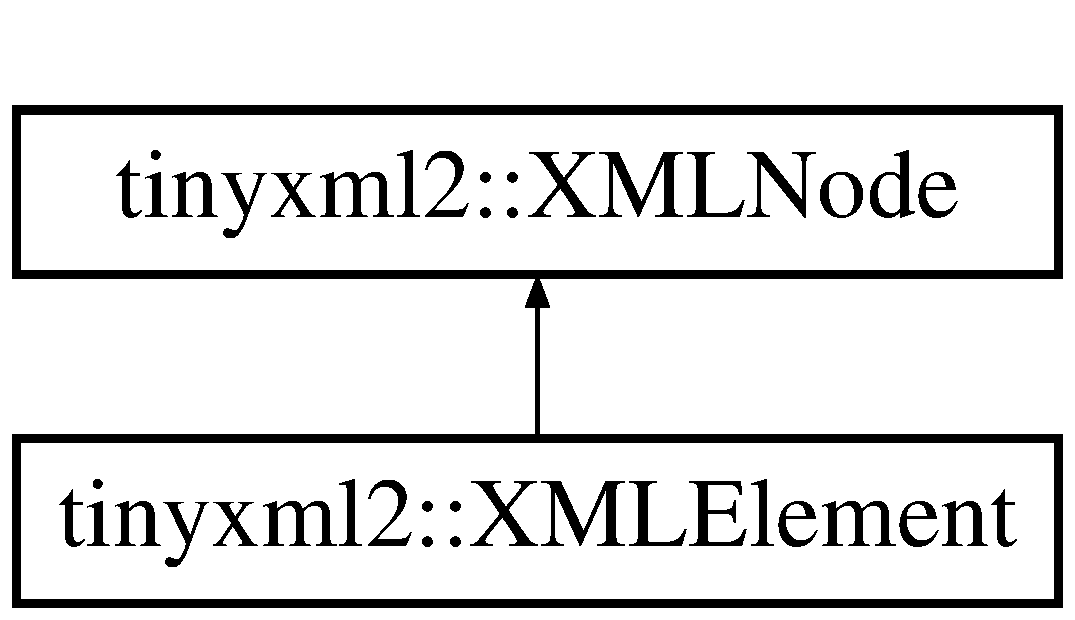
\includegraphics[height=2.000000cm]{classtinyxml2_1_1_x_m_l_element}
\end{center}
\end{figure}
\subsection*{Public Types}
\begin{DoxyCompactItemize}
\item 
enum \{ {\bfseries O\-P\-E\-N}, 
{\bfseries C\-L\-O\-S\-E\-D}, 
{\bfseries C\-L\-O\-S\-I\-N\-G}
 \}
\end{DoxyCompactItemize}
\subsection*{Public Member Functions}
\begin{DoxyCompactItemize}
\item 
\hypertarget{classtinyxml2_1_1_x_m_l_element_a8bff355472bce2c60d4b50a212bf7f5f}{const char $\ast$ \hyperlink{classtinyxml2_1_1_x_m_l_element_a8bff355472bce2c60d4b50a212bf7f5f}{Name} () const }\label{classtinyxml2_1_1_x_m_l_element_a8bff355472bce2c60d4b50a212bf7f5f}

\begin{DoxyCompactList}\small\item\em Get the name of an element (which is the \hyperlink{classtinyxml2_1_1_x_m_l_node_a7682be117e3b2b4ebfd517c1acaaadbf}{Value()} of the node.) \end{DoxyCompactList}\item 
\hypertarget{classtinyxml2_1_1_x_m_l_element_a97712009a530d8cb8a63bf705f02b4f1}{void \hyperlink{classtinyxml2_1_1_x_m_l_element_a97712009a530d8cb8a63bf705f02b4f1}{Set\-Name} (const char $\ast$str, bool static\-Mem=false)}\label{classtinyxml2_1_1_x_m_l_element_a97712009a530d8cb8a63bf705f02b4f1}

\begin{DoxyCompactList}\small\item\em Set the name of the element. \end{DoxyCompactList}\item 
\hypertarget{classtinyxml2_1_1_x_m_l_element_ad9ff5c2dbc15df36cf664ce1b0ea0a5d}{virtual \hyperlink{classtinyxml2_1_1_x_m_l_element}{X\-M\-L\-Element} $\ast$ \hyperlink{classtinyxml2_1_1_x_m_l_element_ad9ff5c2dbc15df36cf664ce1b0ea0a5d}{To\-Element} ()}\label{classtinyxml2_1_1_x_m_l_element_ad9ff5c2dbc15df36cf664ce1b0ea0a5d}

\begin{DoxyCompactList}\small\item\em Safely cast to an Element, or null. \end{DoxyCompactList}\item 
\hypertarget{classtinyxml2_1_1_x_m_l_element_a55acab615353ddabab48271f95816b0d}{virtual const \hyperlink{classtinyxml2_1_1_x_m_l_element}{X\-M\-L\-Element} $\ast$ {\bfseries To\-Element} () const }\label{classtinyxml2_1_1_x_m_l_element_a55acab615353ddabab48271f95816b0d}

\item 
virtual bool \hyperlink{classtinyxml2_1_1_x_m_l_element_a36d65438991a1e85096caf39ad13a099}{Accept} (\hyperlink{classtinyxml2_1_1_x_m_l_visitor}{X\-M\-L\-Visitor} $\ast$visitor) const 
\item 
const char $\ast$ \hyperlink{classtinyxml2_1_1_x_m_l_element_a7bdebdf1888074087237f3dd03912740}{Attribute} (const char $\ast$name, const char $\ast$value=0) const 
\item 
int \hyperlink{classtinyxml2_1_1_x_m_l_element_af86f05771c11a73a2896b662bb589ef5}{Int\-Attribute} (const char $\ast$name) const 
\item 
\hypertarget{classtinyxml2_1_1_x_m_l_element_aa5a41367b5118acec42a87f5f94cec2d}{unsigned \hyperlink{classtinyxml2_1_1_x_m_l_element_aa5a41367b5118acec42a87f5f94cec2d}{Unsigned\-Attribute} (const char $\ast$name) const }\label{classtinyxml2_1_1_x_m_l_element_aa5a41367b5118acec42a87f5f94cec2d}

\begin{DoxyCompactList}\small\item\em See \hyperlink{classtinyxml2_1_1_x_m_l_element_af86f05771c11a73a2896b662bb589ef5}{Int\-Attribute()} \end{DoxyCompactList}\item 
\hypertarget{classtinyxml2_1_1_x_m_l_element_a34811e4d1881e4ecc95c49f0f3799115}{bool \hyperlink{classtinyxml2_1_1_x_m_l_element_a34811e4d1881e4ecc95c49f0f3799115}{Bool\-Attribute} (const char $\ast$name) const }\label{classtinyxml2_1_1_x_m_l_element_a34811e4d1881e4ecc95c49f0f3799115}

\begin{DoxyCompactList}\small\item\em See \hyperlink{classtinyxml2_1_1_x_m_l_element_af86f05771c11a73a2896b662bb589ef5}{Int\-Attribute()} \end{DoxyCompactList}\item 
\hypertarget{classtinyxml2_1_1_x_m_l_element_a536922a5cae9c9769a3dc1b7a8ff0d44}{double \hyperlink{classtinyxml2_1_1_x_m_l_element_a536922a5cae9c9769a3dc1b7a8ff0d44}{Double\-Attribute} (const char $\ast$name) const }\label{classtinyxml2_1_1_x_m_l_element_a536922a5cae9c9769a3dc1b7a8ff0d44}

\begin{DoxyCompactList}\small\item\em See \hyperlink{classtinyxml2_1_1_x_m_l_element_af86f05771c11a73a2896b662bb589ef5}{Int\-Attribute()} \end{DoxyCompactList}\item 
\hypertarget{classtinyxml2_1_1_x_m_l_element_a33b69f123f995aff966d2e351bc51b1f}{float \hyperlink{classtinyxml2_1_1_x_m_l_element_a33b69f123f995aff966d2e351bc51b1f}{Float\-Attribute} (const char $\ast$name) const }\label{classtinyxml2_1_1_x_m_l_element_a33b69f123f995aff966d2e351bc51b1f}

\begin{DoxyCompactList}\small\item\em See \hyperlink{classtinyxml2_1_1_x_m_l_element_af86f05771c11a73a2896b662bb589ef5}{Int\-Attribute()} \end{DoxyCompactList}\item 
X\-M\-L\-Error \hyperlink{classtinyxml2_1_1_x_m_l_element_a8b92c729346aa8ea9acd59ed3e9f2378}{Query\-Int\-Attribute} (const char $\ast$name, int $\ast$value) const 
\item 
\hypertarget{classtinyxml2_1_1_x_m_l_element_aa3d8d1b9311da8fc249b4352749aaa84}{X\-M\-L\-Error \hyperlink{classtinyxml2_1_1_x_m_l_element_aa3d8d1b9311da8fc249b4352749aaa84}{Query\-Unsigned\-Attribute} (const char $\ast$name, unsigned int $\ast$value) const }\label{classtinyxml2_1_1_x_m_l_element_aa3d8d1b9311da8fc249b4352749aaa84}

\begin{DoxyCompactList}\small\item\em See \hyperlink{classtinyxml2_1_1_x_m_l_element_a8b92c729346aa8ea9acd59ed3e9f2378}{Query\-Int\-Attribute()} \end{DoxyCompactList}\item 
\hypertarget{classtinyxml2_1_1_x_m_l_element_a2a58ee941c3cda23772c887a8f8b534e}{X\-M\-L\-Error \hyperlink{classtinyxml2_1_1_x_m_l_element_a2a58ee941c3cda23772c887a8f8b534e}{Query\-Bool\-Attribute} (const char $\ast$name, bool $\ast$value) const }\label{classtinyxml2_1_1_x_m_l_element_a2a58ee941c3cda23772c887a8f8b534e}

\begin{DoxyCompactList}\small\item\em See \hyperlink{classtinyxml2_1_1_x_m_l_element_a8b92c729346aa8ea9acd59ed3e9f2378}{Query\-Int\-Attribute()} \end{DoxyCompactList}\item 
\hypertarget{classtinyxml2_1_1_x_m_l_element_a1ffeed461d3e4020b39652cd6d3cd773}{X\-M\-L\-Error \hyperlink{classtinyxml2_1_1_x_m_l_element_a1ffeed461d3e4020b39652cd6d3cd773}{Query\-Double\-Attribute} (const char $\ast$name, double $\ast$value) const }\label{classtinyxml2_1_1_x_m_l_element_a1ffeed461d3e4020b39652cd6d3cd773}

\begin{DoxyCompactList}\small\item\em See \hyperlink{classtinyxml2_1_1_x_m_l_element_a8b92c729346aa8ea9acd59ed3e9f2378}{Query\-Int\-Attribute()} \end{DoxyCompactList}\item 
\hypertarget{classtinyxml2_1_1_x_m_l_element_a3f154e0b4b6903249ff9f758921758e5}{X\-M\-L\-Error \hyperlink{classtinyxml2_1_1_x_m_l_element_a3f154e0b4b6903249ff9f758921758e5}{Query\-Float\-Attribute} (const char $\ast$name, float $\ast$value) const }\label{classtinyxml2_1_1_x_m_l_element_a3f154e0b4b6903249ff9f758921758e5}

\begin{DoxyCompactList}\small\item\em See \hyperlink{classtinyxml2_1_1_x_m_l_element_a8b92c729346aa8ea9acd59ed3e9f2378}{Query\-Int\-Attribute()} \end{DoxyCompactList}\item 
int \hyperlink{classtinyxml2_1_1_x_m_l_element_aa471a199af9f137ef371f5db1ed1016b}{Query\-Attribute} (const char $\ast$name, int $\ast$value) const 
\item 
\hypertarget{classtinyxml2_1_1_x_m_l_element_a60d18656aa70adb257eab18913aa4330}{int {\bfseries Query\-Attribute} (const char $\ast$name, unsigned int $\ast$value) const }\label{classtinyxml2_1_1_x_m_l_element_a60d18656aa70adb257eab18913aa4330}

\item 
\hypertarget{classtinyxml2_1_1_x_m_l_element_a23fa8bac4250249c476c6bfdb6cb9b9c}{int {\bfseries Query\-Attribute} (const char $\ast$name, bool $\ast$value) const }\label{classtinyxml2_1_1_x_m_l_element_a23fa8bac4250249c476c6bfdb6cb9b9c}

\item 
\hypertarget{classtinyxml2_1_1_x_m_l_element_a64aadcbf27423410e2896baf240f63f9}{int {\bfseries Query\-Attribute} (const char $\ast$name, double $\ast$value) const }\label{classtinyxml2_1_1_x_m_l_element_a64aadcbf27423410e2896baf240f63f9}

\item 
\hypertarget{classtinyxml2_1_1_x_m_l_element_afd553774be0e7760d73003058efa8df9}{int {\bfseries Query\-Attribute} (const char $\ast$name, float $\ast$value) const }\label{classtinyxml2_1_1_x_m_l_element_afd553774be0e7760d73003058efa8df9}

\item 
\hypertarget{classtinyxml2_1_1_x_m_l_element_a11943abf2d0831548c3790dd5d9f119c}{void \hyperlink{classtinyxml2_1_1_x_m_l_element_a11943abf2d0831548c3790dd5d9f119c}{Set\-Attribute} (const char $\ast$name, const char $\ast$value)}\label{classtinyxml2_1_1_x_m_l_element_a11943abf2d0831548c3790dd5d9f119c}

\begin{DoxyCompactList}\small\item\em Sets the named attribute to value. \end{DoxyCompactList}\item 
\hypertarget{classtinyxml2_1_1_x_m_l_element_aae6568c64c7f1cc88be8461ba41a79cf}{void \hyperlink{classtinyxml2_1_1_x_m_l_element_aae6568c64c7f1cc88be8461ba41a79cf}{Set\-Attribute} (const char $\ast$name, int value)}\label{classtinyxml2_1_1_x_m_l_element_aae6568c64c7f1cc88be8461ba41a79cf}

\begin{DoxyCompactList}\small\item\em Sets the named attribute to value. \end{DoxyCompactList}\item 
\hypertarget{classtinyxml2_1_1_x_m_l_element_ae143997e90064ba82326b29a9930ea8f}{void \hyperlink{classtinyxml2_1_1_x_m_l_element_ae143997e90064ba82326b29a9930ea8f}{Set\-Attribute} (const char $\ast$name, unsigned value)}\label{classtinyxml2_1_1_x_m_l_element_ae143997e90064ba82326b29a9930ea8f}

\begin{DoxyCompactList}\small\item\em Sets the named attribute to value. \end{DoxyCompactList}\item 
\hypertarget{classtinyxml2_1_1_x_m_l_element_aa848b696e6a75e4e545c6da9893b11e1}{void \hyperlink{classtinyxml2_1_1_x_m_l_element_aa848b696e6a75e4e545c6da9893b11e1}{Set\-Attribute} (const char $\ast$name, bool value)}\label{classtinyxml2_1_1_x_m_l_element_aa848b696e6a75e4e545c6da9893b11e1}

\begin{DoxyCompactList}\small\item\em Sets the named attribute to value. \end{DoxyCompactList}\item 
\hypertarget{classtinyxml2_1_1_x_m_l_element_a233397ee81e70eb5d4b814c5f8698533}{void \hyperlink{classtinyxml2_1_1_x_m_l_element_a233397ee81e70eb5d4b814c5f8698533}{Set\-Attribute} (const char $\ast$name, double value)}\label{classtinyxml2_1_1_x_m_l_element_a233397ee81e70eb5d4b814c5f8698533}

\begin{DoxyCompactList}\small\item\em Sets the named attribute to value. \end{DoxyCompactList}\item 
void \hyperlink{classtinyxml2_1_1_x_m_l_element_aebd45aa7118964c30b32fe12e944628a}{Delete\-Attribute} (const char $\ast$name)
\item 
\hypertarget{classtinyxml2_1_1_x_m_l_element_a67593e63558ffda0386699c3e4cc0b2c}{const \hyperlink{classtinyxml2_1_1_x_m_l_attribute}{X\-M\-L\-Attribute} $\ast$ \hyperlink{classtinyxml2_1_1_x_m_l_element_a67593e63558ffda0386699c3e4cc0b2c}{First\-Attribute} () const }\label{classtinyxml2_1_1_x_m_l_element_a67593e63558ffda0386699c3e4cc0b2c}

\begin{DoxyCompactList}\small\item\em Return the first attribute in the list. \end{DoxyCompactList}\item 
\hypertarget{classtinyxml2_1_1_x_m_l_element_aaf46b0799ea419e5d070ac9a357de48f}{const \hyperlink{classtinyxml2_1_1_x_m_l_attribute}{X\-M\-L\-Attribute} $\ast$ \hyperlink{classtinyxml2_1_1_x_m_l_element_aaf46b0799ea419e5d070ac9a357de48f}{Find\-Attribute} (const char $\ast$name) const }\label{classtinyxml2_1_1_x_m_l_element_aaf46b0799ea419e5d070ac9a357de48f}

\begin{DoxyCompactList}\small\item\em Query a specific attribute in the list. \end{DoxyCompactList}\item 
const char $\ast$ \hyperlink{classtinyxml2_1_1_x_m_l_element_a56cc727044dad002b978256754d43a4b}{Get\-Text} () const 
\item 
X\-M\-L\-Error \hyperlink{classtinyxml2_1_1_x_m_l_element_a71327c9a9d8840562bd204f46d0a7189}{Query\-Int\-Text} (int $\ast$ival) const 
\item 
\hypertarget{classtinyxml2_1_1_x_m_l_element_a2192091dec0c06be8b14f4e912c01758}{X\-M\-L\-Error \hyperlink{classtinyxml2_1_1_x_m_l_element_a2192091dec0c06be8b14f4e912c01758}{Query\-Unsigned\-Text} (unsigned $\ast$uval) const }\label{classtinyxml2_1_1_x_m_l_element_a2192091dec0c06be8b14f4e912c01758}

\begin{DoxyCompactList}\small\item\em See \hyperlink{classtinyxml2_1_1_x_m_l_element_a71327c9a9d8840562bd204f46d0a7189}{Query\-Int\-Text()} \end{DoxyCompactList}\item 
\hypertarget{classtinyxml2_1_1_x_m_l_element_afeb060672fa934163fc573e692b7fe38}{X\-M\-L\-Error \hyperlink{classtinyxml2_1_1_x_m_l_element_afeb060672fa934163fc573e692b7fe38}{Query\-Bool\-Text} (bool $\ast$bval) const }\label{classtinyxml2_1_1_x_m_l_element_afeb060672fa934163fc573e692b7fe38}

\begin{DoxyCompactList}\small\item\em See \hyperlink{classtinyxml2_1_1_x_m_l_element_a71327c9a9d8840562bd204f46d0a7189}{Query\-Int\-Text()} \end{DoxyCompactList}\item 
\hypertarget{classtinyxml2_1_1_x_m_l_element_aad931c42548907dbea416f7365d78b57}{X\-M\-L\-Error \hyperlink{classtinyxml2_1_1_x_m_l_element_aad931c42548907dbea416f7365d78b57}{Query\-Double\-Text} (double $\ast$dval) const }\label{classtinyxml2_1_1_x_m_l_element_aad931c42548907dbea416f7365d78b57}

\begin{DoxyCompactList}\small\item\em See \hyperlink{classtinyxml2_1_1_x_m_l_element_a71327c9a9d8840562bd204f46d0a7189}{Query\-Int\-Text()} \end{DoxyCompactList}\item 
\hypertarget{classtinyxml2_1_1_x_m_l_element_a11fa26e1dbca88e973964c1d9b597658}{X\-M\-L\-Error \hyperlink{classtinyxml2_1_1_x_m_l_element_a11fa26e1dbca88e973964c1d9b597658}{Query\-Float\-Text} (float $\ast$fval) const }\label{classtinyxml2_1_1_x_m_l_element_a11fa26e1dbca88e973964c1d9b597658}

\begin{DoxyCompactList}\small\item\em See \hyperlink{classtinyxml2_1_1_x_m_l_element_a71327c9a9d8840562bd204f46d0a7189}{Query\-Int\-Text()} \end{DoxyCompactList}\item 
\hypertarget{classtinyxml2_1_1_x_m_l_element_a2e3d9f938307a05963d7c4b8cd55754e}{int {\bfseries Closing\-Type} () const }\label{classtinyxml2_1_1_x_m_l_element_a2e3d9f938307a05963d7c4b8cd55754e}

\item 
\hypertarget{classtinyxml2_1_1_x_m_l_element_aaafdd2a5618abe80a2c1839ad3ccd492}{char $\ast$ {\bfseries Parse\-Deep} (char $\ast$p, \hyperlink{classtinyxml2_1_1_str_pair}{Str\-Pair} $\ast$end\-Tag)}\label{classtinyxml2_1_1_x_m_l_element_aaafdd2a5618abe80a2c1839ad3ccd492}

\item 
virtual \hyperlink{classtinyxml2_1_1_x_m_l_node}{X\-M\-L\-Node} $\ast$ \hyperlink{classtinyxml2_1_1_x_m_l_element_a85d85e32c18863fff1eeed53ae1ce23d}{Shallow\-Clone} (\hyperlink{classtinyxml2_1_1_x_m_l_document}{X\-M\-L\-Document} $\ast$document) const 
\item 
virtual bool \hyperlink{classtinyxml2_1_1_x_m_l_element_a25d51a2aad92625c78441457d58c85bc}{Shallow\-Equal} (const \hyperlink{classtinyxml2_1_1_x_m_l_node}{X\-M\-L\-Node} $\ast$compare) const 
\end{DoxyCompactItemize}
\subsection*{Friends}
\begin{DoxyCompactItemize}
\item 
\hypertarget{classtinyxml2_1_1_x_m_l_element_a449202cfc89e7ae5c2f81995476f9ec1}{class {\bfseries X\-M\-L\-Base}}\label{classtinyxml2_1_1_x_m_l_element_a449202cfc89e7ae5c2f81995476f9ec1}

\item 
\hypertarget{classtinyxml2_1_1_x_m_l_element_a4eee3bda60c60a30e4e8cd4ea91c4c6e}{class {\bfseries X\-M\-L\-Document}}\label{classtinyxml2_1_1_x_m_l_element_a4eee3bda60c60a30e4e8cd4ea91c4c6e}

\end{DoxyCompactItemize}
\subsection*{Additional Inherited Members}


\subsection{Detailed Description}
The element is a container class. It has a value, the element name, and can contain other elements, text, comments, and unknowns. Elements also contain an arbitrary number of attributes. 

\subsection{Member Function Documentation}
\hypertarget{classtinyxml2_1_1_x_m_l_element_a36d65438991a1e85096caf39ad13a099}{\index{tinyxml2\-::\-X\-M\-L\-Element@{tinyxml2\-::\-X\-M\-L\-Element}!Accept@{Accept}}
\index{Accept@{Accept}!tinyxml2::XMLElement@{tinyxml2\-::\-X\-M\-L\-Element}}
\subsubsection[{Accept}]{\setlength{\rightskip}{0pt plus 5cm}bool tinyxml2\-::\-X\-M\-L\-Element\-::\-Accept (
\begin{DoxyParamCaption}
\item[{{\bf X\-M\-L\-Visitor} $\ast$}]{visitor}
\end{DoxyParamCaption}
) const\hspace{0.3cm}{\ttfamily [virtual]}}}\label{classtinyxml2_1_1_x_m_l_element_a36d65438991a1e85096caf39ad13a099}
Accept a hierarchical visit of the nodes in the Tiny\-X\-M\-L-\/2 D\-O\-M. Every node in the X\-M\-L tree will be conditionally visited and the host will be called back via the \hyperlink{classtinyxml2_1_1_x_m_l_visitor}{X\-M\-L\-Visitor} interface.

This is essentially a S\-A\-X interface for Tiny\-X\-M\-L-\/2. (Note however it doesn't re-\/parse the X\-M\-L for the callbacks, so the performance of Tiny\-X\-M\-L-\/2 is unchanged by using this interface versus any other.)

The interface has been based on ideas from\-:


\begin{DoxyItemize}
\item \href{http://www.saxproject.org/}{\tt http\-://www.\-saxproject.\-org/}
\item \href{http://c2.com/cgi/wiki?HierarchicalVisitorPattern}{\tt http\-://c2.\-com/cgi/wiki?\-Hierarchical\-Visitor\-Pattern}
\end{DoxyItemize}

Which are both good references for \char`\"{}visiting\char`\"{}.

An example of using \hyperlink{classtinyxml2_1_1_x_m_l_element_a36d65438991a1e85096caf39ad13a099}{Accept()}\-: \begin{DoxyVerb}XMLPrinter printer;
tinyxmlDoc.Accept( &printer );
const char* xmlcstr = printer.CStr();
\end{DoxyVerb}
 

Implements \hyperlink{classtinyxml2_1_1_x_m_l_node_a81e66df0a44c67a7af17f3b77a152785}{tinyxml2\-::\-X\-M\-L\-Node}.

\hypertarget{classtinyxml2_1_1_x_m_l_element_a7bdebdf1888074087237f3dd03912740}{\index{tinyxml2\-::\-X\-M\-L\-Element@{tinyxml2\-::\-X\-M\-L\-Element}!Attribute@{Attribute}}
\index{Attribute@{Attribute}!tinyxml2::XMLElement@{tinyxml2\-::\-X\-M\-L\-Element}}
\subsubsection[{Attribute}]{\setlength{\rightskip}{0pt plus 5cm}const char $\ast$ tinyxml2\-::\-X\-M\-L\-Element\-::\-Attribute (
\begin{DoxyParamCaption}
\item[{const char $\ast$}]{name, }
\item[{const char $\ast$}]{value = {\ttfamily 0}}
\end{DoxyParamCaption}
) const}}\label{classtinyxml2_1_1_x_m_l_element_a7bdebdf1888074087237f3dd03912740}
Given an attribute name, \hyperlink{classtinyxml2_1_1_x_m_l_element_a7bdebdf1888074087237f3dd03912740}{Attribute()} returns the value for the attribute of that name, or null if none exists. For example\-:

\begin{DoxyVerb}const char* value = ele->Attribute( "foo" );
\end{DoxyVerb}


The 'value' parameter is normally null. However, if specified, the attribute will only be returned if the 'name' and 'value' match. This allow you to write code\-:

\begin{DoxyVerb}if ( ele->Attribute( "foo", "bar" ) ) callFooIsBar();
\end{DoxyVerb}


rather than\-: \begin{DoxyVerb}if ( ele->Attribute( "foo" ) ) {
    if ( strcmp( ele->Attribute( "foo" ), "bar" ) == 0 ) callFooIsBar();
}
\end{DoxyVerb}
 \hypertarget{classtinyxml2_1_1_x_m_l_element_aebd45aa7118964c30b32fe12e944628a}{\index{tinyxml2\-::\-X\-M\-L\-Element@{tinyxml2\-::\-X\-M\-L\-Element}!Delete\-Attribute@{Delete\-Attribute}}
\index{Delete\-Attribute@{Delete\-Attribute}!tinyxml2::XMLElement@{tinyxml2\-::\-X\-M\-L\-Element}}
\subsubsection[{Delete\-Attribute}]{\setlength{\rightskip}{0pt plus 5cm}void tinyxml2\-::\-X\-M\-L\-Element\-::\-Delete\-Attribute (
\begin{DoxyParamCaption}
\item[{const char $\ast$}]{name}
\end{DoxyParamCaption}
)}}\label{classtinyxml2_1_1_x_m_l_element_aebd45aa7118964c30b32fe12e944628a}
Delete an attribute. \hypertarget{classtinyxml2_1_1_x_m_l_element_a56cc727044dad002b978256754d43a4b}{\index{tinyxml2\-::\-X\-M\-L\-Element@{tinyxml2\-::\-X\-M\-L\-Element}!Get\-Text@{Get\-Text}}
\index{Get\-Text@{Get\-Text}!tinyxml2::XMLElement@{tinyxml2\-::\-X\-M\-L\-Element}}
\subsubsection[{Get\-Text}]{\setlength{\rightskip}{0pt plus 5cm}const char $\ast$ tinyxml2\-::\-X\-M\-L\-Element\-::\-Get\-Text (
\begin{DoxyParamCaption}
{}
\end{DoxyParamCaption}
) const}}\label{classtinyxml2_1_1_x_m_l_element_a56cc727044dad002b978256754d43a4b}
Convenience function for easy access to the text inside an element. Although easy and concise, \hyperlink{classtinyxml2_1_1_x_m_l_element_a56cc727044dad002b978256754d43a4b}{Get\-Text()} is limited compared to getting the \hyperlink{classtinyxml2_1_1_x_m_l_text}{X\-M\-L\-Text} child and accessing it directly.

If the first child of 'this' is a \hyperlink{classtinyxml2_1_1_x_m_l_text}{X\-M\-L\-Text}, the \hyperlink{classtinyxml2_1_1_x_m_l_element_a56cc727044dad002b978256754d43a4b}{Get\-Text()} returns the character string of the Text node, else null is returned.

This is a convenient method for getting the text of simple contained text\-: \begin{DoxyVerb}<foo>This is text</foo>
    const char* str = fooElement->GetText();
\end{DoxyVerb}


'str' will be a pointer to \char`\"{}\-This is text\char`\"{}.

Note that this function can be misleading. If the element foo was created from this X\-M\-L\-: \begin{DoxyVerb}    <foo><b>This is text</b></foo>
\end{DoxyVerb}


then the value of str would be null. The first child node isn't a text node, it is another element. From this X\-M\-L\-: \begin{DoxyVerb}    <foo>This is <b>text</b></foo>
\end{DoxyVerb}
 \hyperlink{classtinyxml2_1_1_x_m_l_element_a56cc727044dad002b978256754d43a4b}{Get\-Text()} will return \char`\"{}\-This is \char`\"{}. \hypertarget{classtinyxml2_1_1_x_m_l_element_af86f05771c11a73a2896b662bb589ef5}{\index{tinyxml2\-::\-X\-M\-L\-Element@{tinyxml2\-::\-X\-M\-L\-Element}!Int\-Attribute@{Int\-Attribute}}
\index{Int\-Attribute@{Int\-Attribute}!tinyxml2::XMLElement@{tinyxml2\-::\-X\-M\-L\-Element}}
\subsubsection[{Int\-Attribute}]{\setlength{\rightskip}{0pt plus 5cm}int tinyxml2\-::\-X\-M\-L\-Element\-::\-Int\-Attribute (
\begin{DoxyParamCaption}
\item[{const char $\ast$}]{name}
\end{DoxyParamCaption}
) const\hspace{0.3cm}{\ttfamily [inline]}}}\label{classtinyxml2_1_1_x_m_l_element_af86f05771c11a73a2896b662bb589ef5}
Given an attribute name, \hyperlink{classtinyxml2_1_1_x_m_l_element_af86f05771c11a73a2896b662bb589ef5}{Int\-Attribute()} returns the value of the attribute interpreted as an integer. 0 will be returned if there is an error. For a method with error checking, see \hyperlink{classtinyxml2_1_1_x_m_l_element_a8b92c729346aa8ea9acd59ed3e9f2378}{Query\-Int\-Attribute()} \hypertarget{classtinyxml2_1_1_x_m_l_element_aa471a199af9f137ef371f5db1ed1016b}{\index{tinyxml2\-::\-X\-M\-L\-Element@{tinyxml2\-::\-X\-M\-L\-Element}!Query\-Attribute@{Query\-Attribute}}
\index{Query\-Attribute@{Query\-Attribute}!tinyxml2::XMLElement@{tinyxml2\-::\-X\-M\-L\-Element}}
\subsubsection[{Query\-Attribute}]{\setlength{\rightskip}{0pt plus 5cm}int tinyxml2\-::\-X\-M\-L\-Element\-::\-Query\-Attribute (
\begin{DoxyParamCaption}
\item[{const char $\ast$}]{name, }
\item[{int $\ast$}]{value}
\end{DoxyParamCaption}
) const\hspace{0.3cm}{\ttfamily [inline]}}}\label{classtinyxml2_1_1_x_m_l_element_aa471a199af9f137ef371f5db1ed1016b}
Given an attribute name, \hyperlink{classtinyxml2_1_1_x_m_l_element_aa471a199af9f137ef371f5db1ed1016b}{Query\-Attribute()} returns X\-M\-L\-\_\-\-N\-O\-\_\-\-E\-R\-R\-O\-R, X\-M\-L\-\_\-\-W\-R\-O\-N\-G\-\_\-\-A\-T\-T\-R\-I\-B\-U\-T\-E\-\_\-\-T\-Y\-P\-E if the conversion can't be performed, or X\-M\-L\-\_\-\-N\-O\-\_\-\-A\-T\-T\-R\-I\-B\-U\-T\-E if the attribute doesn't exist. It is overloaded for the primitive types, and is a generally more convenient replacement of \hyperlink{classtinyxml2_1_1_x_m_l_element_a8b92c729346aa8ea9acd59ed3e9f2378}{Query\-Int\-Attribute()} and related functions.

If successful, the result of the conversion will be written to 'value'. If not successful, nothing will be written to 'value'. This allows you to provide default value\-:

\begin{DoxyVerb}int value = 10;
QueryAttribute( "foo", &value );        // if "foo" isn't found, value will still be 10
\end{DoxyVerb}
 \hypertarget{classtinyxml2_1_1_x_m_l_element_a8b92c729346aa8ea9acd59ed3e9f2378}{\index{tinyxml2\-::\-X\-M\-L\-Element@{tinyxml2\-::\-X\-M\-L\-Element}!Query\-Int\-Attribute@{Query\-Int\-Attribute}}
\index{Query\-Int\-Attribute@{Query\-Int\-Attribute}!tinyxml2::XMLElement@{tinyxml2\-::\-X\-M\-L\-Element}}
\subsubsection[{Query\-Int\-Attribute}]{\setlength{\rightskip}{0pt plus 5cm}X\-M\-L\-Error tinyxml2\-::\-X\-M\-L\-Element\-::\-Query\-Int\-Attribute (
\begin{DoxyParamCaption}
\item[{const char $\ast$}]{name, }
\item[{int $\ast$}]{value}
\end{DoxyParamCaption}
) const\hspace{0.3cm}{\ttfamily [inline]}}}\label{classtinyxml2_1_1_x_m_l_element_a8b92c729346aa8ea9acd59ed3e9f2378}
Given an attribute name, \hyperlink{classtinyxml2_1_1_x_m_l_element_a8b92c729346aa8ea9acd59ed3e9f2378}{Query\-Int\-Attribute()} returns X\-M\-L\-\_\-\-N\-O\-\_\-\-E\-R\-R\-O\-R, X\-M\-L\-\_\-\-W\-R\-O\-N\-G\-\_\-\-A\-T\-T\-R\-I\-B\-U\-T\-E\-\_\-\-T\-Y\-P\-E if the conversion can't be performed, or X\-M\-L\-\_\-\-N\-O\-\_\-\-A\-T\-T\-R\-I\-B\-U\-T\-E if the attribute doesn't exist. If successful, the result of the conversion will be written to 'value'. If not successful, nothing will be written to 'value'. This allows you to provide default value\-:

\begin{DoxyVerb}int value = 10;
QueryIntAttribute( "foo", &value );     // if "foo" isn't found, value will still be 10
\end{DoxyVerb}
 \hypertarget{classtinyxml2_1_1_x_m_l_element_a71327c9a9d8840562bd204f46d0a7189}{\index{tinyxml2\-::\-X\-M\-L\-Element@{tinyxml2\-::\-X\-M\-L\-Element}!Query\-Int\-Text@{Query\-Int\-Text}}
\index{Query\-Int\-Text@{Query\-Int\-Text}!tinyxml2::XMLElement@{tinyxml2\-::\-X\-M\-L\-Element}}
\subsubsection[{Query\-Int\-Text}]{\setlength{\rightskip}{0pt plus 5cm}X\-M\-L\-Error tinyxml2\-::\-X\-M\-L\-Element\-::\-Query\-Int\-Text (
\begin{DoxyParamCaption}
\item[{int $\ast$}]{ival}
\end{DoxyParamCaption}
) const}}\label{classtinyxml2_1_1_x_m_l_element_a71327c9a9d8840562bd204f46d0a7189}
Convenience method to query the value of a child text node. This is probably best shown by example. Given you have a document is this form\-: \begin{DoxyVerb}    <point>
        <x>1</x>
        <y>1.4</y>
    </point>
\end{DoxyVerb}


The \hyperlink{classtinyxml2_1_1_x_m_l_element_a71327c9a9d8840562bd204f46d0a7189}{Query\-Int\-Text()} and similar functions provide a safe and easier way to get to the \char`\"{}value\char`\"{} of x and y.

\begin{DoxyVerb}    int x = 0;
    float y = 0;    // types of x and y are contrived for example
    const XMLElement* xElement = pointElement->FirstChildElement( "x" );
    const XMLElement* yElement = pointElement->FirstChildElement( "y" );
    xElement->QueryIntText( &x );
    yElement->QueryFloatText( &y );
\end{DoxyVerb}


\begin{DoxyReturn}{Returns}
X\-M\-L\-\_\-\-S\-U\-C\-C\-E\-S\-S (0) on success, X\-M\-L\-\_\-\-C\-A\-N\-\_\-\-N\-O\-T\-\_\-\-C\-O\-N\-V\-E\-R\-T\-\_\-\-T\-E\-X\-T if the text cannot be converted to the requested type, and X\-M\-L\-\_\-\-N\-O\-\_\-\-T\-E\-X\-T\-\_\-\-N\-O\-D\-E if there is no child text to query. 
\end{DoxyReturn}
\hypertarget{classtinyxml2_1_1_x_m_l_element_a85d85e32c18863fff1eeed53ae1ce23d}{\index{tinyxml2\-::\-X\-M\-L\-Element@{tinyxml2\-::\-X\-M\-L\-Element}!Shallow\-Clone@{Shallow\-Clone}}
\index{Shallow\-Clone@{Shallow\-Clone}!tinyxml2::XMLElement@{tinyxml2\-::\-X\-M\-L\-Element}}
\subsubsection[{Shallow\-Clone}]{\setlength{\rightskip}{0pt plus 5cm}{\bf X\-M\-L\-Node} $\ast$ tinyxml2\-::\-X\-M\-L\-Element\-::\-Shallow\-Clone (
\begin{DoxyParamCaption}
\item[{{\bf X\-M\-L\-Document} $\ast$}]{document}
\end{DoxyParamCaption}
) const\hspace{0.3cm}{\ttfamily [virtual]}}}\label{classtinyxml2_1_1_x_m_l_element_a85d85e32c18863fff1eeed53ae1ce23d}
Make a copy of this node, but not its children. You may pass in a Document pointer that will be the owner of the new Node. If the 'document' is null, then the node returned will be allocated from the current Document. (this-\/$>$\hyperlink{classtinyxml2_1_1_x_m_l_node_af343d1ef0b45c0020e62d784d7e67a68}{Get\-Document()})

Note\-: if called on a \hyperlink{classtinyxml2_1_1_x_m_l_document}{X\-M\-L\-Document}, this will return null. 

Implements \hyperlink{classtinyxml2_1_1_x_m_l_node_a8402cbd3129d20e9e6024bbcc0531283}{tinyxml2\-::\-X\-M\-L\-Node}.

\hypertarget{classtinyxml2_1_1_x_m_l_element_a25d51a2aad92625c78441457d58c85bc}{\index{tinyxml2\-::\-X\-M\-L\-Element@{tinyxml2\-::\-X\-M\-L\-Element}!Shallow\-Equal@{Shallow\-Equal}}
\index{Shallow\-Equal@{Shallow\-Equal}!tinyxml2::XMLElement@{tinyxml2\-::\-X\-M\-L\-Element}}
\subsubsection[{Shallow\-Equal}]{\setlength{\rightskip}{0pt plus 5cm}bool tinyxml2\-::\-X\-M\-L\-Element\-::\-Shallow\-Equal (
\begin{DoxyParamCaption}
\item[{const {\bf X\-M\-L\-Node} $\ast$}]{compare}
\end{DoxyParamCaption}
) const\hspace{0.3cm}{\ttfamily [virtual]}}}\label{classtinyxml2_1_1_x_m_l_element_a25d51a2aad92625c78441457d58c85bc}
Test if 2 nodes are the same, but don't test children. The 2 nodes do not need to be in the same Document.

Note\-: if called on a \hyperlink{classtinyxml2_1_1_x_m_l_document}{X\-M\-L\-Document}, this will return false. 

Implements \hyperlink{classtinyxml2_1_1_x_m_l_node_a7ce18b751c3ea09eac292dca264f9226}{tinyxml2\-::\-X\-M\-L\-Node}.



The documentation for this class was generated from the following files\-:\begin{DoxyCompactItemize}
\item 
tinyxml2.\-h\item 
tinyxml2.\-cpp\end{DoxyCompactItemize}

\hypertarget{classtinyxml2_1_1_x_m_l_handle}{\section{tinyxml2\-:\-:X\-M\-L\-Handle Class Reference}
\label{classtinyxml2_1_1_x_m_l_handle}\index{tinyxml2\-::\-X\-M\-L\-Handle@{tinyxml2\-::\-X\-M\-L\-Handle}}
}


{\ttfamily \#include $<$tinyxml2.\-h$>$}

\subsection*{Public Member Functions}
\begin{DoxyCompactItemize}
\item 
\hypertarget{classtinyxml2_1_1_x_m_l_handle_a9c240a35c18f053509b4b97ddccd9793}{\hyperlink{classtinyxml2_1_1_x_m_l_handle_a9c240a35c18f053509b4b97ddccd9793}{X\-M\-L\-Handle} (\hyperlink{classtinyxml2_1_1_x_m_l_node}{X\-M\-L\-Node} $\ast$node)}\label{classtinyxml2_1_1_x_m_l_handle_a9c240a35c18f053509b4b97ddccd9793}

\begin{DoxyCompactList}\small\item\em Create a handle from any node (at any depth of the tree.) This can be a null pointer. \end{DoxyCompactList}\item 
\hypertarget{classtinyxml2_1_1_x_m_l_handle_aa2edbc1c0d3e3e8259bd98de7f1cf500}{\hyperlink{classtinyxml2_1_1_x_m_l_handle_aa2edbc1c0d3e3e8259bd98de7f1cf500}{X\-M\-L\-Handle} (\hyperlink{classtinyxml2_1_1_x_m_l_node}{X\-M\-L\-Node} \&node)}\label{classtinyxml2_1_1_x_m_l_handle_aa2edbc1c0d3e3e8259bd98de7f1cf500}

\begin{DoxyCompactList}\small\item\em Create a handle from a node. \end{DoxyCompactList}\item 
\hypertarget{classtinyxml2_1_1_x_m_l_handle_afd8e01e6018c07347b8e6d80272466aa}{\hyperlink{classtinyxml2_1_1_x_m_l_handle_afd8e01e6018c07347b8e6d80272466aa}{X\-M\-L\-Handle} (const \hyperlink{classtinyxml2_1_1_x_m_l_handle}{X\-M\-L\-Handle} \&ref)}\label{classtinyxml2_1_1_x_m_l_handle_afd8e01e6018c07347b8e6d80272466aa}

\begin{DoxyCompactList}\small\item\em Copy constructor. \end{DoxyCompactList}\item 
\hypertarget{classtinyxml2_1_1_x_m_l_handle_a75b908322bb4b83be3281b6845252b20}{\hyperlink{classtinyxml2_1_1_x_m_l_handle}{X\-M\-L\-Handle} \& \hyperlink{classtinyxml2_1_1_x_m_l_handle_a75b908322bb4b83be3281b6845252b20}{operator=} (const \hyperlink{classtinyxml2_1_1_x_m_l_handle}{X\-M\-L\-Handle} \&ref)}\label{classtinyxml2_1_1_x_m_l_handle_a75b908322bb4b83be3281b6845252b20}

\begin{DoxyCompactList}\small\item\em Assignment. \end{DoxyCompactList}\item 
\hypertarget{classtinyxml2_1_1_x_m_l_handle_a536447dc7f54c0cd11e031dad94795ae}{\hyperlink{classtinyxml2_1_1_x_m_l_handle}{X\-M\-L\-Handle} \hyperlink{classtinyxml2_1_1_x_m_l_handle_a536447dc7f54c0cd11e031dad94795ae}{First\-Child} ()}\label{classtinyxml2_1_1_x_m_l_handle_a536447dc7f54c0cd11e031dad94795ae}

\begin{DoxyCompactList}\small\item\em Get the first child of this handle. \end{DoxyCompactList}\item 
\hypertarget{classtinyxml2_1_1_x_m_l_handle_a99edff695a3cd3feff8a329189140a33}{\hyperlink{classtinyxml2_1_1_x_m_l_handle}{X\-M\-L\-Handle} \hyperlink{classtinyxml2_1_1_x_m_l_handle_a99edff695a3cd3feff8a329189140a33}{First\-Child\-Element} (const char $\ast$value=0)}\label{classtinyxml2_1_1_x_m_l_handle_a99edff695a3cd3feff8a329189140a33}

\begin{DoxyCompactList}\small\item\em Get the first child element of this handle. \end{DoxyCompactList}\item 
\hypertarget{classtinyxml2_1_1_x_m_l_handle_a9d09f04435f0f2f7d0816b0198d0517b}{\hyperlink{classtinyxml2_1_1_x_m_l_handle}{X\-M\-L\-Handle} \hyperlink{classtinyxml2_1_1_x_m_l_handle_a9d09f04435f0f2f7d0816b0198d0517b}{Last\-Child} ()}\label{classtinyxml2_1_1_x_m_l_handle_a9d09f04435f0f2f7d0816b0198d0517b}

\begin{DoxyCompactList}\small\item\em Get the last child of this handle. \end{DoxyCompactList}\item 
\hypertarget{classtinyxml2_1_1_x_m_l_handle_a4073e768ebc434b2605343b709a9a554}{\hyperlink{classtinyxml2_1_1_x_m_l_handle}{X\-M\-L\-Handle} \hyperlink{classtinyxml2_1_1_x_m_l_handle_a4073e768ebc434b2605343b709a9a554}{Last\-Child\-Element} (const char $\ast$\-\_\-value=0)}\label{classtinyxml2_1_1_x_m_l_handle_a4073e768ebc434b2605343b709a9a554}

\begin{DoxyCompactList}\small\item\em Get the last child element of this handle. \end{DoxyCompactList}\item 
\hypertarget{classtinyxml2_1_1_x_m_l_handle_a428374e756f4db4cbc287fec64eae02c}{\hyperlink{classtinyxml2_1_1_x_m_l_handle}{X\-M\-L\-Handle} \hyperlink{classtinyxml2_1_1_x_m_l_handle_a428374e756f4db4cbc287fec64eae02c}{Previous\-Sibling} ()}\label{classtinyxml2_1_1_x_m_l_handle_a428374e756f4db4cbc287fec64eae02c}

\begin{DoxyCompactList}\small\item\em Get the previous sibling of this handle. \end{DoxyCompactList}\item 
\hypertarget{classtinyxml2_1_1_x_m_l_handle_a31a0d5d060292bec5df2b2efe2eca228}{\hyperlink{classtinyxml2_1_1_x_m_l_handle}{X\-M\-L\-Handle} \hyperlink{classtinyxml2_1_1_x_m_l_handle_a31a0d5d060292bec5df2b2efe2eca228}{Previous\-Sibling\-Element} (const char $\ast$\-\_\-value=0)}\label{classtinyxml2_1_1_x_m_l_handle_a31a0d5d060292bec5df2b2efe2eca228}

\begin{DoxyCompactList}\small\item\em Get the previous sibling element of this handle. \end{DoxyCompactList}\item 
\hypertarget{classtinyxml2_1_1_x_m_l_handle_aad2eccc7c7c7b18145877c978c3850b5}{\hyperlink{classtinyxml2_1_1_x_m_l_handle}{X\-M\-L\-Handle} \hyperlink{classtinyxml2_1_1_x_m_l_handle_aad2eccc7c7c7b18145877c978c3850b5}{Next\-Sibling} ()}\label{classtinyxml2_1_1_x_m_l_handle_aad2eccc7c7c7b18145877c978c3850b5}

\begin{DoxyCompactList}\small\item\em Get the next sibling of this handle. \end{DoxyCompactList}\item 
\hypertarget{classtinyxml2_1_1_x_m_l_handle_a447c9b284cfcd5518f9e320ba14b9c46}{\hyperlink{classtinyxml2_1_1_x_m_l_handle}{X\-M\-L\-Handle} \hyperlink{classtinyxml2_1_1_x_m_l_handle_a447c9b284cfcd5518f9e320ba14b9c46}{Next\-Sibling\-Element} (const char $\ast$\-\_\-value=0)}\label{classtinyxml2_1_1_x_m_l_handle_a447c9b284cfcd5518f9e320ba14b9c46}

\begin{DoxyCompactList}\small\item\em Get the next sibling element of this handle. \end{DoxyCompactList}\item 
\hypertarget{classtinyxml2_1_1_x_m_l_handle_a03ea6ec970a021b71bf1219a0f6717df}{\hyperlink{classtinyxml2_1_1_x_m_l_node}{X\-M\-L\-Node} $\ast$ \hyperlink{classtinyxml2_1_1_x_m_l_handle_a03ea6ec970a021b71bf1219a0f6717df}{To\-Node} ()}\label{classtinyxml2_1_1_x_m_l_handle_a03ea6ec970a021b71bf1219a0f6717df}

\begin{DoxyCompactList}\small\item\em Safe cast to \hyperlink{classtinyxml2_1_1_x_m_l_node}{X\-M\-L\-Node}. This can return null. \end{DoxyCompactList}\item 
\hypertarget{classtinyxml2_1_1_x_m_l_handle_a5e73ed8f3f6f9619d5a8bb1862c47d99}{\hyperlink{classtinyxml2_1_1_x_m_l_element}{X\-M\-L\-Element} $\ast$ \hyperlink{classtinyxml2_1_1_x_m_l_handle_a5e73ed8f3f6f9619d5a8bb1862c47d99}{To\-Element} ()}\label{classtinyxml2_1_1_x_m_l_handle_a5e73ed8f3f6f9619d5a8bb1862c47d99}

\begin{DoxyCompactList}\small\item\em Safe cast to \hyperlink{classtinyxml2_1_1_x_m_l_element}{X\-M\-L\-Element}. This can return null. \end{DoxyCompactList}\item 
\hypertarget{classtinyxml2_1_1_x_m_l_handle_a6ab9e8cbfb41417246e5657e3842c62a}{\hyperlink{classtinyxml2_1_1_x_m_l_text}{X\-M\-L\-Text} $\ast$ \hyperlink{classtinyxml2_1_1_x_m_l_handle_a6ab9e8cbfb41417246e5657e3842c62a}{To\-Text} ()}\label{classtinyxml2_1_1_x_m_l_handle_a6ab9e8cbfb41417246e5657e3842c62a}

\begin{DoxyCompactList}\small\item\em Safe cast to \hyperlink{classtinyxml2_1_1_x_m_l_text}{X\-M\-L\-Text}. This can return null. \end{DoxyCompactList}\item 
\hypertarget{classtinyxml2_1_1_x_m_l_handle_aa387368a1ad8d843a9f12df863d298de}{\hyperlink{classtinyxml2_1_1_x_m_l_unknown}{X\-M\-L\-Unknown} $\ast$ \hyperlink{classtinyxml2_1_1_x_m_l_handle_aa387368a1ad8d843a9f12df863d298de}{To\-Unknown} ()}\label{classtinyxml2_1_1_x_m_l_handle_aa387368a1ad8d843a9f12df863d298de}

\begin{DoxyCompactList}\small\item\em Safe cast to \hyperlink{classtinyxml2_1_1_x_m_l_unknown}{X\-M\-L\-Unknown}. This can return null. \end{DoxyCompactList}\item 
\hypertarget{classtinyxml2_1_1_x_m_l_handle_a108858be7ee3eb53f73b5194c1aa8ff0}{\hyperlink{classtinyxml2_1_1_x_m_l_declaration}{X\-M\-L\-Declaration} $\ast$ \hyperlink{classtinyxml2_1_1_x_m_l_handle_a108858be7ee3eb53f73b5194c1aa8ff0}{To\-Declaration} ()}\label{classtinyxml2_1_1_x_m_l_handle_a108858be7ee3eb53f73b5194c1aa8ff0}

\begin{DoxyCompactList}\small\item\em Safe cast to \hyperlink{classtinyxml2_1_1_x_m_l_declaration}{X\-M\-L\-Declaration}. This can return null. \end{DoxyCompactList}\end{DoxyCompactItemize}


\subsection{Detailed Description}
A \hyperlink{classtinyxml2_1_1_x_m_l_handle}{X\-M\-L\-Handle} is a class that wraps a node pointer with null checks; this is an incredibly useful thing. Note that \hyperlink{classtinyxml2_1_1_x_m_l_handle}{X\-M\-L\-Handle} is not part of the Tiny\-X\-M\-L-\/2 D\-O\-M structure. It is a separate utility class.

Take an example\-: \begin{DoxyVerb}<Document>
    <Element attributeA = "valueA">
        <Child attributeB = "value1" />
        <Child attributeB = "value2" />
    </Element>
</Document>
\end{DoxyVerb}


Assuming you want the value of \char`\"{}attribute\-B\char`\"{} in the 2nd \char`\"{}\-Child\char`\"{} element, it's very easy to write a {\itshape lot} of code that looks like\-:

\begin{DoxyVerb}XMLElement* root = document.FirstChildElement( "Document" );
if ( root )
{
    XMLElement* element = root->FirstChildElement( "Element" );
    if ( element )
    {
        XMLElement* child = element->FirstChildElement( "Child" );
        if ( child )
        {
            XMLElement* child2 = child->NextSiblingElement( "Child" );
            if ( child2 )
            {
                // Finally do something useful.
\end{DoxyVerb}


And that doesn't even cover \char`\"{}else\char`\"{} cases. \hyperlink{classtinyxml2_1_1_x_m_l_handle}{X\-M\-L\-Handle} addresses the verbosity of such code. A \hyperlink{classtinyxml2_1_1_x_m_l_handle}{X\-M\-L\-Handle} checks for null pointers so it is perfectly safe and correct to use\-:

\begin{DoxyVerb}XMLHandle docHandle( &document );
XMLElement* child2 = docHandle.FirstChild( "Document" ).FirstChild( "Element" ).FirstChild().NextSibling().ToElement();
if ( child2 )
{
    // do something useful
\end{DoxyVerb}


Which is M\-U\-C\-H more concise and useful.

It is also safe to copy handles -\/ internally they are nothing more than node pointers. \begin{DoxyVerb}XMLHandle handleCopy = handle;
\end{DoxyVerb}


See also \hyperlink{classtinyxml2_1_1_x_m_l_const_handle}{X\-M\-L\-Const\-Handle}, which is the same as \hyperlink{classtinyxml2_1_1_x_m_l_handle}{X\-M\-L\-Handle}, but operates on const objects. 

The documentation for this class was generated from the following file\-:\begin{DoxyCompactItemize}
\item 
tinyxml2.\-h\end{DoxyCompactItemize}

\hypertarget{classtinyxml2_1_1_x_m_l_node}{\section{tinyxml2\-:\-:X\-M\-L\-Node Class Reference}
\label{classtinyxml2_1_1_x_m_l_node}\index{tinyxml2\-::\-X\-M\-L\-Node@{tinyxml2\-::\-X\-M\-L\-Node}}
}


{\ttfamily \#include $<$tinyxml2.\-h$>$}

Inheritance diagram for tinyxml2\-:\-:X\-M\-L\-Node\-:\begin{figure}[H]
\begin{center}
\leavevmode
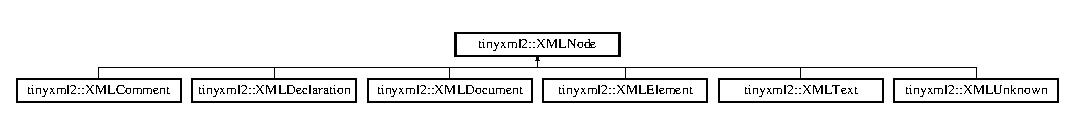
\includegraphics[height=1.145194cm]{classtinyxml2_1_1_x_m_l_node}
\end{center}
\end{figure}
\subsection*{Public Member Functions}
\begin{DoxyCompactItemize}
\item 
\hypertarget{classtinyxml2_1_1_x_m_l_node_add244bca368083fa29698db8dcf147ca}{const \hyperlink{classtinyxml2_1_1_x_m_l_document}{X\-M\-L\-Document} $\ast$ \hyperlink{classtinyxml2_1_1_x_m_l_node_add244bca368083fa29698db8dcf147ca}{Get\-Document} () const }\label{classtinyxml2_1_1_x_m_l_node_add244bca368083fa29698db8dcf147ca}

\begin{DoxyCompactList}\small\item\em Get the \hyperlink{classtinyxml2_1_1_x_m_l_document}{X\-M\-L\-Document} that owns this \hyperlink{classtinyxml2_1_1_x_m_l_node}{X\-M\-L\-Node}. \end{DoxyCompactList}\item 
\hypertarget{classtinyxml2_1_1_x_m_l_node_af343d1ef0b45c0020e62d784d7e67a68}{\hyperlink{classtinyxml2_1_1_x_m_l_document}{X\-M\-L\-Document} $\ast$ \hyperlink{classtinyxml2_1_1_x_m_l_node_af343d1ef0b45c0020e62d784d7e67a68}{Get\-Document} ()}\label{classtinyxml2_1_1_x_m_l_node_af343d1ef0b45c0020e62d784d7e67a68}

\begin{DoxyCompactList}\small\item\em Get the \hyperlink{classtinyxml2_1_1_x_m_l_document}{X\-M\-L\-Document} that owns this \hyperlink{classtinyxml2_1_1_x_m_l_node}{X\-M\-L\-Node}. \end{DoxyCompactList}\item 
\hypertarget{classtinyxml2_1_1_x_m_l_node_aab516e699567f75cc9ab2ef2eee501e8}{virtual \hyperlink{classtinyxml2_1_1_x_m_l_element}{X\-M\-L\-Element} $\ast$ \hyperlink{classtinyxml2_1_1_x_m_l_node_aab516e699567f75cc9ab2ef2eee501e8}{To\-Element} ()}\label{classtinyxml2_1_1_x_m_l_node_aab516e699567f75cc9ab2ef2eee501e8}

\begin{DoxyCompactList}\small\item\em Safely cast to an Element, or null. \end{DoxyCompactList}\item 
\hypertarget{classtinyxml2_1_1_x_m_l_node_a41c55dab9162d1eb62db2008430e376b}{virtual \hyperlink{classtinyxml2_1_1_x_m_l_text}{X\-M\-L\-Text} $\ast$ \hyperlink{classtinyxml2_1_1_x_m_l_node_a41c55dab9162d1eb62db2008430e376b}{To\-Text} ()}\label{classtinyxml2_1_1_x_m_l_node_a41c55dab9162d1eb62db2008430e376b}

\begin{DoxyCompactList}\small\item\em Safely cast to Text, or null. \end{DoxyCompactList}\item 
\hypertarget{classtinyxml2_1_1_x_m_l_node_aff47671055aa99840a1c1ebd661e63e3}{virtual \hyperlink{classtinyxml2_1_1_x_m_l_comment}{X\-M\-L\-Comment} $\ast$ \hyperlink{classtinyxml2_1_1_x_m_l_node_aff47671055aa99840a1c1ebd661e63e3}{To\-Comment} ()}\label{classtinyxml2_1_1_x_m_l_node_aff47671055aa99840a1c1ebd661e63e3}

\begin{DoxyCompactList}\small\item\em Safely cast to a Comment, or null. \end{DoxyCompactList}\item 
\hypertarget{classtinyxml2_1_1_x_m_l_node_a836e2966ed736fc3c94f70e12a2a3357}{virtual \hyperlink{classtinyxml2_1_1_x_m_l_document}{X\-M\-L\-Document} $\ast$ \hyperlink{classtinyxml2_1_1_x_m_l_node_a836e2966ed736fc3c94f70e12a2a3357}{To\-Document} ()}\label{classtinyxml2_1_1_x_m_l_node_a836e2966ed736fc3c94f70e12a2a3357}

\begin{DoxyCompactList}\small\item\em Safely cast to a Document, or null. \end{DoxyCompactList}\item 
\hypertarget{classtinyxml2_1_1_x_m_l_node_a174fd4c22c010b58138c1b84a0dfbd51}{virtual \hyperlink{classtinyxml2_1_1_x_m_l_declaration}{X\-M\-L\-Declaration} $\ast$ \hyperlink{classtinyxml2_1_1_x_m_l_node_a174fd4c22c010b58138c1b84a0dfbd51}{To\-Declaration} ()}\label{classtinyxml2_1_1_x_m_l_node_a174fd4c22c010b58138c1b84a0dfbd51}

\begin{DoxyCompactList}\small\item\em Safely cast to a Declaration, or null. \end{DoxyCompactList}\item 
\hypertarget{classtinyxml2_1_1_x_m_l_node_a8675a74aa0ada6eccab0c77ef3e5b9bd}{virtual \hyperlink{classtinyxml2_1_1_x_m_l_unknown}{X\-M\-L\-Unknown} $\ast$ \hyperlink{classtinyxml2_1_1_x_m_l_node_a8675a74aa0ada6eccab0c77ef3e5b9bd}{To\-Unknown} ()}\label{classtinyxml2_1_1_x_m_l_node_a8675a74aa0ada6eccab0c77ef3e5b9bd}

\begin{DoxyCompactList}\small\item\em Safely cast to an Unknown, or null. \end{DoxyCompactList}\item 
\hypertarget{classtinyxml2_1_1_x_m_l_node_acbaec609797ddabb4f9dcf38ee91262e}{virtual const \hyperlink{classtinyxml2_1_1_x_m_l_element}{X\-M\-L\-Element} $\ast$ {\bfseries To\-Element} () const }\label{classtinyxml2_1_1_x_m_l_node_acbaec609797ddabb4f9dcf38ee91262e}

\item 
\hypertarget{classtinyxml2_1_1_x_m_l_node_a89009ffc1b9f5d692bf8d4c9f18c3bec}{virtual const \hyperlink{classtinyxml2_1_1_x_m_l_text}{X\-M\-L\-Text} $\ast$ {\bfseries To\-Text} () const }\label{classtinyxml2_1_1_x_m_l_node_a89009ffc1b9f5d692bf8d4c9f18c3bec}

\item 
\hypertarget{classtinyxml2_1_1_x_m_l_node_a157ce3a00ea5ee5a85b7103138e85e8a}{virtual const \hyperlink{classtinyxml2_1_1_x_m_l_comment}{X\-M\-L\-Comment} $\ast$ {\bfseries To\-Comment} () const }\label{classtinyxml2_1_1_x_m_l_node_a157ce3a00ea5ee5a85b7103138e85e8a}

\item 
\hypertarget{classtinyxml2_1_1_x_m_l_node_a3ff975733a17d6ced3539b45544c8bf6}{virtual const \hyperlink{classtinyxml2_1_1_x_m_l_document}{X\-M\-L\-Document} $\ast$ {\bfseries To\-Document} () const }\label{classtinyxml2_1_1_x_m_l_node_a3ff975733a17d6ced3539b45544c8bf6}

\item 
\hypertarget{classtinyxml2_1_1_x_m_l_node_aedae0bbb58d533a4b8a61042388b49e5}{virtual const \hyperlink{classtinyxml2_1_1_x_m_l_declaration}{X\-M\-L\-Declaration} $\ast$ {\bfseries To\-Declaration} () const }\label{classtinyxml2_1_1_x_m_l_node_aedae0bbb58d533a4b8a61042388b49e5}

\item 
\hypertarget{classtinyxml2_1_1_x_m_l_node_a71f5ae90296dbe67979f83fe97073efa}{virtual const \hyperlink{classtinyxml2_1_1_x_m_l_unknown}{X\-M\-L\-Unknown} $\ast$ {\bfseries To\-Unknown} () const }\label{classtinyxml2_1_1_x_m_l_node_a71f5ae90296dbe67979f83fe97073efa}

\item 
const char $\ast$ \hyperlink{classtinyxml2_1_1_x_m_l_node_a7682be117e3b2b4ebfd517c1acaaadbf}{Value} () const 
\item 
void \hyperlink{classtinyxml2_1_1_x_m_l_node_a09dd68cf9eae137579f6e50f36487513}{Set\-Value} (const char $\ast$val, bool static\-Mem=false)
\item 
\hypertarget{classtinyxml2_1_1_x_m_l_node_a4e39bdcf9bfafa55d04857ece6aaf64e}{const \hyperlink{classtinyxml2_1_1_x_m_l_node}{X\-M\-L\-Node} $\ast$ \hyperlink{classtinyxml2_1_1_x_m_l_node_a4e39bdcf9bfafa55d04857ece6aaf64e}{Parent} () const }\label{classtinyxml2_1_1_x_m_l_node_a4e39bdcf9bfafa55d04857ece6aaf64e}

\begin{DoxyCompactList}\small\item\em Get the parent of this node on the D\-O\-M. \end{DoxyCompactList}\item 
\hypertarget{classtinyxml2_1_1_x_m_l_node_a76029693a5a54fbb721a41d7a0ca8a97}{\hyperlink{classtinyxml2_1_1_x_m_l_node}{X\-M\-L\-Node} $\ast$ {\bfseries Parent} ()}\label{classtinyxml2_1_1_x_m_l_node_a76029693a5a54fbb721a41d7a0ca8a97}

\item 
\hypertarget{classtinyxml2_1_1_x_m_l_node_a96afe34a9ccd0ed4c0cff32beb42cc6c}{bool \hyperlink{classtinyxml2_1_1_x_m_l_node_a96afe34a9ccd0ed4c0cff32beb42cc6c}{No\-Children} () const }\label{classtinyxml2_1_1_x_m_l_node_a96afe34a9ccd0ed4c0cff32beb42cc6c}

\begin{DoxyCompactList}\small\item\em Returns true if this node has no children. \end{DoxyCompactList}\item 
\hypertarget{classtinyxml2_1_1_x_m_l_node_a60e923d13d7dc01f45ab90a2f948b02a}{const \hyperlink{classtinyxml2_1_1_x_m_l_node}{X\-M\-L\-Node} $\ast$ \hyperlink{classtinyxml2_1_1_x_m_l_node_a60e923d13d7dc01f45ab90a2f948b02a}{First\-Child} () const }\label{classtinyxml2_1_1_x_m_l_node_a60e923d13d7dc01f45ab90a2f948b02a}

\begin{DoxyCompactList}\small\item\em Get the first child node, or null if none exists. \end{DoxyCompactList}\item 
\hypertarget{classtinyxml2_1_1_x_m_l_node_a2d6c70c475146b48bc93a7fafdeff5e0}{\hyperlink{classtinyxml2_1_1_x_m_l_node}{X\-M\-L\-Node} $\ast$ {\bfseries First\-Child} ()}\label{classtinyxml2_1_1_x_m_l_node_a2d6c70c475146b48bc93a7fafdeff5e0}

\item 
const \hyperlink{classtinyxml2_1_1_x_m_l_element}{X\-M\-L\-Element} $\ast$ \hyperlink{classtinyxml2_1_1_x_m_l_node_a20f48e99b03e9c17487944f229bee130}{First\-Child\-Element} (const char $\ast$value=0) const 
\item 
\hypertarget{classtinyxml2_1_1_x_m_l_node_a7614c3b4eea1ff11b2aa90b0f92f6dba}{\hyperlink{classtinyxml2_1_1_x_m_l_element}{X\-M\-L\-Element} $\ast$ {\bfseries First\-Child\-Element} (const char $\ast$value=0)}\label{classtinyxml2_1_1_x_m_l_node_a7614c3b4eea1ff11b2aa90b0f92f6dba}

\item 
\hypertarget{classtinyxml2_1_1_x_m_l_node_a6088246532b02895beb0e6fa561a7f3b}{const \hyperlink{classtinyxml2_1_1_x_m_l_node}{X\-M\-L\-Node} $\ast$ \hyperlink{classtinyxml2_1_1_x_m_l_node_a6088246532b02895beb0e6fa561a7f3b}{Last\-Child} () const }\label{classtinyxml2_1_1_x_m_l_node_a6088246532b02895beb0e6fa561a7f3b}

\begin{DoxyCompactList}\small\item\em Get the last child node, or null if none exists. \end{DoxyCompactList}\item 
\hypertarget{classtinyxml2_1_1_x_m_l_node_ad7552c8cb1dc0cb6f3bdc14a9d115dbf}{\hyperlink{classtinyxml2_1_1_x_m_l_node}{X\-M\-L\-Node} $\ast$ {\bfseries Last\-Child} ()}\label{classtinyxml2_1_1_x_m_l_node_ad7552c8cb1dc0cb6f3bdc14a9d115dbf}

\item 
const \hyperlink{classtinyxml2_1_1_x_m_l_element}{X\-M\-L\-Element} $\ast$ \hyperlink{classtinyxml2_1_1_x_m_l_node_a1a46cc01ece2216acf1e6294d1aff79d}{Last\-Child\-Element} (const char $\ast$value=0) const 
\item 
\hypertarget{classtinyxml2_1_1_x_m_l_node_a125423acf3170b130634638c5afc0639}{\hyperlink{classtinyxml2_1_1_x_m_l_element}{X\-M\-L\-Element} $\ast$ {\bfseries Last\-Child\-Element} (const char $\ast$value=0)}\label{classtinyxml2_1_1_x_m_l_node_a125423acf3170b130634638c5afc0639}

\item 
\hypertarget{classtinyxml2_1_1_x_m_l_node_a4cb1bf63e9de55129d21a7be60685fd4}{const \hyperlink{classtinyxml2_1_1_x_m_l_node}{X\-M\-L\-Node} $\ast$ \hyperlink{classtinyxml2_1_1_x_m_l_node_a4cb1bf63e9de55129d21a7be60685fd4}{Previous\-Sibling} () const }\label{classtinyxml2_1_1_x_m_l_node_a4cb1bf63e9de55129d21a7be60685fd4}

\begin{DoxyCompactList}\small\item\em Get the previous (left) sibling node of this node. \end{DoxyCompactList}\item 
\hypertarget{classtinyxml2_1_1_x_m_l_node_ae760e5e7e766df1d2cf3bb4a847876d6}{\hyperlink{classtinyxml2_1_1_x_m_l_node}{X\-M\-L\-Node} $\ast$ {\bfseries Previous\-Sibling} ()}\label{classtinyxml2_1_1_x_m_l_node_ae760e5e7e766df1d2cf3bb4a847876d6}

\item 
\hypertarget{classtinyxml2_1_1_x_m_l_node_a573b2559c41dce244d893d610fbe0bd9}{const \hyperlink{classtinyxml2_1_1_x_m_l_element}{X\-M\-L\-Element} $\ast$ \hyperlink{classtinyxml2_1_1_x_m_l_node_a573b2559c41dce244d893d610fbe0bd9}{Previous\-Sibling\-Element} (const char $\ast$value=0) const }\label{classtinyxml2_1_1_x_m_l_node_a573b2559c41dce244d893d610fbe0bd9}

\begin{DoxyCompactList}\small\item\em Get the previous (left) sibling element of this node, with an optionally supplied name. \end{DoxyCompactList}\item 
\hypertarget{classtinyxml2_1_1_x_m_l_node_ae9177fdc49cb89879f333581d5f734f1}{\hyperlink{classtinyxml2_1_1_x_m_l_element}{X\-M\-L\-Element} $\ast$ {\bfseries Previous\-Sibling\-Element} (const char $\ast$value=0)}\label{classtinyxml2_1_1_x_m_l_node_ae9177fdc49cb89879f333581d5f734f1}

\item 
\hypertarget{classtinyxml2_1_1_x_m_l_node_abba1df37581d89dccc45acdc55750ba2}{const \hyperlink{classtinyxml2_1_1_x_m_l_node}{X\-M\-L\-Node} $\ast$ \hyperlink{classtinyxml2_1_1_x_m_l_node_abba1df37581d89dccc45acdc55750ba2}{Next\-Sibling} () const }\label{classtinyxml2_1_1_x_m_l_node_abba1df37581d89dccc45acdc55750ba2}

\begin{DoxyCompactList}\small\item\em Get the next (right) sibling node of this node. \end{DoxyCompactList}\item 
\hypertarget{classtinyxml2_1_1_x_m_l_node_aeb7d4dfd8fb924ef86e7cb72183acbac}{\hyperlink{classtinyxml2_1_1_x_m_l_node}{X\-M\-L\-Node} $\ast$ {\bfseries Next\-Sibling} ()}\label{classtinyxml2_1_1_x_m_l_node_aeb7d4dfd8fb924ef86e7cb72183acbac}

\item 
\hypertarget{classtinyxml2_1_1_x_m_l_node_a490e166c3a1c6607960bfa9c112d3d30}{const \hyperlink{classtinyxml2_1_1_x_m_l_element}{X\-M\-L\-Element} $\ast$ \hyperlink{classtinyxml2_1_1_x_m_l_node_a490e166c3a1c6607960bfa9c112d3d30}{Next\-Sibling\-Element} (const char $\ast$value=0) const }\label{classtinyxml2_1_1_x_m_l_node_a490e166c3a1c6607960bfa9c112d3d30}

\begin{DoxyCompactList}\small\item\em Get the next (right) sibling element of this node, with an optionally supplied name. \end{DoxyCompactList}\item 
\hypertarget{classtinyxml2_1_1_x_m_l_node_acf735bf653016792522305d8ad4b3029}{\hyperlink{classtinyxml2_1_1_x_m_l_element}{X\-M\-L\-Element} $\ast$ {\bfseries Next\-Sibling\-Element} (const char $\ast$value=0)}\label{classtinyxml2_1_1_x_m_l_node_acf735bf653016792522305d8ad4b3029}

\item 
\hyperlink{classtinyxml2_1_1_x_m_l_node}{X\-M\-L\-Node} $\ast$ \hyperlink{classtinyxml2_1_1_x_m_l_node_ae3b422e98914d6002ca99bb1d2837103}{Insert\-End\-Child} (\hyperlink{classtinyxml2_1_1_x_m_l_node}{X\-M\-L\-Node} $\ast$add\-This)
\item 
\hypertarget{classtinyxml2_1_1_x_m_l_node_a663e3a5a378169fd477378f4d17a7649}{\hyperlink{classtinyxml2_1_1_x_m_l_node}{X\-M\-L\-Node} $\ast$ {\bfseries Link\-End\-Child} (\hyperlink{classtinyxml2_1_1_x_m_l_node}{X\-M\-L\-Node} $\ast$add\-This)}\label{classtinyxml2_1_1_x_m_l_node_a663e3a5a378169fd477378f4d17a7649}

\item 
\hyperlink{classtinyxml2_1_1_x_m_l_node}{X\-M\-L\-Node} $\ast$ \hyperlink{classtinyxml2_1_1_x_m_l_node_ac609a8f3ea949027f439280c640bbaf2}{Insert\-First\-Child} (\hyperlink{classtinyxml2_1_1_x_m_l_node}{X\-M\-L\-Node} $\ast$add\-This)
\item 
\hyperlink{classtinyxml2_1_1_x_m_l_node}{X\-M\-L\-Node} $\ast$ \hyperlink{classtinyxml2_1_1_x_m_l_node_a9275138a1b8dd5d8e2c26789bdc23ac8}{Insert\-After\-Child} (\hyperlink{classtinyxml2_1_1_x_m_l_node}{X\-M\-L\-Node} $\ast$after\-This, \hyperlink{classtinyxml2_1_1_x_m_l_node}{X\-M\-L\-Node} $\ast$add\-This)
\item 
void \hyperlink{classtinyxml2_1_1_x_m_l_node_a0360085cc54df5bff85d5c5da13afdce}{Delete\-Children} ()
\item 
void \hyperlink{classtinyxml2_1_1_x_m_l_node_a363b6edbd6ebd55f8387d2b89f2b0921}{Delete\-Child} (\hyperlink{classtinyxml2_1_1_x_m_l_node}{X\-M\-L\-Node} $\ast$node)
\item 
virtual \hyperlink{classtinyxml2_1_1_x_m_l_node}{X\-M\-L\-Node} $\ast$ \hyperlink{classtinyxml2_1_1_x_m_l_node_a8402cbd3129d20e9e6024bbcc0531283}{Shallow\-Clone} (\hyperlink{classtinyxml2_1_1_x_m_l_document}{X\-M\-L\-Document} $\ast$document) const =0
\item 
virtual bool \hyperlink{classtinyxml2_1_1_x_m_l_node_a7ce18b751c3ea09eac292dca264f9226}{Shallow\-Equal} (const \hyperlink{classtinyxml2_1_1_x_m_l_node}{X\-M\-L\-Node} $\ast$compare) const =0
\item 
virtual bool \hyperlink{classtinyxml2_1_1_x_m_l_node_a81e66df0a44c67a7af17f3b77a152785}{Accept} (\hyperlink{classtinyxml2_1_1_x_m_l_visitor}{X\-M\-L\-Visitor} $\ast$visitor) const =0
\item 
\hypertarget{classtinyxml2_1_1_x_m_l_node_a7610d0f603e8b603d2078521811a23c1}{virtual char $\ast$ {\bfseries Parse\-Deep} (char $\ast$, \hyperlink{classtinyxml2_1_1_str_pair}{Str\-Pair} $\ast$)}\label{classtinyxml2_1_1_x_m_l_node_a7610d0f603e8b603d2078521811a23c1}

\end{DoxyCompactItemize}
\subsection*{Protected Member Functions}
\begin{DoxyCompactItemize}
\item 
\hypertarget{classtinyxml2_1_1_x_m_l_node_a29868df6ca383d574f584dfdd15105b6}{{\bfseries X\-M\-L\-Node} (\hyperlink{classtinyxml2_1_1_x_m_l_document}{X\-M\-L\-Document} $\ast$)}\label{classtinyxml2_1_1_x_m_l_node_a29868df6ca383d574f584dfdd15105b6}

\item 
\hypertarget{classtinyxml2_1_1_x_m_l_node_a78be01384518a969da905548f318d75b}{{\bfseries X\-M\-L\-Node} (const \hyperlink{classtinyxml2_1_1_x_m_l_node}{X\-M\-L\-Node} \&)}\label{classtinyxml2_1_1_x_m_l_node_a78be01384518a969da905548f318d75b}

\item 
\hypertarget{classtinyxml2_1_1_x_m_l_node_ade79231d908e1f21862819e00e56ab6e}{\hyperlink{classtinyxml2_1_1_x_m_l_node}{X\-M\-L\-Node} \& {\bfseries operator=} (const \hyperlink{classtinyxml2_1_1_x_m_l_node}{X\-M\-L\-Node} \&)}\label{classtinyxml2_1_1_x_m_l_node_ade79231d908e1f21862819e00e56ab6e}

\end{DoxyCompactItemize}
\subsection*{Protected Attributes}
\begin{DoxyCompactItemize}
\item 
\hypertarget{classtinyxml2_1_1_x_m_l_node_a8d2d2be0bb6797625551eb0e91f0ff62}{\hyperlink{classtinyxml2_1_1_x_m_l_document}{X\-M\-L\-Document} $\ast$ {\bfseries \-\_\-document}}\label{classtinyxml2_1_1_x_m_l_node_a8d2d2be0bb6797625551eb0e91f0ff62}

\item 
\hypertarget{classtinyxml2_1_1_x_m_l_node_a176dd1c4965c21c366de192164aa2c13}{\hyperlink{classtinyxml2_1_1_x_m_l_node}{X\-M\-L\-Node} $\ast$ {\bfseries \-\_\-parent}}\label{classtinyxml2_1_1_x_m_l_node_a176dd1c4965c21c366de192164aa2c13}

\item 
\hypertarget{classtinyxml2_1_1_x_m_l_node_a3ea9884098b8379de2bb5ab3fc85c0fc}{\hyperlink{classtinyxml2_1_1_str_pair}{Str\-Pair} {\bfseries \-\_\-value}}\label{classtinyxml2_1_1_x_m_l_node_a3ea9884098b8379de2bb5ab3fc85c0fc}

\item 
\hypertarget{classtinyxml2_1_1_x_m_l_node_aa20c91e4213dc930c5bdf420322ca342}{\hyperlink{classtinyxml2_1_1_x_m_l_node}{X\-M\-L\-Node} $\ast$ {\bfseries \-\_\-first\-Child}}\label{classtinyxml2_1_1_x_m_l_node_aa20c91e4213dc930c5bdf420322ca342}

\item 
\hypertarget{classtinyxml2_1_1_x_m_l_node_a099b6560ae44ab9edb8453aaf1a3747b}{\hyperlink{classtinyxml2_1_1_x_m_l_node}{X\-M\-L\-Node} $\ast$ {\bfseries \-\_\-last\-Child}}\label{classtinyxml2_1_1_x_m_l_node_a099b6560ae44ab9edb8453aaf1a3747b}

\item 
\hypertarget{classtinyxml2_1_1_x_m_l_node_a9739eb0fb9a1188266052055e7a6bf6b}{\hyperlink{classtinyxml2_1_1_x_m_l_node}{X\-M\-L\-Node} $\ast$ {\bfseries \-\_\-prev}}\label{classtinyxml2_1_1_x_m_l_node_a9739eb0fb9a1188266052055e7a6bf6b}

\item 
\hypertarget{classtinyxml2_1_1_x_m_l_node_a27e985496b37dd00eb5b9cf59b9e3fb1}{\hyperlink{classtinyxml2_1_1_x_m_l_node}{X\-M\-L\-Node} $\ast$ {\bfseries \-\_\-next}}\label{classtinyxml2_1_1_x_m_l_node_a27e985496b37dd00eb5b9cf59b9e3fb1}

\end{DoxyCompactItemize}
\subsection*{Friends}
\begin{DoxyCompactItemize}
\item 
\hypertarget{classtinyxml2_1_1_x_m_l_node_a4eee3bda60c60a30e4e8cd4ea91c4c6e}{class {\bfseries X\-M\-L\-Document}}\label{classtinyxml2_1_1_x_m_l_node_a4eee3bda60c60a30e4e8cd4ea91c4c6e}

\item 
\hypertarget{classtinyxml2_1_1_x_m_l_node_ac2fba9b6e452829dd892f7392c24e0eb}{class {\bfseries X\-M\-L\-Element}}\label{classtinyxml2_1_1_x_m_l_node_ac2fba9b6e452829dd892f7392c24e0eb}

\end{DoxyCompactItemize}


\subsection{Detailed Description}
\hyperlink{classtinyxml2_1_1_x_m_l_node}{X\-M\-L\-Node} is a base class for every object that is in the X\-M\-L Document Object Model (D\-O\-M), except X\-M\-L\-Attributes. Nodes have siblings, a parent, and children which can be navigated. A node is always in a \hyperlink{classtinyxml2_1_1_x_m_l_document}{X\-M\-L\-Document}. The type of a \hyperlink{classtinyxml2_1_1_x_m_l_node}{X\-M\-L\-Node} can be queried, and it can be cast to its more defined type.

A \hyperlink{classtinyxml2_1_1_x_m_l_document}{X\-M\-L\-Document} allocates memory for all its Nodes. When the \hyperlink{classtinyxml2_1_1_x_m_l_document}{X\-M\-L\-Document} gets deleted, all its Nodes will also be deleted.

\begin{DoxyVerb}A Document can contain: Element (container or leaf)
                        Comment (leaf)
                        Unknown (leaf)
                        Declaration( leaf )

An Element can contain: Element (container or leaf)
                        Text    (leaf)
                        Attributes (not on tree)
                        Comment (leaf)
                        Unknown (leaf)\end{DoxyVerb}
 

\subsection{Member Function Documentation}
\hypertarget{classtinyxml2_1_1_x_m_l_node_a81e66df0a44c67a7af17f3b77a152785}{\index{tinyxml2\-::\-X\-M\-L\-Node@{tinyxml2\-::\-X\-M\-L\-Node}!Accept@{Accept}}
\index{Accept@{Accept}!tinyxml2::XMLNode@{tinyxml2\-::\-X\-M\-L\-Node}}
\subsubsection[{Accept}]{\setlength{\rightskip}{0pt plus 5cm}virtual bool tinyxml2\-::\-X\-M\-L\-Node\-::\-Accept (
\begin{DoxyParamCaption}
\item[{{\bf X\-M\-L\-Visitor} $\ast$}]{visitor}
\end{DoxyParamCaption}
) const\hspace{0.3cm}{\ttfamily [pure virtual]}}}\label{classtinyxml2_1_1_x_m_l_node_a81e66df0a44c67a7af17f3b77a152785}
Accept a hierarchical visit of the nodes in the Tiny\-X\-M\-L-\/2 D\-O\-M. Every node in the X\-M\-L tree will be conditionally visited and the host will be called back via the \hyperlink{classtinyxml2_1_1_x_m_l_visitor}{X\-M\-L\-Visitor} interface.

This is essentially a S\-A\-X interface for Tiny\-X\-M\-L-\/2. (Note however it doesn't re-\/parse the X\-M\-L for the callbacks, so the performance of Tiny\-X\-M\-L-\/2 is unchanged by using this interface versus any other.)

The interface has been based on ideas from\-:


\begin{DoxyItemize}
\item \href{http://www.saxproject.org/}{\tt http\-://www.\-saxproject.\-org/}
\item \href{http://c2.com/cgi/wiki?HierarchicalVisitorPattern}{\tt http\-://c2.\-com/cgi/wiki?\-Hierarchical\-Visitor\-Pattern}
\end{DoxyItemize}

Which are both good references for \char`\"{}visiting\char`\"{}.

An example of using \hyperlink{classtinyxml2_1_1_x_m_l_node_a81e66df0a44c67a7af17f3b77a152785}{Accept()}\-: \begin{DoxyVerb}XMLPrinter printer;
tinyxmlDoc.Accept( &printer );
const char* xmlcstr = printer.CStr();
\end{DoxyVerb}
 

Implemented in \hyperlink{classtinyxml2_1_1_x_m_l_document_aa08503d24898bf9992ae5e5fb8b0cf87}{tinyxml2\-::\-X\-M\-L\-Document}, \hyperlink{classtinyxml2_1_1_x_m_l_element_a36d65438991a1e85096caf39ad13a099}{tinyxml2\-::\-X\-M\-L\-Element}, \hyperlink{classtinyxml2_1_1_x_m_l_unknown_a0d341ab804a1438a474810bb5bd29dd5}{tinyxml2\-::\-X\-M\-L\-Unknown}, \hyperlink{classtinyxml2_1_1_x_m_l_declaration_a953a7359cc312d15218eb5843a4ca108}{tinyxml2\-::\-X\-M\-L\-Declaration}, \hyperlink{classtinyxml2_1_1_x_m_l_comment_aa382b1be6a8b0650c16a2d88bb499335}{tinyxml2\-::\-X\-M\-L\-Comment}, and \hyperlink{classtinyxml2_1_1_x_m_l_text_ae659d4fc7351a7df11c111cbe1ade46f}{tinyxml2\-::\-X\-M\-L\-Text}.

\hypertarget{classtinyxml2_1_1_x_m_l_node_a363b6edbd6ebd55f8387d2b89f2b0921}{\index{tinyxml2\-::\-X\-M\-L\-Node@{tinyxml2\-::\-X\-M\-L\-Node}!Delete\-Child@{Delete\-Child}}
\index{Delete\-Child@{Delete\-Child}!tinyxml2::XMLNode@{tinyxml2\-::\-X\-M\-L\-Node}}
\subsubsection[{Delete\-Child}]{\setlength{\rightskip}{0pt plus 5cm}void tinyxml2\-::\-X\-M\-L\-Node\-::\-Delete\-Child (
\begin{DoxyParamCaption}
\item[{{\bf X\-M\-L\-Node} $\ast$}]{node}
\end{DoxyParamCaption}
)}}\label{classtinyxml2_1_1_x_m_l_node_a363b6edbd6ebd55f8387d2b89f2b0921}
Delete a child of this node. \hypertarget{classtinyxml2_1_1_x_m_l_node_a0360085cc54df5bff85d5c5da13afdce}{\index{tinyxml2\-::\-X\-M\-L\-Node@{tinyxml2\-::\-X\-M\-L\-Node}!Delete\-Children@{Delete\-Children}}
\index{Delete\-Children@{Delete\-Children}!tinyxml2::XMLNode@{tinyxml2\-::\-X\-M\-L\-Node}}
\subsubsection[{Delete\-Children}]{\setlength{\rightskip}{0pt plus 5cm}void tinyxml2\-::\-X\-M\-L\-Node\-::\-Delete\-Children (
\begin{DoxyParamCaption}
{}
\end{DoxyParamCaption}
)}}\label{classtinyxml2_1_1_x_m_l_node_a0360085cc54df5bff85d5c5da13afdce}
Delete all the children of this node. \hypertarget{classtinyxml2_1_1_x_m_l_node_a20f48e99b03e9c17487944f229bee130}{\index{tinyxml2\-::\-X\-M\-L\-Node@{tinyxml2\-::\-X\-M\-L\-Node}!First\-Child\-Element@{First\-Child\-Element}}
\index{First\-Child\-Element@{First\-Child\-Element}!tinyxml2::XMLNode@{tinyxml2\-::\-X\-M\-L\-Node}}
\subsubsection[{First\-Child\-Element}]{\setlength{\rightskip}{0pt plus 5cm}const {\bf X\-M\-L\-Element} $\ast$ tinyxml2\-::\-X\-M\-L\-Node\-::\-First\-Child\-Element (
\begin{DoxyParamCaption}
\item[{const char $\ast$}]{value = {\ttfamily 0}}
\end{DoxyParamCaption}
) const}}\label{classtinyxml2_1_1_x_m_l_node_a20f48e99b03e9c17487944f229bee130}
Get the first child element, or optionally the first child element with the specified name. \hypertarget{classtinyxml2_1_1_x_m_l_node_a9275138a1b8dd5d8e2c26789bdc23ac8}{\index{tinyxml2\-::\-X\-M\-L\-Node@{tinyxml2\-::\-X\-M\-L\-Node}!Insert\-After\-Child@{Insert\-After\-Child}}
\index{Insert\-After\-Child@{Insert\-After\-Child}!tinyxml2::XMLNode@{tinyxml2\-::\-X\-M\-L\-Node}}
\subsubsection[{Insert\-After\-Child}]{\setlength{\rightskip}{0pt plus 5cm}{\bf X\-M\-L\-Node} $\ast$ tinyxml2\-::\-X\-M\-L\-Node\-::\-Insert\-After\-Child (
\begin{DoxyParamCaption}
\item[{{\bf X\-M\-L\-Node} $\ast$}]{after\-This, }
\item[{{\bf X\-M\-L\-Node} $\ast$}]{add\-This}
\end{DoxyParamCaption}
)}}\label{classtinyxml2_1_1_x_m_l_node_a9275138a1b8dd5d8e2c26789bdc23ac8}
Add a node after the specified child node. \hypertarget{classtinyxml2_1_1_x_m_l_node_ae3b422e98914d6002ca99bb1d2837103}{\index{tinyxml2\-::\-X\-M\-L\-Node@{tinyxml2\-::\-X\-M\-L\-Node}!Insert\-End\-Child@{Insert\-End\-Child}}
\index{Insert\-End\-Child@{Insert\-End\-Child}!tinyxml2::XMLNode@{tinyxml2\-::\-X\-M\-L\-Node}}
\subsubsection[{Insert\-End\-Child}]{\setlength{\rightskip}{0pt plus 5cm}{\bf X\-M\-L\-Node} $\ast$ tinyxml2\-::\-X\-M\-L\-Node\-::\-Insert\-End\-Child (
\begin{DoxyParamCaption}
\item[{{\bf X\-M\-L\-Node} $\ast$}]{add\-This}
\end{DoxyParamCaption}
)}}\label{classtinyxml2_1_1_x_m_l_node_ae3b422e98914d6002ca99bb1d2837103}
Add a child node as the last (right) child. \hypertarget{classtinyxml2_1_1_x_m_l_node_ac609a8f3ea949027f439280c640bbaf2}{\index{tinyxml2\-::\-X\-M\-L\-Node@{tinyxml2\-::\-X\-M\-L\-Node}!Insert\-First\-Child@{Insert\-First\-Child}}
\index{Insert\-First\-Child@{Insert\-First\-Child}!tinyxml2::XMLNode@{tinyxml2\-::\-X\-M\-L\-Node}}
\subsubsection[{Insert\-First\-Child}]{\setlength{\rightskip}{0pt plus 5cm}{\bf X\-M\-L\-Node} $\ast$ tinyxml2\-::\-X\-M\-L\-Node\-::\-Insert\-First\-Child (
\begin{DoxyParamCaption}
\item[{{\bf X\-M\-L\-Node} $\ast$}]{add\-This}
\end{DoxyParamCaption}
)}}\label{classtinyxml2_1_1_x_m_l_node_ac609a8f3ea949027f439280c640bbaf2}
Add a child node as the first (left) child. \hypertarget{classtinyxml2_1_1_x_m_l_node_a1a46cc01ece2216acf1e6294d1aff79d}{\index{tinyxml2\-::\-X\-M\-L\-Node@{tinyxml2\-::\-X\-M\-L\-Node}!Last\-Child\-Element@{Last\-Child\-Element}}
\index{Last\-Child\-Element@{Last\-Child\-Element}!tinyxml2::XMLNode@{tinyxml2\-::\-X\-M\-L\-Node}}
\subsubsection[{Last\-Child\-Element}]{\setlength{\rightskip}{0pt plus 5cm}const {\bf X\-M\-L\-Element} $\ast$ tinyxml2\-::\-X\-M\-L\-Node\-::\-Last\-Child\-Element (
\begin{DoxyParamCaption}
\item[{const char $\ast$}]{value = {\ttfamily 0}}
\end{DoxyParamCaption}
) const}}\label{classtinyxml2_1_1_x_m_l_node_a1a46cc01ece2216acf1e6294d1aff79d}
Get the last child element or optionally the last child element with the specified name. \hypertarget{classtinyxml2_1_1_x_m_l_node_a09dd68cf9eae137579f6e50f36487513}{\index{tinyxml2\-::\-X\-M\-L\-Node@{tinyxml2\-::\-X\-M\-L\-Node}!Set\-Value@{Set\-Value}}
\index{Set\-Value@{Set\-Value}!tinyxml2::XMLNode@{tinyxml2\-::\-X\-M\-L\-Node}}
\subsubsection[{Set\-Value}]{\setlength{\rightskip}{0pt plus 5cm}void tinyxml2\-::\-X\-M\-L\-Node\-::\-Set\-Value (
\begin{DoxyParamCaption}
\item[{const char $\ast$}]{val, }
\item[{bool}]{static\-Mem = {\ttfamily false}}
\end{DoxyParamCaption}
)}}\label{classtinyxml2_1_1_x_m_l_node_a09dd68cf9eae137579f6e50f36487513}
Set the Value of an X\-M\-L node. \begin{DoxySeeAlso}{See Also}
\hyperlink{classtinyxml2_1_1_x_m_l_node_a7682be117e3b2b4ebfd517c1acaaadbf}{Value()} 
\end{DoxySeeAlso}
\hypertarget{classtinyxml2_1_1_x_m_l_node_a8402cbd3129d20e9e6024bbcc0531283}{\index{tinyxml2\-::\-X\-M\-L\-Node@{tinyxml2\-::\-X\-M\-L\-Node}!Shallow\-Clone@{Shallow\-Clone}}
\index{Shallow\-Clone@{Shallow\-Clone}!tinyxml2::XMLNode@{tinyxml2\-::\-X\-M\-L\-Node}}
\subsubsection[{Shallow\-Clone}]{\setlength{\rightskip}{0pt plus 5cm}virtual {\bf X\-M\-L\-Node}$\ast$ tinyxml2\-::\-X\-M\-L\-Node\-::\-Shallow\-Clone (
\begin{DoxyParamCaption}
\item[{{\bf X\-M\-L\-Document} $\ast$}]{document}
\end{DoxyParamCaption}
) const\hspace{0.3cm}{\ttfamily [pure virtual]}}}\label{classtinyxml2_1_1_x_m_l_node_a8402cbd3129d20e9e6024bbcc0531283}
Make a copy of this node, but not its children. You may pass in a Document pointer that will be the owner of the new Node. If the 'document' is null, then the node returned will be allocated from the current Document. (this-\/$>$\hyperlink{classtinyxml2_1_1_x_m_l_node_af343d1ef0b45c0020e62d784d7e67a68}{Get\-Document()})

Note\-: if called on a \hyperlink{classtinyxml2_1_1_x_m_l_document}{X\-M\-L\-Document}, this will return null. 

Implemented in \hyperlink{classtinyxml2_1_1_x_m_l_document_a57c8511ed9f83aa3e20909a3db3f83d0}{tinyxml2\-::\-X\-M\-L\-Document}, \hyperlink{classtinyxml2_1_1_x_m_l_element_a85d85e32c18863fff1eeed53ae1ce23d}{tinyxml2\-::\-X\-M\-L\-Element}, \hyperlink{classtinyxml2_1_1_x_m_l_unknown_aa09fc7cb0cd64d6bb9c5ae00ffc549ec}{tinyxml2\-::\-X\-M\-L\-Unknown}, \hyperlink{classtinyxml2_1_1_x_m_l_declaration_a39458732ee6796cfc85dd35d3c488e0b}{tinyxml2\-::\-X\-M\-L\-Declaration}, \hyperlink{classtinyxml2_1_1_x_m_l_comment_a90bb60193a691b484f5e1b487857016d}{tinyxml2\-::\-X\-M\-L\-Comment}, and \hyperlink{classtinyxml2_1_1_x_m_l_text_af5115f8cc83de2947ed6a9d13e2f88c8}{tinyxml2\-::\-X\-M\-L\-Text}.

\hypertarget{classtinyxml2_1_1_x_m_l_node_a7ce18b751c3ea09eac292dca264f9226}{\index{tinyxml2\-::\-X\-M\-L\-Node@{tinyxml2\-::\-X\-M\-L\-Node}!Shallow\-Equal@{Shallow\-Equal}}
\index{Shallow\-Equal@{Shallow\-Equal}!tinyxml2::XMLNode@{tinyxml2\-::\-X\-M\-L\-Node}}
\subsubsection[{Shallow\-Equal}]{\setlength{\rightskip}{0pt plus 5cm}virtual bool tinyxml2\-::\-X\-M\-L\-Node\-::\-Shallow\-Equal (
\begin{DoxyParamCaption}
\item[{const {\bf X\-M\-L\-Node} $\ast$}]{compare}
\end{DoxyParamCaption}
) const\hspace{0.3cm}{\ttfamily [pure virtual]}}}\label{classtinyxml2_1_1_x_m_l_node_a7ce18b751c3ea09eac292dca264f9226}
Test if 2 nodes are the same, but don't test children. The 2 nodes do not need to be in the same Document.

Note\-: if called on a \hyperlink{classtinyxml2_1_1_x_m_l_document}{X\-M\-L\-Document}, this will return false. 

Implemented in \hyperlink{classtinyxml2_1_1_x_m_l_document_a12eac66c6e45d074d5cc47319868cd66}{tinyxml2\-::\-X\-M\-L\-Document}, \hyperlink{classtinyxml2_1_1_x_m_l_element_a25d51a2aad92625c78441457d58c85bc}{tinyxml2\-::\-X\-M\-L\-Element}, \hyperlink{classtinyxml2_1_1_x_m_l_unknown_a0169df157bf69a092b404ca49621ff1a}{tinyxml2\-::\-X\-M\-L\-Unknown}, \hyperlink{classtinyxml2_1_1_x_m_l_declaration_ace0d2d9bc1b63278bd5e984ebe0c7bd0}{tinyxml2\-::\-X\-M\-L\-Declaration}, \hyperlink{classtinyxml2_1_1_x_m_l_comment_a2d9f26757b0018fce933e74420cda22a}{tinyxml2\-::\-X\-M\-L\-Comment}, and \hyperlink{classtinyxml2_1_1_x_m_l_text_a1588aa5d23cb21eb31f36df0aaaa8d66}{tinyxml2\-::\-X\-M\-L\-Text}.

\hypertarget{classtinyxml2_1_1_x_m_l_node_a7682be117e3b2b4ebfd517c1acaaadbf}{\index{tinyxml2\-::\-X\-M\-L\-Node@{tinyxml2\-::\-X\-M\-L\-Node}!Value@{Value}}
\index{Value@{Value}!tinyxml2::XMLNode@{tinyxml2\-::\-X\-M\-L\-Node}}
\subsubsection[{Value}]{\setlength{\rightskip}{0pt plus 5cm}const char$\ast$ tinyxml2\-::\-X\-M\-L\-Node\-::\-Value (
\begin{DoxyParamCaption}
{}
\end{DoxyParamCaption}
) const\hspace{0.3cm}{\ttfamily [inline]}}}\label{classtinyxml2_1_1_x_m_l_node_a7682be117e3b2b4ebfd517c1acaaadbf}
The meaning of 'value' changes for the specific type. \begin{DoxyVerb}Document:   empty
Element:    name of the element
Comment:    the comment text
Unknown:    the tag contents
Text:       the text string
\end{DoxyVerb}
 

The documentation for this class was generated from the following files\-:\begin{DoxyCompactItemize}
\item 
tinyxml2.\-h\item 
tinyxml2.\-cpp\end{DoxyCompactItemize}

\hypertarget{classtinyxml2_1_1_x_m_l_printer}{\section{tinyxml2\-:\-:X\-M\-L\-Printer Class Reference}
\label{classtinyxml2_1_1_x_m_l_printer}\index{tinyxml2\-::\-X\-M\-L\-Printer@{tinyxml2\-::\-X\-M\-L\-Printer}}
}


{\ttfamily \#include $<$tinyxml2.\-h$>$}

Inheritance diagram for tinyxml2\-:\-:X\-M\-L\-Printer\-:\begin{figure}[H]
\begin{center}
\leavevmode
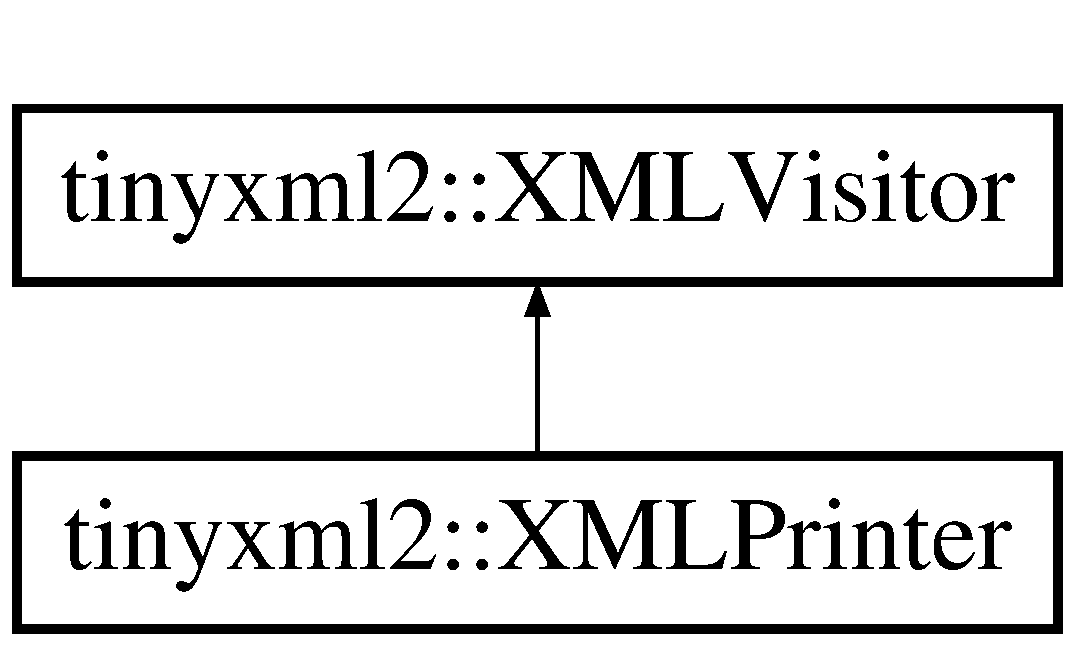
\includegraphics[height=2.000000cm]{classtinyxml2_1_1_x_m_l_printer}
\end{center}
\end{figure}
\subsection*{Public Member Functions}
\begin{DoxyCompactItemize}
\item 
\hyperlink{classtinyxml2_1_1_x_m_l_printer_ad1eb8de568ceac1429cf04c66a349bd6}{X\-M\-L\-Printer} (F\-I\-L\-E $\ast$file=0, bool compact=false)
\item 
void \hyperlink{classtinyxml2_1_1_x_m_l_printer_a178c608ce8476043d5d6513819cde903}{Push\-Header} (bool write\-B\-O\-M, bool write\-Declaration)
\item 
void \hyperlink{classtinyxml2_1_1_x_m_l_printer_aa10d330818dbc31b44e9ffc27618bdfb}{Open\-Element} (const char $\ast$name)
\item 
\hypertarget{classtinyxml2_1_1_x_m_l_printer_a9a4e2c9348b42e147629d5a99f4af3f0}{void \hyperlink{classtinyxml2_1_1_x_m_l_printer_a9a4e2c9348b42e147629d5a99f4af3f0}{Push\-Attribute} (const char $\ast$name, const char $\ast$value)}\label{classtinyxml2_1_1_x_m_l_printer_a9a4e2c9348b42e147629d5a99f4af3f0}

\begin{DoxyCompactList}\small\item\em If streaming, add an attribute to an open element. \end{DoxyCompactList}\item 
\hypertarget{classtinyxml2_1_1_x_m_l_printer_a69120c82088597372d28d0a98f2ee7a1}{void {\bfseries Push\-Attribute} (const char $\ast$name, int value)}\label{classtinyxml2_1_1_x_m_l_printer_a69120c82088597372d28d0a98f2ee7a1}

\item 
\hypertarget{classtinyxml2_1_1_x_m_l_printer_aa41039e51990aaf5342f3e0575a692c4}{void {\bfseries Push\-Attribute} (const char $\ast$name, unsigned value)}\label{classtinyxml2_1_1_x_m_l_printer_aa41039e51990aaf5342f3e0575a692c4}

\item 
\hypertarget{classtinyxml2_1_1_x_m_l_printer_a51f7950d7b7a19f0d3a0d549a318d45f}{void {\bfseries Push\-Attribute} (const char $\ast$name, bool value)}\label{classtinyxml2_1_1_x_m_l_printer_a51f7950d7b7a19f0d3a0d549a318d45f}

\item 
\hypertarget{classtinyxml2_1_1_x_m_l_printer_a1714867af40e68ca404c3e84b6cac2a6}{void {\bfseries Push\-Attribute} (const char $\ast$name, double value)}\label{classtinyxml2_1_1_x_m_l_printer_a1714867af40e68ca404c3e84b6cac2a6}

\item 
\hypertarget{classtinyxml2_1_1_x_m_l_printer_aed6cce4bd414a78b3e2a824803c3ec42}{void \hyperlink{classtinyxml2_1_1_x_m_l_printer_aed6cce4bd414a78b3e2a824803c3ec42}{Close\-Element} ()}\label{classtinyxml2_1_1_x_m_l_printer_aed6cce4bd414a78b3e2a824803c3ec42}

\begin{DoxyCompactList}\small\item\em If streaming, close the Element. \end{DoxyCompactList}\item 
\hypertarget{classtinyxml2_1_1_x_m_l_printer_a1cc16a9362df4332012cb13cff6441b3}{void \hyperlink{classtinyxml2_1_1_x_m_l_printer_a1cc16a9362df4332012cb13cff6441b3}{Push\-Text} (const char $\ast$text, bool cdata=false)}\label{classtinyxml2_1_1_x_m_l_printer_a1cc16a9362df4332012cb13cff6441b3}

\begin{DoxyCompactList}\small\item\em Add a text node. \end{DoxyCompactList}\item 
\hypertarget{classtinyxml2_1_1_x_m_l_printer_a3e0d4d78de25d4cf081009e1431cea7e}{void \hyperlink{classtinyxml2_1_1_x_m_l_printer_a3e0d4d78de25d4cf081009e1431cea7e}{Push\-Text} (int value)}\label{classtinyxml2_1_1_x_m_l_printer_a3e0d4d78de25d4cf081009e1431cea7e}

\begin{DoxyCompactList}\small\item\em Add a text node from an integer. \end{DoxyCompactList}\item 
\hypertarget{classtinyxml2_1_1_x_m_l_printer_a661fb50e7e0a4918d2d259cb0fae647e}{void \hyperlink{classtinyxml2_1_1_x_m_l_printer_a661fb50e7e0a4918d2d259cb0fae647e}{Push\-Text} (unsigned value)}\label{classtinyxml2_1_1_x_m_l_printer_a661fb50e7e0a4918d2d259cb0fae647e}

\begin{DoxyCompactList}\small\item\em Add a text node from an unsigned. \end{DoxyCompactList}\item 
\hypertarget{classtinyxml2_1_1_x_m_l_printer_a4390e5fa1ed05189a8686647345ab29f}{void \hyperlink{classtinyxml2_1_1_x_m_l_printer_a4390e5fa1ed05189a8686647345ab29f}{Push\-Text} (bool value)}\label{classtinyxml2_1_1_x_m_l_printer_a4390e5fa1ed05189a8686647345ab29f}

\begin{DoxyCompactList}\small\item\em Add a text node from a bool. \end{DoxyCompactList}\item 
\hypertarget{classtinyxml2_1_1_x_m_l_printer_a1dbb1390e829d0673af66b9cd1928bd7}{void \hyperlink{classtinyxml2_1_1_x_m_l_printer_a1dbb1390e829d0673af66b9cd1928bd7}{Push\-Text} (float value)}\label{classtinyxml2_1_1_x_m_l_printer_a1dbb1390e829d0673af66b9cd1928bd7}

\begin{DoxyCompactList}\small\item\em Add a text node from a float. \end{DoxyCompactList}\item 
\hypertarget{classtinyxml2_1_1_x_m_l_printer_aa715302dfc09473c77c853cbd5431965}{void \hyperlink{classtinyxml2_1_1_x_m_l_printer_aa715302dfc09473c77c853cbd5431965}{Push\-Text} (double value)}\label{classtinyxml2_1_1_x_m_l_printer_aa715302dfc09473c77c853cbd5431965}

\begin{DoxyCompactList}\small\item\em Add a text node from a double. \end{DoxyCompactList}\item 
\hypertarget{classtinyxml2_1_1_x_m_l_printer_afc8416814219591c2fd5656e0c233140}{void \hyperlink{classtinyxml2_1_1_x_m_l_printer_afc8416814219591c2fd5656e0c233140}{Push\-Comment} (const char $\ast$comment)}\label{classtinyxml2_1_1_x_m_l_printer_afc8416814219591c2fd5656e0c233140}

\begin{DoxyCompactList}\small\item\em Add a comment. \end{DoxyCompactList}\item 
\hypertarget{classtinyxml2_1_1_x_m_l_printer_a2fe3565e262594efc6c0276723c83fe7}{void {\bfseries Push\-Declaration} (const char $\ast$value)}\label{classtinyxml2_1_1_x_m_l_printer_a2fe3565e262594efc6c0276723c83fe7}

\item 
\hypertarget{classtinyxml2_1_1_x_m_l_printer_ab1efc6d1548505e9984185f58f54b713}{void {\bfseries Push\-Unknown} (const char $\ast$value)}\label{classtinyxml2_1_1_x_m_l_printer_ab1efc6d1548505e9984185f58f54b713}

\item 
\hypertarget{classtinyxml2_1_1_x_m_l_printer_a9aa1de11a55a07db55a90fde37d7afad}{virtual bool \hyperlink{classtinyxml2_1_1_x_m_l_printer_a9aa1de11a55a07db55a90fde37d7afad}{Visit\-Enter} (const \hyperlink{classtinyxml2_1_1_x_m_l_document}{X\-M\-L\-Document} \&)}\label{classtinyxml2_1_1_x_m_l_printer_a9aa1de11a55a07db55a90fde37d7afad}

\begin{DoxyCompactList}\small\item\em Visit a document. \end{DoxyCompactList}\item 
\hypertarget{classtinyxml2_1_1_x_m_l_printer_a15fc1f2b922f540917dcf52808737b29}{virtual bool \hyperlink{classtinyxml2_1_1_x_m_l_printer_a15fc1f2b922f540917dcf52808737b29}{Visit\-Exit} (const \hyperlink{classtinyxml2_1_1_x_m_l_document}{X\-M\-L\-Document} \&)}\label{classtinyxml2_1_1_x_m_l_printer_a15fc1f2b922f540917dcf52808737b29}

\begin{DoxyCompactList}\small\item\em Visit a document. \end{DoxyCompactList}\item 
\hypertarget{classtinyxml2_1_1_x_m_l_printer_a169b2509d8eabb70811b2bb8cfd1f5d1}{virtual bool \hyperlink{classtinyxml2_1_1_x_m_l_printer_a169b2509d8eabb70811b2bb8cfd1f5d1}{Visit\-Enter} (const \hyperlink{classtinyxml2_1_1_x_m_l_element}{X\-M\-L\-Element} \&element, const \hyperlink{classtinyxml2_1_1_x_m_l_attribute}{X\-M\-L\-Attribute} $\ast$attribute)}\label{classtinyxml2_1_1_x_m_l_printer_a169b2509d8eabb70811b2bb8cfd1f5d1}

\begin{DoxyCompactList}\small\item\em Visit an element. \end{DoxyCompactList}\item 
\hypertarget{classtinyxml2_1_1_x_m_l_printer_a2edd48405971a88951c71c9df86a2f50}{virtual bool \hyperlink{classtinyxml2_1_1_x_m_l_printer_a2edd48405971a88951c71c9df86a2f50}{Visit\-Exit} (const \hyperlink{classtinyxml2_1_1_x_m_l_element}{X\-M\-L\-Element} \&element)}\label{classtinyxml2_1_1_x_m_l_printer_a2edd48405971a88951c71c9df86a2f50}

\begin{DoxyCompactList}\small\item\em Visit an element. \end{DoxyCompactList}\item 
\hypertarget{classtinyxml2_1_1_x_m_l_printer_adc0e42b4f6fcb90a95630c79575d030b}{virtual bool \hyperlink{classtinyxml2_1_1_x_m_l_printer_adc0e42b4f6fcb90a95630c79575d030b}{Visit} (const \hyperlink{classtinyxml2_1_1_x_m_l_text}{X\-M\-L\-Text} \&text)}\label{classtinyxml2_1_1_x_m_l_printer_adc0e42b4f6fcb90a95630c79575d030b}

\begin{DoxyCompactList}\small\item\em Visit a text node. \end{DoxyCompactList}\item 
\hypertarget{classtinyxml2_1_1_x_m_l_printer_aa294c5c01af0ebb9114902456e4cb53c}{virtual bool \hyperlink{classtinyxml2_1_1_x_m_l_printer_aa294c5c01af0ebb9114902456e4cb53c}{Visit} (const \hyperlink{classtinyxml2_1_1_x_m_l_comment}{X\-M\-L\-Comment} \&comment)}\label{classtinyxml2_1_1_x_m_l_printer_aa294c5c01af0ebb9114902456e4cb53c}

\begin{DoxyCompactList}\small\item\em Visit a comment node. \end{DoxyCompactList}\item 
\hypertarget{classtinyxml2_1_1_x_m_l_printer_acfc625b2549304b9c7eb85ebd5c5eb39}{virtual bool \hyperlink{classtinyxml2_1_1_x_m_l_printer_acfc625b2549304b9c7eb85ebd5c5eb39}{Visit} (const \hyperlink{classtinyxml2_1_1_x_m_l_declaration}{X\-M\-L\-Declaration} \&declaration)}\label{classtinyxml2_1_1_x_m_l_printer_acfc625b2549304b9c7eb85ebd5c5eb39}

\begin{DoxyCompactList}\small\item\em Visit a declaration. \end{DoxyCompactList}\item 
\hypertarget{classtinyxml2_1_1_x_m_l_printer_ab8af5455bbf9e4be2663e6642fcd7e32}{virtual bool \hyperlink{classtinyxml2_1_1_x_m_l_printer_ab8af5455bbf9e4be2663e6642fcd7e32}{Visit} (const \hyperlink{classtinyxml2_1_1_x_m_l_unknown}{X\-M\-L\-Unknown} \&unknown)}\label{classtinyxml2_1_1_x_m_l_printer_ab8af5455bbf9e4be2663e6642fcd7e32}

\begin{DoxyCompactList}\small\item\em Visit an unknown node. \end{DoxyCompactList}\item 
const char $\ast$ \hyperlink{classtinyxml2_1_1_x_m_l_printer_a4a1b788e11b540921ec50687cd2b24a9}{C\-Str} () const 
\item 
int \hyperlink{classtinyxml2_1_1_x_m_l_printer_a02c3c5f8c6c007dcbaf10595d9e22bf0}{C\-Str\-Size} () const 
\end{DoxyCompactItemize}


\subsection{Detailed Description}
Printing functionality. The \hyperlink{classtinyxml2_1_1_x_m_l_printer}{X\-M\-L\-Printer} gives you more options than the \hyperlink{classtinyxml2_1_1_x_m_l_document_a686ea28672c0e0c60383ec28148c1ac0}{X\-M\-L\-Document\-::\-Print()} method.

It can\-:
\begin{DoxyEnumerate}
\item Print to memory.
\item Print to a file you provide.
\item Print X\-M\-L without a \hyperlink{classtinyxml2_1_1_x_m_l_document}{X\-M\-L\-Document}.
\end{DoxyEnumerate}

Print to Memory

\begin{DoxyVerb}XMLPrinter printer;
doc.Print( &printer );
SomeFunction( printer.CStr() );
\end{DoxyVerb}


Print to a File

You provide the file pointer. \begin{DoxyVerb}XMLPrinter printer( fp );
doc.Print( &printer );
\end{DoxyVerb}


Print without a \hyperlink{classtinyxml2_1_1_x_m_l_document}{X\-M\-L\-Document}

When loading, an X\-M\-L parser is very useful. However, sometimes when saving, it just gets in the way. The code is often set up for streaming, and constructing the D\-O\-M is just overhead.

The Printer supports the streaming case. The following code prints out a trivially simple X\-M\-L file without ever creating an X\-M\-L document.

\begin{DoxyVerb}XMLPrinter printer( fp );
printer.OpenElement( "foo" );
printer.PushAttribute( "foo", "bar" );
printer.CloseElement();
\end{DoxyVerb}
 

\subsection{Constructor \& Destructor Documentation}
\hypertarget{classtinyxml2_1_1_x_m_l_printer_ad1eb8de568ceac1429cf04c66a349bd6}{\index{tinyxml2\-::\-X\-M\-L\-Printer@{tinyxml2\-::\-X\-M\-L\-Printer}!X\-M\-L\-Printer@{X\-M\-L\-Printer}}
\index{X\-M\-L\-Printer@{X\-M\-L\-Printer}!tinyxml2::XMLPrinter@{tinyxml2\-::\-X\-M\-L\-Printer}}
\subsubsection[{X\-M\-L\-Printer}]{\setlength{\rightskip}{0pt plus 5cm}tinyxml2\-::\-X\-M\-L\-Printer\-::\-X\-M\-L\-Printer (
\begin{DoxyParamCaption}
\item[{F\-I\-L\-E $\ast$}]{file = {\ttfamily 0}, }
\item[{bool}]{compact = {\ttfamily false}}
\end{DoxyParamCaption}
)}}\label{classtinyxml2_1_1_x_m_l_printer_ad1eb8de568ceac1429cf04c66a349bd6}
Construct the printer. If the F\-I\-L\-E$\ast$ is specified, this will print to the F\-I\-L\-E. Else it will print to memory, and the result is available in \hyperlink{classtinyxml2_1_1_x_m_l_printer_a4a1b788e11b540921ec50687cd2b24a9}{C\-Str()}. If 'compact' is set to true, then output is created with only required whitespace and newlines. 

\subsection{Member Function Documentation}
\hypertarget{classtinyxml2_1_1_x_m_l_printer_a4a1b788e11b540921ec50687cd2b24a9}{\index{tinyxml2\-::\-X\-M\-L\-Printer@{tinyxml2\-::\-X\-M\-L\-Printer}!C\-Str@{C\-Str}}
\index{C\-Str@{C\-Str}!tinyxml2::XMLPrinter@{tinyxml2\-::\-X\-M\-L\-Printer}}
\subsubsection[{C\-Str}]{\setlength{\rightskip}{0pt plus 5cm}const char$\ast$ tinyxml2\-::\-X\-M\-L\-Printer\-::\-C\-Str (
\begin{DoxyParamCaption}
{}
\end{DoxyParamCaption}
) const\hspace{0.3cm}{\ttfamily [inline]}}}\label{classtinyxml2_1_1_x_m_l_printer_a4a1b788e11b540921ec50687cd2b24a9}
If in print to memory mode, return a pointer to the X\-M\-L file in memory. \hypertarget{classtinyxml2_1_1_x_m_l_printer_a02c3c5f8c6c007dcbaf10595d9e22bf0}{\index{tinyxml2\-::\-X\-M\-L\-Printer@{tinyxml2\-::\-X\-M\-L\-Printer}!C\-Str\-Size@{C\-Str\-Size}}
\index{C\-Str\-Size@{C\-Str\-Size}!tinyxml2::XMLPrinter@{tinyxml2\-::\-X\-M\-L\-Printer}}
\subsubsection[{C\-Str\-Size}]{\setlength{\rightskip}{0pt plus 5cm}int tinyxml2\-::\-X\-M\-L\-Printer\-::\-C\-Str\-Size (
\begin{DoxyParamCaption}
{}
\end{DoxyParamCaption}
) const\hspace{0.3cm}{\ttfamily [inline]}}}\label{classtinyxml2_1_1_x_m_l_printer_a02c3c5f8c6c007dcbaf10595d9e22bf0}
If in print to memory mode, return the size of the X\-M\-L file in memory. (Note the size returned includes the terminating null.) \hypertarget{classtinyxml2_1_1_x_m_l_printer_aa10d330818dbc31b44e9ffc27618bdfb}{\index{tinyxml2\-::\-X\-M\-L\-Printer@{tinyxml2\-::\-X\-M\-L\-Printer}!Open\-Element@{Open\-Element}}
\index{Open\-Element@{Open\-Element}!tinyxml2::XMLPrinter@{tinyxml2\-::\-X\-M\-L\-Printer}}
\subsubsection[{Open\-Element}]{\setlength{\rightskip}{0pt plus 5cm}void tinyxml2\-::\-X\-M\-L\-Printer\-::\-Open\-Element (
\begin{DoxyParamCaption}
\item[{const char $\ast$}]{name}
\end{DoxyParamCaption}
)}}\label{classtinyxml2_1_1_x_m_l_printer_aa10d330818dbc31b44e9ffc27618bdfb}
If streaming, start writing an element. The element must be closed with \hyperlink{classtinyxml2_1_1_x_m_l_printer_aed6cce4bd414a78b3e2a824803c3ec42}{Close\-Element()} \hypertarget{classtinyxml2_1_1_x_m_l_printer_a178c608ce8476043d5d6513819cde903}{\index{tinyxml2\-::\-X\-M\-L\-Printer@{tinyxml2\-::\-X\-M\-L\-Printer}!Push\-Header@{Push\-Header}}
\index{Push\-Header@{Push\-Header}!tinyxml2::XMLPrinter@{tinyxml2\-::\-X\-M\-L\-Printer}}
\subsubsection[{Push\-Header}]{\setlength{\rightskip}{0pt plus 5cm}void tinyxml2\-::\-X\-M\-L\-Printer\-::\-Push\-Header (
\begin{DoxyParamCaption}
\item[{bool}]{write\-B\-O\-M, }
\item[{bool}]{write\-Declaration}
\end{DoxyParamCaption}
)}}\label{classtinyxml2_1_1_x_m_l_printer_a178c608ce8476043d5d6513819cde903}
If streaming, write the B\-O\-M and declaration. 

The documentation for this class was generated from the following files\-:\begin{DoxyCompactItemize}
\item 
tinyxml2.\-h\item 
tinyxml2.\-cpp\end{DoxyCompactItemize}

\hypertarget{classtinyxml2_1_1_x_m_l_text}{\section{tinyxml2\-:\-:X\-M\-L\-Text Class Reference}
\label{classtinyxml2_1_1_x_m_l_text}\index{tinyxml2\-::\-X\-M\-L\-Text@{tinyxml2\-::\-X\-M\-L\-Text}}
}


{\ttfamily \#include $<$tinyxml2.\-h$>$}

Inheritance diagram for tinyxml2\-:\-:X\-M\-L\-Text\-:\begin{figure}[H]
\begin{center}
\leavevmode
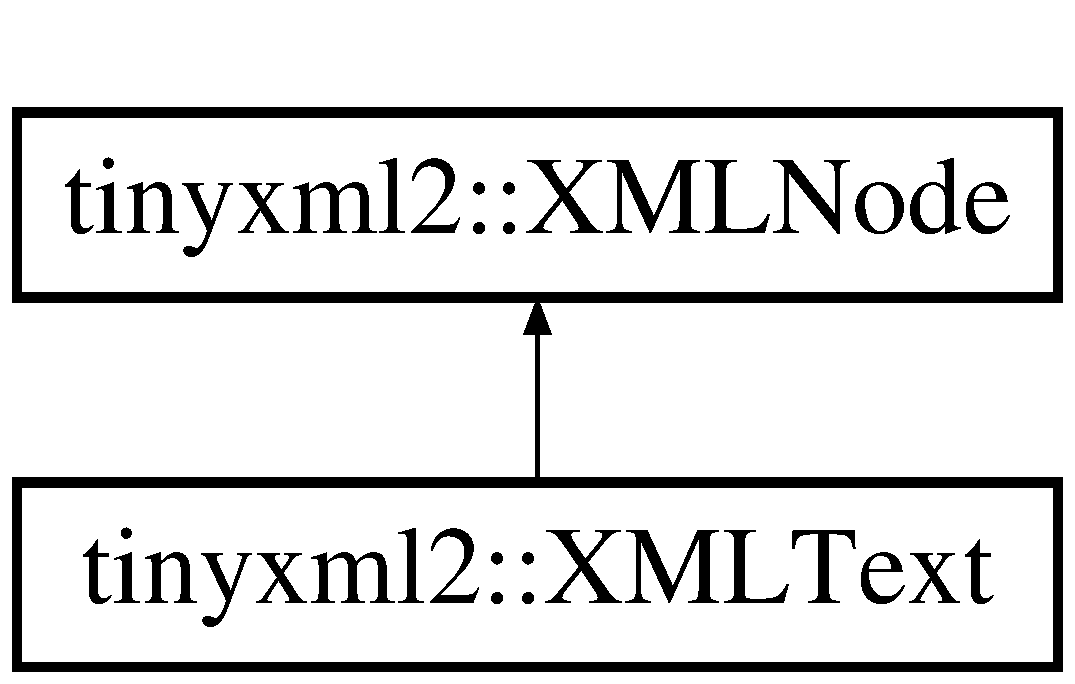
\includegraphics[height=2.000000cm]{classtinyxml2_1_1_x_m_l_text}
\end{center}
\end{figure}
\subsection*{Public Member Functions}
\begin{DoxyCompactItemize}
\item 
virtual bool \hyperlink{classtinyxml2_1_1_x_m_l_text_ae659d4fc7351a7df11c111cbe1ade46f}{Accept} (\hyperlink{classtinyxml2_1_1_x_m_l_visitor}{X\-M\-L\-Visitor} $\ast$visitor) const 
\item 
\hypertarget{classtinyxml2_1_1_x_m_l_text_ab1213b4ddebe9b17ec7e7040e9f1caf7}{virtual \hyperlink{classtinyxml2_1_1_x_m_l_text}{X\-M\-L\-Text} $\ast$ \hyperlink{classtinyxml2_1_1_x_m_l_text_ab1213b4ddebe9b17ec7e7040e9f1caf7}{To\-Text} ()}\label{classtinyxml2_1_1_x_m_l_text_ab1213b4ddebe9b17ec7e7040e9f1caf7}

\begin{DoxyCompactList}\small\item\em Safely cast to Text, or null. \end{DoxyCompactList}\item 
\hypertarget{classtinyxml2_1_1_x_m_l_text_a1e53cbc60968fe966790a65eaf87baaa}{virtual const \hyperlink{classtinyxml2_1_1_x_m_l_text}{X\-M\-L\-Text} $\ast$ {\bfseries To\-Text} () const }\label{classtinyxml2_1_1_x_m_l_text_a1e53cbc60968fe966790a65eaf87baaa}

\item 
\hypertarget{classtinyxml2_1_1_x_m_l_text_ad080357d76ab7cc59d7651249949329d}{void \hyperlink{classtinyxml2_1_1_x_m_l_text_ad080357d76ab7cc59d7651249949329d}{Set\-C\-Data} (bool is\-C\-Data)}\label{classtinyxml2_1_1_x_m_l_text_ad080357d76ab7cc59d7651249949329d}

\begin{DoxyCompactList}\small\item\em Declare whether this should be C\-D\-A\-T\-A or standard text. \end{DoxyCompactList}\item 
\hypertarget{classtinyxml2_1_1_x_m_l_text_a125574fe49da80efbae1349f20d02d41}{bool \hyperlink{classtinyxml2_1_1_x_m_l_text_a125574fe49da80efbae1349f20d02d41}{C\-Data} () const }\label{classtinyxml2_1_1_x_m_l_text_a125574fe49da80efbae1349f20d02d41}

\begin{DoxyCompactList}\small\item\em Returns true if this is a C\-D\-A\-T\-A text element. \end{DoxyCompactList}\item 
\hypertarget{classtinyxml2_1_1_x_m_l_text_ac18d9eec9f12b827b0d02b0847bf279e}{char $\ast$ {\bfseries Parse\-Deep} (char $\ast$, \hyperlink{classtinyxml2_1_1_str_pair}{Str\-Pair} $\ast$end\-Tag)}\label{classtinyxml2_1_1_x_m_l_text_ac18d9eec9f12b827b0d02b0847bf279e}

\item 
virtual \hyperlink{classtinyxml2_1_1_x_m_l_node}{X\-M\-L\-Node} $\ast$ \hyperlink{classtinyxml2_1_1_x_m_l_text_af5115f8cc83de2947ed6a9d13e2f88c8}{Shallow\-Clone} (\hyperlink{classtinyxml2_1_1_x_m_l_document}{X\-M\-L\-Document} $\ast$document) const 
\item 
virtual bool \hyperlink{classtinyxml2_1_1_x_m_l_text_a1588aa5d23cb21eb31f36df0aaaa8d66}{Shallow\-Equal} (const \hyperlink{classtinyxml2_1_1_x_m_l_node}{X\-M\-L\-Node} $\ast$compare) const 
\end{DoxyCompactItemize}
\subsection*{Protected Member Functions}
\begin{DoxyCompactItemize}
\item 
\hypertarget{classtinyxml2_1_1_x_m_l_text_ad9f46d70e61e5386ead93728d8b90267}{{\bfseries X\-M\-L\-Text} (\hyperlink{classtinyxml2_1_1_x_m_l_document}{X\-M\-L\-Document} $\ast$doc)}\label{classtinyxml2_1_1_x_m_l_text_ad9f46d70e61e5386ead93728d8b90267}

\item 
\hypertarget{classtinyxml2_1_1_x_m_l_text_a002156e1f61ee6d48e5368b7cca25582}{{\bfseries X\-M\-L\-Text} (const \hyperlink{classtinyxml2_1_1_x_m_l_text}{X\-M\-L\-Text} \&)}\label{classtinyxml2_1_1_x_m_l_text_a002156e1f61ee6d48e5368b7cca25582}

\item 
\hypertarget{classtinyxml2_1_1_x_m_l_text_ad8c9f398d92fa472e213b89d8483ae8f}{\hyperlink{classtinyxml2_1_1_x_m_l_text}{X\-M\-L\-Text} \& {\bfseries operator=} (const \hyperlink{classtinyxml2_1_1_x_m_l_text}{X\-M\-L\-Text} \&)}\label{classtinyxml2_1_1_x_m_l_text_ad8c9f398d92fa472e213b89d8483ae8f}

\end{DoxyCompactItemize}
\subsection*{Friends}
\begin{DoxyCompactItemize}
\item 
\hypertarget{classtinyxml2_1_1_x_m_l_text_a449202cfc89e7ae5c2f81995476f9ec1}{class {\bfseries X\-M\-L\-Base}}\label{classtinyxml2_1_1_x_m_l_text_a449202cfc89e7ae5c2f81995476f9ec1}

\item 
\hypertarget{classtinyxml2_1_1_x_m_l_text_a4eee3bda60c60a30e4e8cd4ea91c4c6e}{class {\bfseries X\-M\-L\-Document}}\label{classtinyxml2_1_1_x_m_l_text_a4eee3bda60c60a30e4e8cd4ea91c4c6e}

\end{DoxyCompactItemize}
\subsection*{Additional Inherited Members}


\subsection{Detailed Description}
X\-M\-L text.

Note that a text node can have child element nodes, for example\-: \begin{DoxyVerb}<root>This is <b>bold</b></root>
\end{DoxyVerb}


A text node can have 2 ways to output the next. \char`\"{}normal\char`\"{} output and C\-D\-A\-T\-A. It will default to the mode it was parsed from the X\-M\-L file and you generally want to leave it alone, but you can change the output mode with \hyperlink{classtinyxml2_1_1_x_m_l_text_ad080357d76ab7cc59d7651249949329d}{Set\-C\-Data()} and query it with \hyperlink{classtinyxml2_1_1_x_m_l_text_a125574fe49da80efbae1349f20d02d41}{C\-Data()}. 

\subsection{Member Function Documentation}
\hypertarget{classtinyxml2_1_1_x_m_l_text_ae659d4fc7351a7df11c111cbe1ade46f}{\index{tinyxml2\-::\-X\-M\-L\-Text@{tinyxml2\-::\-X\-M\-L\-Text}!Accept@{Accept}}
\index{Accept@{Accept}!tinyxml2::XMLText@{tinyxml2\-::\-X\-M\-L\-Text}}
\subsubsection[{Accept}]{\setlength{\rightskip}{0pt plus 5cm}bool tinyxml2\-::\-X\-M\-L\-Text\-::\-Accept (
\begin{DoxyParamCaption}
\item[{{\bf X\-M\-L\-Visitor} $\ast$}]{visitor}
\end{DoxyParamCaption}
) const\hspace{0.3cm}{\ttfamily [virtual]}}}\label{classtinyxml2_1_1_x_m_l_text_ae659d4fc7351a7df11c111cbe1ade46f}
Accept a hierarchical visit of the nodes in the Tiny\-X\-M\-L-\/2 D\-O\-M. Every node in the X\-M\-L tree will be conditionally visited and the host will be called back via the \hyperlink{classtinyxml2_1_1_x_m_l_visitor}{X\-M\-L\-Visitor} interface.

This is essentially a S\-A\-X interface for Tiny\-X\-M\-L-\/2. (Note however it doesn't re-\/parse the X\-M\-L for the callbacks, so the performance of Tiny\-X\-M\-L-\/2 is unchanged by using this interface versus any other.)

The interface has been based on ideas from\-:


\begin{DoxyItemize}
\item \href{http://www.saxproject.org/}{\tt http\-://www.\-saxproject.\-org/}
\item \href{http://c2.com/cgi/wiki?HierarchicalVisitorPattern}{\tt http\-://c2.\-com/cgi/wiki?\-Hierarchical\-Visitor\-Pattern}
\end{DoxyItemize}

Which are both good references for \char`\"{}visiting\char`\"{}.

An example of using \hyperlink{classtinyxml2_1_1_x_m_l_text_ae659d4fc7351a7df11c111cbe1ade46f}{Accept()}\-: \begin{DoxyVerb}XMLPrinter printer;
tinyxmlDoc.Accept( &printer );
const char* xmlcstr = printer.CStr();
\end{DoxyVerb}
 

Implements \hyperlink{classtinyxml2_1_1_x_m_l_node_a81e66df0a44c67a7af17f3b77a152785}{tinyxml2\-::\-X\-M\-L\-Node}.

\hypertarget{classtinyxml2_1_1_x_m_l_text_af5115f8cc83de2947ed6a9d13e2f88c8}{\index{tinyxml2\-::\-X\-M\-L\-Text@{tinyxml2\-::\-X\-M\-L\-Text}!Shallow\-Clone@{Shallow\-Clone}}
\index{Shallow\-Clone@{Shallow\-Clone}!tinyxml2::XMLText@{tinyxml2\-::\-X\-M\-L\-Text}}
\subsubsection[{Shallow\-Clone}]{\setlength{\rightskip}{0pt plus 5cm}{\bf X\-M\-L\-Node} $\ast$ tinyxml2\-::\-X\-M\-L\-Text\-::\-Shallow\-Clone (
\begin{DoxyParamCaption}
\item[{{\bf X\-M\-L\-Document} $\ast$}]{document}
\end{DoxyParamCaption}
) const\hspace{0.3cm}{\ttfamily [virtual]}}}\label{classtinyxml2_1_1_x_m_l_text_af5115f8cc83de2947ed6a9d13e2f88c8}
Make a copy of this node, but not its children. You may pass in a Document pointer that will be the owner of the new Node. If the 'document' is null, then the node returned will be allocated from the current Document. (this-\/$>$\hyperlink{classtinyxml2_1_1_x_m_l_node_af343d1ef0b45c0020e62d784d7e67a68}{Get\-Document()})

Note\-: if called on a \hyperlink{classtinyxml2_1_1_x_m_l_document}{X\-M\-L\-Document}, this will return null. 

Implements \hyperlink{classtinyxml2_1_1_x_m_l_node_a8402cbd3129d20e9e6024bbcc0531283}{tinyxml2\-::\-X\-M\-L\-Node}.

\hypertarget{classtinyxml2_1_1_x_m_l_text_a1588aa5d23cb21eb31f36df0aaaa8d66}{\index{tinyxml2\-::\-X\-M\-L\-Text@{tinyxml2\-::\-X\-M\-L\-Text}!Shallow\-Equal@{Shallow\-Equal}}
\index{Shallow\-Equal@{Shallow\-Equal}!tinyxml2::XMLText@{tinyxml2\-::\-X\-M\-L\-Text}}
\subsubsection[{Shallow\-Equal}]{\setlength{\rightskip}{0pt plus 5cm}bool tinyxml2\-::\-X\-M\-L\-Text\-::\-Shallow\-Equal (
\begin{DoxyParamCaption}
\item[{const {\bf X\-M\-L\-Node} $\ast$}]{compare}
\end{DoxyParamCaption}
) const\hspace{0.3cm}{\ttfamily [virtual]}}}\label{classtinyxml2_1_1_x_m_l_text_a1588aa5d23cb21eb31f36df0aaaa8d66}
Test if 2 nodes are the same, but don't test children. The 2 nodes do not need to be in the same Document.

Note\-: if called on a \hyperlink{classtinyxml2_1_1_x_m_l_document}{X\-M\-L\-Document}, this will return false. 

Implements \hyperlink{classtinyxml2_1_1_x_m_l_node_a7ce18b751c3ea09eac292dca264f9226}{tinyxml2\-::\-X\-M\-L\-Node}.



The documentation for this class was generated from the following files\-:\begin{DoxyCompactItemize}
\item 
tinyxml2.\-h\item 
tinyxml2.\-cpp\end{DoxyCompactItemize}

\hypertarget{classtinyxml2_1_1_x_m_l_unknown}{\section{tinyxml2\-:\-:X\-M\-L\-Unknown Class Reference}
\label{classtinyxml2_1_1_x_m_l_unknown}\index{tinyxml2\-::\-X\-M\-L\-Unknown@{tinyxml2\-::\-X\-M\-L\-Unknown}}
}


{\ttfamily \#include $<$tinyxml2.\-h$>$}

Inheritance diagram for tinyxml2\-:\-:X\-M\-L\-Unknown\-:\begin{figure}[H]
\begin{center}
\leavevmode
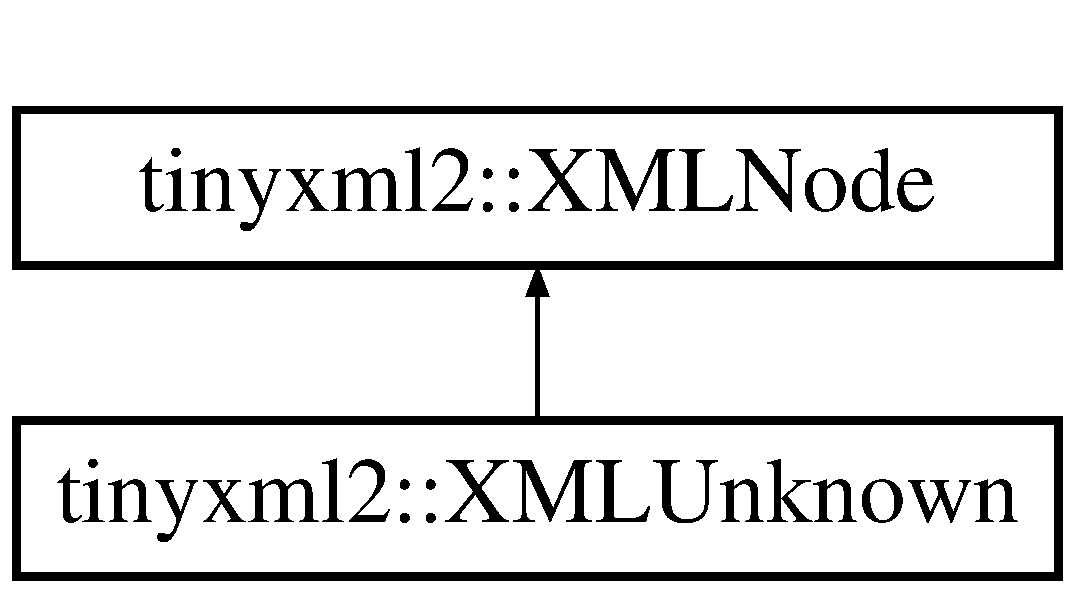
\includegraphics[height=2.000000cm]{classtinyxml2_1_1_x_m_l_unknown}
\end{center}
\end{figure}
\subsection*{Public Member Functions}
\begin{DoxyCompactItemize}
\item 
\hypertarget{classtinyxml2_1_1_x_m_l_unknown_af4374856421921cad578c8affae872b6}{virtual \hyperlink{classtinyxml2_1_1_x_m_l_unknown}{X\-M\-L\-Unknown} $\ast$ \hyperlink{classtinyxml2_1_1_x_m_l_unknown_af4374856421921cad578c8affae872b6}{To\-Unknown} ()}\label{classtinyxml2_1_1_x_m_l_unknown_af4374856421921cad578c8affae872b6}

\begin{DoxyCompactList}\small\item\em Safely cast to an Unknown, or null. \end{DoxyCompactList}\item 
\hypertarget{classtinyxml2_1_1_x_m_l_unknown_a257987e79955399e6e9f119b58d4bb30}{virtual const \hyperlink{classtinyxml2_1_1_x_m_l_unknown}{X\-M\-L\-Unknown} $\ast$ {\bfseries To\-Unknown} () const }\label{classtinyxml2_1_1_x_m_l_unknown_a257987e79955399e6e9f119b58d4bb30}

\item 
virtual bool \hyperlink{classtinyxml2_1_1_x_m_l_unknown_a0d341ab804a1438a474810bb5bd29dd5}{Accept} (\hyperlink{classtinyxml2_1_1_x_m_l_visitor}{X\-M\-L\-Visitor} $\ast$visitor) const 
\item 
\hypertarget{classtinyxml2_1_1_x_m_l_unknown_a0e4f3509dee42a4d45a7f0002be568cc}{char $\ast$ {\bfseries Parse\-Deep} (char $\ast$, \hyperlink{classtinyxml2_1_1_str_pair}{Str\-Pair} $\ast$end\-Tag)}\label{classtinyxml2_1_1_x_m_l_unknown_a0e4f3509dee42a4d45a7f0002be568cc}

\item 
virtual \hyperlink{classtinyxml2_1_1_x_m_l_node}{X\-M\-L\-Node} $\ast$ \hyperlink{classtinyxml2_1_1_x_m_l_unknown_aa09fc7cb0cd64d6bb9c5ae00ffc549ec}{Shallow\-Clone} (\hyperlink{classtinyxml2_1_1_x_m_l_document}{X\-M\-L\-Document} $\ast$document) const 
\item 
virtual bool \hyperlink{classtinyxml2_1_1_x_m_l_unknown_a0169df157bf69a092b404ca49621ff1a}{Shallow\-Equal} (const \hyperlink{classtinyxml2_1_1_x_m_l_node}{X\-M\-L\-Node} $\ast$compare) const 
\end{DoxyCompactItemize}
\subsection*{Protected Member Functions}
\begin{DoxyCompactItemize}
\item 
\hypertarget{classtinyxml2_1_1_x_m_l_unknown_a9391eb679598d50baba424e6f1aa367b}{{\bfseries X\-M\-L\-Unknown} (\hyperlink{classtinyxml2_1_1_x_m_l_document}{X\-M\-L\-Document} $\ast$doc)}\label{classtinyxml2_1_1_x_m_l_unknown_a9391eb679598d50baba424e6f1aa367b}

\item 
\hypertarget{classtinyxml2_1_1_x_m_l_unknown_aab31a93c95a7cedc9597cea7caffa73f}{{\bfseries X\-M\-L\-Unknown} (const \hyperlink{classtinyxml2_1_1_x_m_l_unknown}{X\-M\-L\-Unknown} \&)}\label{classtinyxml2_1_1_x_m_l_unknown_aab31a93c95a7cedc9597cea7caffa73f}

\item 
\hypertarget{classtinyxml2_1_1_x_m_l_unknown_a6137d5611db42c35de3d869f66555e5b}{\hyperlink{classtinyxml2_1_1_x_m_l_unknown}{X\-M\-L\-Unknown} \& {\bfseries operator=} (const \hyperlink{classtinyxml2_1_1_x_m_l_unknown}{X\-M\-L\-Unknown} \&)}\label{classtinyxml2_1_1_x_m_l_unknown_a6137d5611db42c35de3d869f66555e5b}

\end{DoxyCompactItemize}
\subsection*{Friends}
\begin{DoxyCompactItemize}
\item 
\hypertarget{classtinyxml2_1_1_x_m_l_unknown_a4eee3bda60c60a30e4e8cd4ea91c4c6e}{class {\bfseries X\-M\-L\-Document}}\label{classtinyxml2_1_1_x_m_l_unknown_a4eee3bda60c60a30e4e8cd4ea91c4c6e}

\end{DoxyCompactItemize}
\subsection*{Additional Inherited Members}


\subsection{Detailed Description}
Any tag that Tiny\-X\-M\-L-\/2 doesn't recognize is saved as an unknown. It is a tag of text, but should not be modified. It will be written back to the X\-M\-L, unchanged, when the file is saved.

D\-T\-D tags get thrown into X\-M\-L\-Unknowns. 

\subsection{Member Function Documentation}
\hypertarget{classtinyxml2_1_1_x_m_l_unknown_a0d341ab804a1438a474810bb5bd29dd5}{\index{tinyxml2\-::\-X\-M\-L\-Unknown@{tinyxml2\-::\-X\-M\-L\-Unknown}!Accept@{Accept}}
\index{Accept@{Accept}!tinyxml2::XMLUnknown@{tinyxml2\-::\-X\-M\-L\-Unknown}}
\subsubsection[{Accept}]{\setlength{\rightskip}{0pt plus 5cm}bool tinyxml2\-::\-X\-M\-L\-Unknown\-::\-Accept (
\begin{DoxyParamCaption}
\item[{{\bf X\-M\-L\-Visitor} $\ast$}]{visitor}
\end{DoxyParamCaption}
) const\hspace{0.3cm}{\ttfamily [virtual]}}}\label{classtinyxml2_1_1_x_m_l_unknown_a0d341ab804a1438a474810bb5bd29dd5}
Accept a hierarchical visit of the nodes in the Tiny\-X\-M\-L-\/2 D\-O\-M. Every node in the X\-M\-L tree will be conditionally visited and the host will be called back via the \hyperlink{classtinyxml2_1_1_x_m_l_visitor}{X\-M\-L\-Visitor} interface.

This is essentially a S\-A\-X interface for Tiny\-X\-M\-L-\/2. (Note however it doesn't re-\/parse the X\-M\-L for the callbacks, so the performance of Tiny\-X\-M\-L-\/2 is unchanged by using this interface versus any other.)

The interface has been based on ideas from\-:


\begin{DoxyItemize}
\item \href{http://www.saxproject.org/}{\tt http\-://www.\-saxproject.\-org/}
\item \href{http://c2.com/cgi/wiki?HierarchicalVisitorPattern}{\tt http\-://c2.\-com/cgi/wiki?\-Hierarchical\-Visitor\-Pattern}
\end{DoxyItemize}

Which are both good references for \char`\"{}visiting\char`\"{}.

An example of using \hyperlink{classtinyxml2_1_1_x_m_l_unknown_a0d341ab804a1438a474810bb5bd29dd5}{Accept()}\-: \begin{DoxyVerb}XMLPrinter printer;
tinyxmlDoc.Accept( &printer );
const char* xmlcstr = printer.CStr();
\end{DoxyVerb}
 

Implements \hyperlink{classtinyxml2_1_1_x_m_l_node_a81e66df0a44c67a7af17f3b77a152785}{tinyxml2\-::\-X\-M\-L\-Node}.

\hypertarget{classtinyxml2_1_1_x_m_l_unknown_aa09fc7cb0cd64d6bb9c5ae00ffc549ec}{\index{tinyxml2\-::\-X\-M\-L\-Unknown@{tinyxml2\-::\-X\-M\-L\-Unknown}!Shallow\-Clone@{Shallow\-Clone}}
\index{Shallow\-Clone@{Shallow\-Clone}!tinyxml2::XMLUnknown@{tinyxml2\-::\-X\-M\-L\-Unknown}}
\subsubsection[{Shallow\-Clone}]{\setlength{\rightskip}{0pt plus 5cm}{\bf X\-M\-L\-Node} $\ast$ tinyxml2\-::\-X\-M\-L\-Unknown\-::\-Shallow\-Clone (
\begin{DoxyParamCaption}
\item[{{\bf X\-M\-L\-Document} $\ast$}]{document}
\end{DoxyParamCaption}
) const\hspace{0.3cm}{\ttfamily [virtual]}}}\label{classtinyxml2_1_1_x_m_l_unknown_aa09fc7cb0cd64d6bb9c5ae00ffc549ec}
Make a copy of this node, but not its children. You may pass in a Document pointer that will be the owner of the new Node. If the 'document' is null, then the node returned will be allocated from the current Document. (this-\/$>$\hyperlink{classtinyxml2_1_1_x_m_l_node_af343d1ef0b45c0020e62d784d7e67a68}{Get\-Document()})

Note\-: if called on a \hyperlink{classtinyxml2_1_1_x_m_l_document}{X\-M\-L\-Document}, this will return null. 

Implements \hyperlink{classtinyxml2_1_1_x_m_l_node_a8402cbd3129d20e9e6024bbcc0531283}{tinyxml2\-::\-X\-M\-L\-Node}.

\hypertarget{classtinyxml2_1_1_x_m_l_unknown_a0169df157bf69a092b404ca49621ff1a}{\index{tinyxml2\-::\-X\-M\-L\-Unknown@{tinyxml2\-::\-X\-M\-L\-Unknown}!Shallow\-Equal@{Shallow\-Equal}}
\index{Shallow\-Equal@{Shallow\-Equal}!tinyxml2::XMLUnknown@{tinyxml2\-::\-X\-M\-L\-Unknown}}
\subsubsection[{Shallow\-Equal}]{\setlength{\rightskip}{0pt plus 5cm}bool tinyxml2\-::\-X\-M\-L\-Unknown\-::\-Shallow\-Equal (
\begin{DoxyParamCaption}
\item[{const {\bf X\-M\-L\-Node} $\ast$}]{compare}
\end{DoxyParamCaption}
) const\hspace{0.3cm}{\ttfamily [virtual]}}}\label{classtinyxml2_1_1_x_m_l_unknown_a0169df157bf69a092b404ca49621ff1a}
Test if 2 nodes are the same, but don't test children. The 2 nodes do not need to be in the same Document.

Note\-: if called on a \hyperlink{classtinyxml2_1_1_x_m_l_document}{X\-M\-L\-Document}, this will return false. 

Implements \hyperlink{classtinyxml2_1_1_x_m_l_node_a7ce18b751c3ea09eac292dca264f9226}{tinyxml2\-::\-X\-M\-L\-Node}.



The documentation for this class was generated from the following files\-:\begin{DoxyCompactItemize}
\item 
tinyxml2.\-h\item 
tinyxml2.\-cpp\end{DoxyCompactItemize}

\hypertarget{classtinyxml2_1_1_x_m_l_util}{\section{tinyxml2\-:\-:X\-M\-L\-Util Class Reference}
\label{classtinyxml2_1_1_x_m_l_util}\index{tinyxml2\-::\-X\-M\-L\-Util@{tinyxml2\-::\-X\-M\-L\-Util}}
}
\subsection*{Static Public Member Functions}
\begin{DoxyCompactItemize}
\item 
\hypertarget{classtinyxml2_1_1_x_m_l_util_a9333d20f2a34325b5115ca45849c4b2a}{static const char $\ast$ {\bfseries Skip\-White\-Space} (const char $\ast$p)}\label{classtinyxml2_1_1_x_m_l_util_a9333d20f2a34325b5115ca45849c4b2a}

\item 
\hypertarget{classtinyxml2_1_1_x_m_l_util_aa48025be8843ec5a79b65579d31bd8fc}{static char $\ast$ {\bfseries Skip\-White\-Space} (char $\ast$p)}\label{classtinyxml2_1_1_x_m_l_util_aa48025be8843ec5a79b65579d31bd8fc}

\item 
\hypertarget{classtinyxml2_1_1_x_m_l_util_a357ec3af8fc433d19023a815f45e8e33}{static bool {\bfseries Is\-White\-Space} (char p)}\label{classtinyxml2_1_1_x_m_l_util_a357ec3af8fc433d19023a815f45e8e33}

\item 
\hypertarget{classtinyxml2_1_1_x_m_l_util_abe106a69ac4d942a4381a4d9dfd0e0bd}{static bool {\bfseries Is\-Name\-Start\-Char} (unsigned char ch)}\label{classtinyxml2_1_1_x_m_l_util_abe106a69ac4d942a4381a4d9dfd0e0bd}

\item 
\hypertarget{classtinyxml2_1_1_x_m_l_util_a04b17341538fa11752f24b4301d19485}{static bool {\bfseries Is\-Name\-Char} (unsigned char ch)}\label{classtinyxml2_1_1_x_m_l_util_a04b17341538fa11752f24b4301d19485}

\item 
\hypertarget{classtinyxml2_1_1_x_m_l_util_acfcd287cacfd2533e1bc9ea4dfb56602}{static bool {\bfseries String\-Equal} (const char $\ast$p, const char $\ast$q, int n\-Char=I\-N\-T\-\_\-\-M\-A\-X)}\label{classtinyxml2_1_1_x_m_l_util_acfcd287cacfd2533e1bc9ea4dfb56602}

\item 
\hypertarget{classtinyxml2_1_1_x_m_l_util_a24ba87b1d22528167a3d16c4f52096bf}{static int {\bfseries Is\-U\-T\-F8\-Continuation} (const char p)}\label{classtinyxml2_1_1_x_m_l_util_a24ba87b1d22528167a3d16c4f52096bf}

\item 
\hypertarget{classtinyxml2_1_1_x_m_l_util_ae9bcb2bc3cd6475fdc644c8c17790555}{static const char $\ast$ {\bfseries Read\-B\-O\-M} (const char $\ast$p, bool $\ast$has\-B\-O\-M)}\label{classtinyxml2_1_1_x_m_l_util_ae9bcb2bc3cd6475fdc644c8c17790555}

\item 
\hypertarget{classtinyxml2_1_1_x_m_l_util_a5a96e5144a8d693dc4bcd783d9964648}{static const char $\ast$ {\bfseries Get\-Character\-Ref} (const char $\ast$p, char $\ast$value, int $\ast$length)}\label{classtinyxml2_1_1_x_m_l_util_a5a96e5144a8d693dc4bcd783d9964648}

\item 
\hypertarget{classtinyxml2_1_1_x_m_l_util_a31c00d5c5dfb38382de1dfcaf4be3595}{static void {\bfseries Convert\-U\-T\-F32\-To\-U\-T\-F8} (unsigned long input, char $\ast$output, int $\ast$length)}\label{classtinyxml2_1_1_x_m_l_util_a31c00d5c5dfb38382de1dfcaf4be3595}

\item 
\hypertarget{classtinyxml2_1_1_x_m_l_util_a3cd6c703d49b9d51bdf0f4ff6aa021c7}{static void {\bfseries To\-Str} (int v, char $\ast$buffer, int buffer\-Size)}\label{classtinyxml2_1_1_x_m_l_util_a3cd6c703d49b9d51bdf0f4ff6aa021c7}

\item 
\hypertarget{classtinyxml2_1_1_x_m_l_util_ac00c2e52c1c36dab3ff41d86a9bf60f9}{static void {\bfseries To\-Str} (unsigned v, char $\ast$buffer, int buffer\-Size)}\label{classtinyxml2_1_1_x_m_l_util_ac00c2e52c1c36dab3ff41d86a9bf60f9}

\item 
\hypertarget{classtinyxml2_1_1_x_m_l_util_adba0718527ae9e80f663a71ea325cb11}{static void {\bfseries To\-Str} (bool v, char $\ast$buffer, int buffer\-Size)}\label{classtinyxml2_1_1_x_m_l_util_adba0718527ae9e80f663a71ea325cb11}

\item 
\hypertarget{classtinyxml2_1_1_x_m_l_util_a8957ad44fee5fa02ba52d73aad4d0a31}{static void {\bfseries To\-Str} (float v, char $\ast$buffer, int buffer\-Size)}\label{classtinyxml2_1_1_x_m_l_util_a8957ad44fee5fa02ba52d73aad4d0a31}

\item 
\hypertarget{classtinyxml2_1_1_x_m_l_util_a1cd141e50980fcddd6bf9af5de4b1db7}{static void {\bfseries To\-Str} (double v, char $\ast$buffer, int buffer\-Size)}\label{classtinyxml2_1_1_x_m_l_util_a1cd141e50980fcddd6bf9af5de4b1db7}

\item 
\hypertarget{classtinyxml2_1_1_x_m_l_util_ad4df4023d11ee3fca9689c49b9707323}{static bool {\bfseries To\-Int} (const char $\ast$str, int $\ast$value)}\label{classtinyxml2_1_1_x_m_l_util_ad4df4023d11ee3fca9689c49b9707323}

\item 
\hypertarget{classtinyxml2_1_1_x_m_l_util_a210c8637d5eb4ce3d4625294af0efc2f}{static bool {\bfseries To\-Unsigned} (const char $\ast$str, unsigned $\ast$value)}\label{classtinyxml2_1_1_x_m_l_util_a210c8637d5eb4ce3d4625294af0efc2f}

\item 
\hypertarget{classtinyxml2_1_1_x_m_l_util_ae5b03e0a1ca5d42052a7ac540f7aa12a}{static bool {\bfseries To\-Bool} (const char $\ast$str, bool $\ast$value)}\label{classtinyxml2_1_1_x_m_l_util_ae5b03e0a1ca5d42052a7ac540f7aa12a}

\item 
\hypertarget{classtinyxml2_1_1_x_m_l_util_a399e71edb5f29d61ea81d91ee0332bb9}{static bool {\bfseries To\-Float} (const char $\ast$str, float $\ast$value)}\label{classtinyxml2_1_1_x_m_l_util_a399e71edb5f29d61ea81d91ee0332bb9}

\item 
\hypertarget{classtinyxml2_1_1_x_m_l_util_ad8f75ac140fb19c1c6e164a957c4cd53}{static bool {\bfseries To\-Double} (const char $\ast$str, double $\ast$value)}\label{classtinyxml2_1_1_x_m_l_util_ad8f75ac140fb19c1c6e164a957c4cd53}

\end{DoxyCompactItemize}


The documentation for this class was generated from the following files\-:\begin{DoxyCompactItemize}
\item 
tinyxml2.\-h\item 
tinyxml2.\-cpp\end{DoxyCompactItemize}

\hypertarget{classtinyxml2_1_1_x_m_l_visitor}{\section{tinyxml2\-:\-:X\-M\-L\-Visitor Class Reference}
\label{classtinyxml2_1_1_x_m_l_visitor}\index{tinyxml2\-::\-X\-M\-L\-Visitor@{tinyxml2\-::\-X\-M\-L\-Visitor}}
}


{\ttfamily \#include $<$tinyxml2.\-h$>$}

Inheritance diagram for tinyxml2\-:\-:X\-M\-L\-Visitor\-:\begin{figure}[H]
\begin{center}
\leavevmode
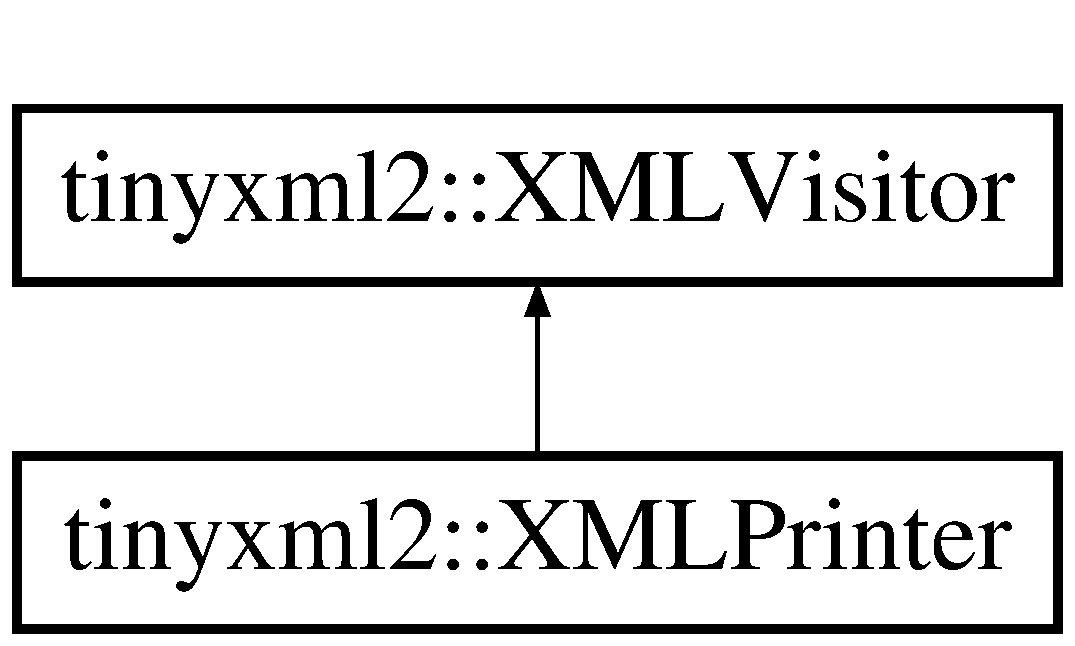
\includegraphics[height=2.000000cm]{classtinyxml2_1_1_x_m_l_visitor}
\end{center}
\end{figure}
\subsection*{Public Member Functions}
\begin{DoxyCompactItemize}
\item 
\hypertarget{classtinyxml2_1_1_x_m_l_visitor_acb3c22fc5f60eb9db98f533f2761f67d}{virtual bool \hyperlink{classtinyxml2_1_1_x_m_l_visitor_acb3c22fc5f60eb9db98f533f2761f67d}{Visit\-Enter} (const \hyperlink{classtinyxml2_1_1_x_m_l_document}{X\-M\-L\-Document} \&)}\label{classtinyxml2_1_1_x_m_l_visitor_acb3c22fc5f60eb9db98f533f2761f67d}

\begin{DoxyCompactList}\small\item\em Visit a document. \end{DoxyCompactList}\item 
\hypertarget{classtinyxml2_1_1_x_m_l_visitor_a170e9989cd046ba904f302d087e07086}{virtual bool \hyperlink{classtinyxml2_1_1_x_m_l_visitor_a170e9989cd046ba904f302d087e07086}{Visit\-Exit} (const \hyperlink{classtinyxml2_1_1_x_m_l_document}{X\-M\-L\-Document} \&)}\label{classtinyxml2_1_1_x_m_l_visitor_a170e9989cd046ba904f302d087e07086}

\begin{DoxyCompactList}\small\item\em Visit a document. \end{DoxyCompactList}\item 
\hypertarget{classtinyxml2_1_1_x_m_l_visitor_af97980a17dd4e37448b181f5ddfa92b5}{virtual bool \hyperlink{classtinyxml2_1_1_x_m_l_visitor_af97980a17dd4e37448b181f5ddfa92b5}{Visit\-Enter} (const \hyperlink{classtinyxml2_1_1_x_m_l_element}{X\-M\-L\-Element} \&, const \hyperlink{classtinyxml2_1_1_x_m_l_attribute}{X\-M\-L\-Attribute} $\ast$)}\label{classtinyxml2_1_1_x_m_l_visitor_af97980a17dd4e37448b181f5ddfa92b5}

\begin{DoxyCompactList}\small\item\em Visit an element. \end{DoxyCompactList}\item 
\hypertarget{classtinyxml2_1_1_x_m_l_visitor_a772f10ddc83f881956d32628faa16eb6}{virtual bool \hyperlink{classtinyxml2_1_1_x_m_l_visitor_a772f10ddc83f881956d32628faa16eb6}{Visit\-Exit} (const \hyperlink{classtinyxml2_1_1_x_m_l_element}{X\-M\-L\-Element} \&)}\label{classtinyxml2_1_1_x_m_l_visitor_a772f10ddc83f881956d32628faa16eb6}

\begin{DoxyCompactList}\small\item\em Visit an element. \end{DoxyCompactList}\item 
\hypertarget{classtinyxml2_1_1_x_m_l_visitor_adc75bd459fc7ba8223b50f0616767f9a}{virtual bool \hyperlink{classtinyxml2_1_1_x_m_l_visitor_adc75bd459fc7ba8223b50f0616767f9a}{Visit} (const \hyperlink{classtinyxml2_1_1_x_m_l_declaration}{X\-M\-L\-Declaration} \&)}\label{classtinyxml2_1_1_x_m_l_visitor_adc75bd459fc7ba8223b50f0616767f9a}

\begin{DoxyCompactList}\small\item\em Visit a declaration. \end{DoxyCompactList}\item 
\hypertarget{classtinyxml2_1_1_x_m_l_visitor_af30233565856480ea48b6fa0d6dec65b}{virtual bool \hyperlink{classtinyxml2_1_1_x_m_l_visitor_af30233565856480ea48b6fa0d6dec65b}{Visit} (const \hyperlink{classtinyxml2_1_1_x_m_l_text}{X\-M\-L\-Text} \&)}\label{classtinyxml2_1_1_x_m_l_visitor_af30233565856480ea48b6fa0d6dec65b}

\begin{DoxyCompactList}\small\item\em Visit a text node. \end{DoxyCompactList}\item 
\hypertarget{classtinyxml2_1_1_x_m_l_visitor_acc8147fb5a85f6c65721654e427752d7}{virtual bool \hyperlink{classtinyxml2_1_1_x_m_l_visitor_acc8147fb5a85f6c65721654e427752d7}{Visit} (const \hyperlink{classtinyxml2_1_1_x_m_l_comment}{X\-M\-L\-Comment} \&)}\label{classtinyxml2_1_1_x_m_l_visitor_acc8147fb5a85f6c65721654e427752d7}

\begin{DoxyCompactList}\small\item\em Visit a comment node. \end{DoxyCompactList}\item 
\hypertarget{classtinyxml2_1_1_x_m_l_visitor_a14e4748387c34bf53d24e8119bb1f292}{virtual bool \hyperlink{classtinyxml2_1_1_x_m_l_visitor_a14e4748387c34bf53d24e8119bb1f292}{Visit} (const \hyperlink{classtinyxml2_1_1_x_m_l_unknown}{X\-M\-L\-Unknown} \&)}\label{classtinyxml2_1_1_x_m_l_visitor_a14e4748387c34bf53d24e8119bb1f292}

\begin{DoxyCompactList}\small\item\em Visit an unknown node. \end{DoxyCompactList}\end{DoxyCompactItemize}


\subsection{Detailed Description}
Implements the interface to the \char`\"{}\-Visitor pattern\char`\"{} (see the Accept() method.) If you call the Accept() method, it requires being passed a \hyperlink{classtinyxml2_1_1_x_m_l_visitor}{X\-M\-L\-Visitor} class to handle callbacks. For nodes that contain other nodes (Document, Element) you will get called with a Visit\-Enter/\-Visit\-Exit pair. Nodes that are always leafs are simply called with \hyperlink{classtinyxml2_1_1_x_m_l_visitor_adc75bd459fc7ba8223b50f0616767f9a}{Visit()}.

If you return 'true' from a Visit method, recursive parsing will continue. If you return false, {\bfseries no children of this node or its siblings} will be visited.

All flavors of Visit methods have a default implementation that returns 'true' (continue visiting). You need to only override methods that are interesting to you.

Generally Accept() is called on the \hyperlink{classtinyxml2_1_1_x_m_l_document}{X\-M\-L\-Document}, although all nodes support visiting.

You should never change the document from a callback.

\begin{DoxySeeAlso}{See Also}
\hyperlink{classtinyxml2_1_1_x_m_l_node_a81e66df0a44c67a7af17f3b77a152785}{X\-M\-L\-Node\-::\-Accept()} 
\end{DoxySeeAlso}


The documentation for this class was generated from the following file\-:\begin{DoxyCompactItemize}
\item 
tinyxml2.\-h\end{DoxyCompactItemize}

%--- End generated contents ---

% Index
\newpage
\phantomsection
\addcontentsline{toc}{part}{Index}
\printindex

\end{document}
